\documentclass[MScCS]{uccthesis}
%\title{The \texttt{uccthesis} Class}
\title{Allergy Management with Mobile App - AllerTeens}
\author{Vedant Vijay Salvekar}
\supervisor{Dr. Dirk Pesch}
\secondreader{Dr. Andrea Visentin}
\date{\today}
\usepackage{biblatex} %Imports biblatex package
\usepackage[hidelinks]{hyperref}
\usepackage{tabularx} % put in preamble

\newcommand*{\COMMAND}[1]{\texttt{\textbackslash #1}}
\newcommand*{\COMMANDWITHARGUMENT}[2]{\texttt{\textbackslash #1}\{#2\}}

\addbibresource{mybib.bib}% should be in preamble




\abstract{%

Severe food allergies, such as peanut allergies, pose numerous difficulties for adolescents as they age and shift from parent support to independent self-management. These difficulties go beyond the medical dangers of accidental contact and anaphylactic reaction to social concerns like anxiety, disclosure to peers, and social navigation. Although there are some educational materials on allergies, there is a lack of interactive and context-specific resources that adolescents can use to practice realistic allergy self-management. \textit{AllerTeens} is a cross-platform mobile health application developed in collaboration with UCC School of Nursing and Midwifery and Cork University Hospital's Paediatric Allergy Unit. The app was built in Flutter and incorporates practical features including barcode scanning, reminders for adrenaline pens, logs for accidental exposures, and a "Learn" module which integrates relevant clinical, behavioural, and psychosocial information. The app's major innovation lies in scenario-driven AI training with Large Language Models like OpenAI's GPT-3.5-turbo, allowing adolescents to role-play safe conversations in restaurants, parties, and peer gatherings and receive adaptive feedback to reinforce safe behaviours. Evaluation was conducted with six adolescents in three structured group sessions. Task completion was rated 4-5 on ease, usefulness, and enjoyment, with AI scenarios rated as the most engaging. Although there were suggestions for improvement such as providing clearer voice input instructions or reminders tailored for specific events, the overall conclusions support the effectiveness and acceptability of AI-enabled interventions for the self-management of allergies in adolescents.


}


\acknowledgement{%
  I would like to thank my supervisors, Dr.~Dirk Pesch and Dr.~Andrea Visentin, without whose strong guidance, encouragement and support this project would have been incomplete. Their knowledge and productive comments have played a vital role in defining the nature and results of this research. I would also like to express my thanks to Malik Qirtas with whom I had numerous and always valuable discussions which enabled me to keep my head focused and develop at a steady pace.  I am also deeply grateful to Megan O'Sullivan, who worked in parallel on the medical aspects of this research. Her collaboration throughout the process, particularly in facilitating focus group meetings and contributing clinical documentation, was instrumental in bridging the technical and medical dimensions of this work.   We would like to thank the Paediatric Allergy Unit at Cork University Hospital (CUH), without whose clinical expertise and cooperation this work would be less grounded in the real-world health needs. Their feedback played an important role in verifying that their needs were captured by the application and that the medical and the psychosocial issues surrounding individuals with severe food allergies were discussed using this tool. Finally, I would like to extend my heartfelt appreciation to my friends and family.

}

\renewcommand\addToFrontMatter[0]{%
}

\begin{document}

\chapter{Introduction}


% \section{Problem Statement} 
Allergic conditions raise global health issues, especially for minors and adolescents. Research shows that around 8\% of children have food allergies, with nut allergies considered among the most common \cite{sullivan2024telehealth}. For teenagers who are beginning to self-manage, these conditions are particularly challenging because they require strict adherence to self-care guidelines and emergency protocols.  

The University College Cork (UCC) School of Nursing and Midwifery, in collaboration with the Paediatric Allergy Unit at Cork University Hospital, is exploring ways to assist adolescents during this period of transition. One of the most promising telehealth supports for self-care is the use of mHealth applications. Research indicates that mobile apps are the most frequently used digital tools, followed by interventions such as video conferencing, web platforms, VR, and AI \cite{majeed2015apps}. However, there remains insufficient analysis of the long-term efficacy and sustained impact of these technologies.  

Adolescents self-managing their allergies stand to gain the most from accessible digital health interventions. While mobile apps are increasingly applied in chronic condition management, the use of gamification, interactive learning tools, and scenario-based training remains underutilized in allergy care \cite{sullivan2024telehealth, broome2021fasst}.  

Despite advances in telehealth, creating a robust self-management system remains challenging. These challenges include:
\begin{itemize}
    \item Increasing reliance on digital assistance combined with restricted access to allergy specialists.
    \item Lack of structured and validated self-management tools tailored for adolescents.
    \item Low engagement and adherence to existing digital health solutions.
    \item The need to integrate educational, behavioral, psychosocial, and emergency response features into a single platform \cite{kwen2022foodallergy}.
\end{itemize}

The problem becomes all the more important given the hospital admission rates for anaphylaxis, they have more than tripled over the last few decades \cite{matricardi2020mhealth}. Waiting lists for allergy specialists in Ireland highlight the need for self-management solutions that are both digital and more readily available.  

While some digital tools exist, there remains a significant gap in providing adolescents with realistic, scenario-based training for allergy self-management. Current solutions often emphasize static educational resources, but lack interactive practice environments that mirror the challenges teenagers face in social contexts such as restaurants, parties, or peer-group settings. This dissertation seeks to address this gap through the design and development of \textit{AllerTeens}, a mobile application that leverages artificial intelligence to deliver dynamic and context-aware training scenarios.  
 
The app has the ability of using AI-powered voice acknowledgement and simulations, which help teenagers practice allergy disclosure and decision-making under peer pressure, along with emergency preparedness in secure but lifelike conditions. All of these features can be integrated with symptom tracking, accidental exposure logging, adrenaline pen reminders and structured education to provide a comprehensive self management platform. The idea is to make adolescents feel knowledgeable and capable of handling themselves and limiting anxiety levels, gaining independence in the process.

In doing so, \textit{AllerTeens} contributes to closing the gap between conventional educational interventions and practical, interactive self-management tools, laying the foundation for future clinical evaluation and large-scale deployment.  
\clearpage




\section{Project Overview}
\textit{AllerTeens} is a mobile health application that aims to assist adolescents with severe food allergies to make the transition to self-management of their condition. The application is built in collaboration with UCC School of Nursing and Midwifery and Paediatric Allergy Unit at CUH; it combines educational, behaviour and psychosocial supports with interactive and innovative training modules. The system is more than a general allergy education and symptom tracker, as it simulates realistic everyday scenarios, such as ordering food in restaurants, attending social events, or reacting to accidental exposures. Its core interest is to establish confidence, enhance decision making, and equip teenagers to feel safe about self-management in real situations.  

\subsection*{Core Features}
\begin{itemize}
    \item \textbf{AI Training Scenarios:} Interactive, scenario-based conversations powered by speech-to-text and text-to-speech. Includes waiter simulations and group scenarios (e.g., birthday parties, dinners with friends) to practice allergy disclosure and decision-making under peer pressure.
    \item \textbf{Scenario Progression \& Feedback:} Level-based difficulty (Beginner, Intermediate, Advanced) with contextual feedback, safety checks, scoring, and mastery badges to encourage skill development and resilience.
    \item \textbf{Group Conversation Simulation:} Multi-character dialogues with distinct voices and avatars, allowing adolescents to rehearse managing peer interactions in challenging social contexts.
    \item \textbf{Gamified Progress Tracking:} Achievements, mastery indicators, and progress streaks motivate repeated engagement while storing attempts and outcomes in Firestore for long-term monitoring.
    \item \textbf{Barcode Scanning:} Camera-based scanning of packaged foods to check for allergens, with manual entry fallback.
    \item \textbf{Symptom and Exposure Logging:} Calendar-based tracking of accidental exposures, symptom severity, treatment responses, and notes.
    \item \textbf{Adrenaline Pen Reminders:} Customisable notifications prompting users to confirm whether they are carrying their pen, with integrated calendar markers.
    \item \textbf{Educational and Behavioural Content:} Integrated "Learn" module presenting structured information on allergen management, psychosocial coping strategies, and behavioural guidance in an accessible, adolescent-friendly format.
    \item \textbf{Emergency Contact Access:} One-tap access to call a designated emergency contact directly from the home screen.
\end{itemize}

The primary objective of \textit{AllerTeens} is to provide an effective, engaging, and accessible digital tool that empowers adolescents to build self-agency, practice safe behaviours, and gain confidence in allergy self-management. By blending interactive AI-driven training with practical support tools such as symptom logging, reminders, and educational resources, the app aims to address not only the medical but also the psychosocial challenges of living with severe food allergies.  

Effective project management underpinned the development of the application. A structured GitHub repository was maintained to centralise all source code, documentation, and feature tracking, ensuring accountability and version control.   


Chapter 2 discusses the background literature with a review on the problems posed by allergies among adolescents, mobile health (mHealth) interventions, and their current applications, as well as the gaps in the ecosystem. Chapter 3 describes the methodology that incorporates collaboration with clinical stakeholders, PPI sessions, supporting materials, relevant ethics, and the entire development cycle. Chapter 4 focuses on the system design, detailing the architectural overview, technical frameworks, minimum viable product (MVP), and critical design constraints. In Chapter 5, the focus is placed on the implementation of the application with the AI training segment for the daily reminders, symptom logging, barcode scanning, and the use of Firebase services. Chapter 6 discusses the adolescents and clinical experts feedback on the evaluation methodology and the supervisors comments on the evaluation findings. Chapter 7 rounds the thesis discussing the contributions, limitations, and the identified opportunities for growth.



\begin{figure}[htbp]
    \centering
    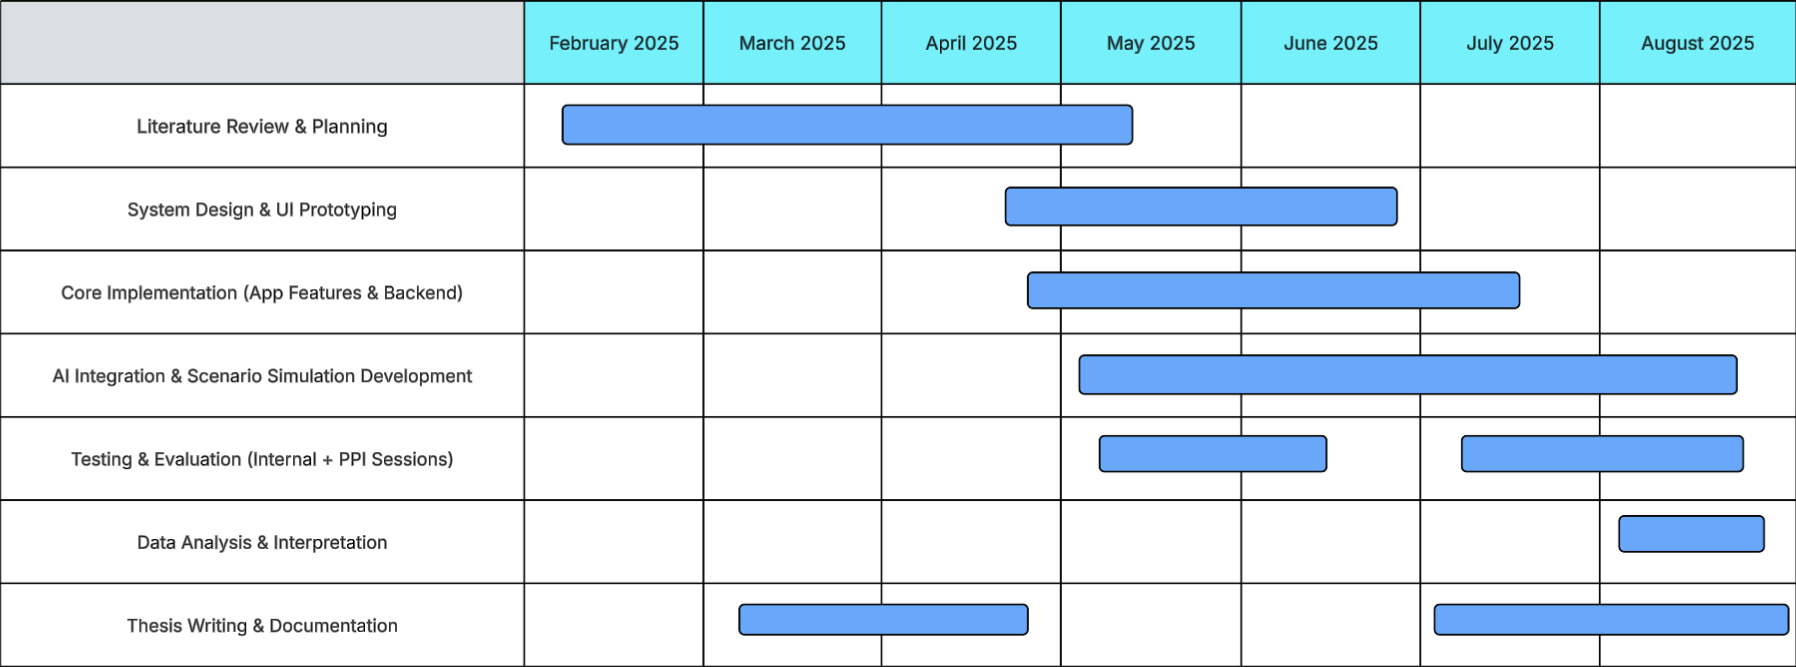
\includegraphics[width=\textwidth]{Figures/gantt_chart.png}
    \caption{High-level project activity Gantt chart showing development phases from February to August 2025}
    \label{fig:gantt}
\end{figure}

\clearpage
 

\chapter{Background and Literature Review}


Adolescents with life-threatening allergies face considerable challenges when transitioning to self-management. Mobile health (mHealth) apps offer a scalable, digital approach for delivering education, symptom tracking, emergency protocols, and personalized care \cite{matricardi2020mhealth, sullivan2024telehealth}. However, as highlighted in several studies, the current ecosystem of allergy-related apps suffers from fragmented features, lack of adolescent-specific engagement, and limited use of advanced techniques such as gamification and interactive simulation \cite{virella2019mobile, majeed2015apps, macmath2023ai, gajardo2023gamification}.  

This chapter explores the core concepts, technologies, and existing applications in allergy management. It analyzes design approaches, identifies gaps, and positions the proposed integrated solution AllerTeens within the existing literature.

\section{Concepts, Technologies, and Fundamentals}

This section gives the theoretical and technological foundations of self-management of allergies among the adolescents. It starts with an overview of the peculiarities of challenges of adolescents, and then proceeds to the importance of mHealth, digital interventions, and the technologies, which make the former two roadable supporting technologies, including gamification and AI. These ideas provide the background on which \textit{AllerTeens} is based on its design and implementation.

\subsection{Overview of Adolescent Allergy Challenges}
From an adolescent's viewpoint, the most common allergic disorders encompass food allergies, asthma, eczema, and allergic rhinitis. This dissertation concentrates on \textbf{food allergies}, which pose specific dangers of anaphylaxis in typical daily situations. It is relevant to mention that most telehealth solutions for adolescents with allergic disorders have been aimed at asthma management. Along with balancing school and friendships, young adolescents require a certain degree of independence. Emotional and behavioral changes in mid and late adolescence often result in erratic inconsistencies in following allergy management routines. As highlighted by Sullivan et al.~\cite{sullivan2024telehealth}, the treatment gap in adolescence stems from a lack of awareness for the condition, underdeveloped executive functioning, considerable social pressure, and overwhelming external social dynamics.



The transition to independence typically occurs between ages 11 and 19, a stage when most adolescents are not fully prepared. Barriers include forgetfulness, fear of social labeling, difficulties navigating healthcare systems, and absence of structured training. Sullivan et al.~\cite{sullivan2024telehealth} identify five major domains of transition support: education, skill acquisition, self-efficacy, peer engagement, and provider support. Without structured interventions, adolescents may either remain overly dependent on caregivers or feel overwhelmed by self-management demands.

\subsection{The Role of mHealth in Allergy Care}
mHealth extends the capability of mobile devices to put appropriate chronic care tools at people. In allergy management, this comprises of symptom tracking, recording medication use, obtaining education resources, and emergency response strategies. According to Matricardi et al.~\cite{matricardi2020mhealth}, mHealth enhances access to care, continuity, and self-efficiency in the management of allergies. Telehealth applications have a possibility to make youth autonomous due to interactive and user-centric content \cite{sullivan2024telehealth}.

\subsection{Importance of Digital Interventions for Teen Users}
Adolescent users require digital interventions that combine education with interactive learning and peer relevance. Mobile apps designed for teenagers are most effective when they provide self-governance, attractive visual design, and flexible learning methods \cite{perez2019mobile}. Sullivan et al.~\cite{sullivan2024telehealth} emphasize that adolescent-focused systems must enhance decision-making capabilities, reduce isolation, and promote engagement through features that mirror real-life contexts.

\subsection{Core Technologies and Supporting Strategies}
\label{sec:core-tech}

Several technological and design strategies are highlighted in the literature as being particularly relevant to adolescent-focused allergy management. These include:

\begin{enumerate}
    \item \textbf{Mobile Health (mHealth) Applications}  
    mHealth apps are widely applied in chronic disease management and increasingly in allergy care. Common features include exposure logging, allergen identification, educational resources, and reminder notifications \cite{matricardi2020mhealth}. Such tools contribute to adherence and safety, but studies indicate that existing allergy apps often lack customization for adolescent users \cite{virella2019mobile}. Research underscores the need for age-appropriate interfaces, simplified workflows, and adaptive content to sustain adolescent engagement \cite{sullivan2024telehealth}.  

    \item \textbf{Gamification Techniques}  
    Health apps often use gamification as an incentive or adherence driver. Engagement has been found to be improved by the use of strategies, including rewards, levels, progress streaks, and mastery badges, especially among younger users \cite{gajardo2023gamification, tran2022gamification}. Examples such as asthma and diabetes apps where medical literacy and self-management skills can be reinforced by gamified learning modules. Nonetheless, there is an underutilization of gamification in allergy-specific digital programs, even though its potential has been demonstrated \cite{broome2021fasst}.

    \item \textbf{Artificial Intelligence (AI) in Health Applications}  
    AI has been explored in allergy care primarily through chatbots, symptom-checking systems, and adaptive e-learning tools \cite{macmath2023ai}. These systems provide scalability and real-time personalization, but they face limitations around clinical accuracy, ethical validation, and contextual adaptation \cite{bajowala2022telehealth}. To date, the literature reports no widespread use of immersive AI-driven simulations for allergy management; instead, most existing AI applications focus on structured Q\&A, risk assessment, and decision-support frameworks \cite{majeed2015apps, sullivan2024telehealth}. This gap indicates potential for novel approaches but also highlights the need for robust evaluation frameworks.  

    \item \textbf{User Interface Design Principles for Adolescents}  
    Adolescent-focused health apps must address developmental, cognitive, and accessibility needs. Research suggests that adolescents prefer clear navigation, visually appealing interfaces, voice-guided content, and modular information delivery \cite{kwen2022foodallergy}. Studies emphasize the role of personalization and visual progress indicators in increasing adherence and satisfaction among teen users \cite{perez2019mobile}.  

    \item \textbf{Offline Capability in Emergency Health Apps}  
    Access to reliable emergency information is critical during allergy incidents, which may occur in areas with limited connectivity. Perez et al.~\cite{perez2019mobile} highlight that offline caching of emergency protocols and decision trees improves usability and safety. Nevertheless, many existing health apps still rely heavily on continuous internet connectivity, limiting their effectiveness in real-world emergencies.  

    \item \textbf{Legal and Ethical Considerations}  
    Adolescent mHealth systems must comply with regulatory frameworks such as GDPR. Literature stresses the importance of anonymization, data encryption, and parental consent in safeguarding young users \cite{bajowala2022telehealth}. Ethical considerations for AI-based health tools include explainability, transparency in decision-making, and mitigation of bias in recommendations \cite{macmath2023ai}. Studies warn that lack of oversight can lead to misinformation and reduced trust among users \cite{sullivan2024telehealth}.  
\end{enumerate}



\section{Review of Existing Allergy and Health Management Apps}
This section analyzes mobile applications focused on food allergies and related chronic conditions. The review outlines progress to date, highlights shortcomings in existing solutions, and positions \textit{AllerTeens} in relation to other applications as a means to showcase its unique value.


\subsection{Market Analysis}

In the landscape of food allergy management, a number of mHealth applications have been developed to provide support for patients and caregivers. While these platforms deliver valuable resources such as symptom logging, emergency protocols, and peer community spaces, they remain limited in adolescent-specific engagement, integration, and adaptive learning.  

\paragraph{Allergy Force}  
Allergy Force positions itself as a comprehensive allergy companion app. It offers emergency protocols, barcode scanning for allergen identification, and reminders for carrying medication. While effective as a functional tool, research highlights that its design is primarily utilitarian and lacks features specifically tailored for adolescents, such as gamified learning or interactive training environments \parencite{matricardi2020mhealth}.  

\paragraph{Spokin}  
Spokin focuses on peer support by crowdsourcing allergy-friendly restaurant and product reviews. It builds a community of allergy-aware families, but it functions largely as a directory and social sharing platform. The app does not include structured training for emergency preparedness or adolescent-specific self-management features \parencite{broome2021fasst}.  

\paragraph{ASTHMAXcel Adventures}  
Although designed for asthma education, ASTHMAXcel demonstrates the potential of gamification in health management. Through avatars, storytelling, and level-based challenges, it engages younger users in interactive learning \parencite{tran2022gamification}. While it does not address food allergies directly, it provides a strong example of how gamification can reinforce medical literacy and self-efficacy in chronic illness care.  

\paragraph{Bearable}  
Bearable is a general health app emphasizing symptom and mood tracking. It helps users identify lifestyle and health correlations but is not designed for allergy-specific needs. Its broad focus reduces its usefulness in critical allergy contexts, such as accidental exposure or emergency readiness.  

\paragraph{}Taken together, these applications highlight the diversity of approaches in allergy and chronic health management. Table~\ref{tab:app-feature-analysis} provides a comparative overview of their core features, with a particular focus on emergency protocols, AI integration, gamification, community support, and adolescent usability.

% \subsection{Comparative Feature Analysis}

\begin{table}[htbp]
\centering
\small
\caption{Feature Comparison of Selected Allergy Management Apps}
\label{tab:app-feature-analysis}
\renewcommand{\arraystretch}{1.3}
\setlength{\tabcolsep}{10pt}
\begin{tabular}{|l|c|c|c|c|c|}
\hline
\textbf{App} & \textbf{Emergency} & \textbf{AI} & \textbf{Gamifi-} & \textbf{Community} & \textbf{Teen} \\
\textbf{Name} & \textbf{Protocols} & \textbf{Support} & \textbf{cation} & \textbf{Support} & \textbf{Usability} \\
\hline
Allergy Force     & Yes & No  & No  & Yes & Low \\
Spokin            & No  & No  & No  & Yes & Medium \\
Bearable          & No  & No  & No  & No  & Medium \\
ASTHMAXcel        & No  & No  & Yes & No  & High \\
\hline
\end{tabular}
\end{table}

\subsection{Gaps in Current Ecosystem for Adolescents}

Despite the growing number of mobile apps in the allergy and chronic health space, several gaps remain:  

\begin{itemize}
    \item \textbf{Lack of Integration:} Existing apps tend to specialize in a single function (e.g., emergency protocols, community reviews, or symptom tracking) rather than offering a holistic solution.  
    \item \textbf{Insufficient Youth Engagement:} Interfaces are often designed for adults or caregivers and do not reflect the motivational or psychosocial needs of teenagers \parencite{sullivan2024telehealth}.  
    \item \textbf{Underuse of Smart Features:} AI-based personalization, interactive simulations, and gamified learning shown to be effective in other health domains remain underutilized in allergy-specific apps \parencite{macmath2023ai, gajardo2023gamification}.  
    \item \textbf{Limited Offline Functionality:} Many apps rely heavily on internet connectivity, despite emergencies often occurring in offline contexts \parencite{perez2019mobile}.  
\end{itemize}
\clearpage

\chapter{Methodology and Requirements Gathering}
\label{chap:methodology}

The development of the AllerTeens application followed a participatory design methodology, integrating both clinical expertise and direct input from adolescents living with severe food allergies. This approach ensured that the resulting features addressed real-world needs rather than being solely researcher-driven.

\section{Collaboration with Clinical Partners}
Preliminary meetings were done with the Paediatric Allergy Unit at the Cork University Hospital (CUH) where the research team got to understand the essential goals of the project and could point out the areas of greatest need of digital intercession. This preliminary discourse initially informed the framework of the application which centered around an adolescent-focused on self-management, emergency preparedness.

\section{Patient and Public Involvement (PPI) Sessions}
\label{sec:ppi-sessions}
To embed adolescent perspectives in the design, Patient and Public Involvement (PPI) sessions were arranged with six teenagers who volunteered to contribute. Eligible participants were adolescents aged 12-16, attending the Cork University Hospital (CUH) Paediatric Allergy service, diagnosed with at least one food allergy and prescribed an Adrenaline Auto-Injector (AAI).The process was structured into three phases:

\subsection*{Session 1 - Introduction and Brainstorming}
The participants were presented with information about the project objectives, and requested to present their everyday difficulties regarding allergy management. Some of the major concerns expressed were failure to carry adrenaline auto-injectors due to forgetfulness, challenges encountered when disclosing allergies in social situations, and fear of eating outside.

\subsection*{Session 2 - Feature Discussion and Refinement}
The next step was a discussion with teens, which was more hands-on, showing some concepts such as the AI training simulation. As the teens gave feedback, they were guided by a loose set of prompt questions which were designed to help their thoughts remain relevant to the project. This mixture of structure and freedom helped achieve the project goals.
 

\begin{table}[htbp]
\centering
\small
\caption{Guiding questions used during Session 2 discussions}
\label{tab:ppi-session2-questions}
\renewcommand{\arraystretch}{1.2}
\begin{tabular}{|c|p{10cm}|}
\hline
\textbf{No.} & \textbf{Question} \\
\hline
1 & What are your thoughts on the educational content provided by CUH? \\
2 & What are your thoughts on the behavioural content? \\
3 & Do you have any ideas for features you would like to see in the app? \\
4 & Do you have any suggestions for possible app names? \\
\hline
\end{tabular}
\end{table}

Key outcomes from this discussion included:  
\begin{itemize}
    \item A reminder system linked to a calendar, allowing users to confirm whether they carried their adrenaline pen on a given date (logged as "Yes/No").
    \item Scenario-based AI training focused on real-life contexts highlighted by participants, such as restaurants, dinners with friends, parties, and school trips.
    \item Enhancements to accidental exposure logs, including an additional field for "food eaten" to capture contextual details of incidents.
\end{itemize}

A final session was later held to validate the refined features and collect additional ideas for improvements and future enhancements. While feedback from this session contributed to shaping long-term development goals, the outcomes of user evaluation are discussed separately in Chapter~\ref{chap:evaluation}.

\subsection*{Evaluation Method}
During both requirements gathering and later evaluation (Chapter~\ref{chap:evaluation}), adolescents were asked to rate core tasks on a five-point Likert scale to capture usability and engagement. The scale was defined as: 
\begin{itemize}
    \item 1 = Very difficult / not useful / not enjoyable 
    \item 2 = Difficult / limited usefulness / low enjoyment
    \item 3 = Neutral / acceptable but with limitations
    \item 4 = Easy to use / useful / enjoyable 
    \item 5 = Very easy / highly useful / highly enjoyable
\end{itemize}
This structured scoring allowed feedback to be compared systematically across participants while retaining the qualitative insights captured through open discussion.



\section{Supporting Resources and Reference Materials}
To ensure the app design was grounded in evidence-based practice, the study drew on a range of structured resources provided by the Paediatric Allergy Unit at Cork University Hospital (CUH). These included clinical guidelines, patient information leaflets, and documents on educational, behavioural, and psychosocial management of food allergies. The content from these resources informed the \textit{Learn} module of the application, ensuring that information was clinically accurate, age-appropriate, and relevant to adolescent experiences. A full list of source materials is included in Appendix~\ref{app:resources}.  

All content integrated into the application was reviewed and validated by a panel of medical professionals, including a Consultant Paediatric Allergist, a Clinical Nurse Specialist in Paediatric Allergy, a Paediatrician with a Special Interest in Allergy (Northern Ireland), a Dietician with a Special Interest in Allergy, and a Psychologist with a Special Interest in Allergy. Their input ensured that the educational and psychosocial materials reflected best clinical practice and supported holistic adolescent care.  

In addition to textual resources, discussions with clinicians highlighted the need for practical digital tools such as symptom logs, adrenaline pen reminders, and food allergen identification. This feedback directly shaped the inclusion of features such as the barcode scanner, allowing adolescents to check packaged foods against allergen risks in everyday contexts. Together, these resources and validations ensured that the application combined clinical rigour with usability for adolescents.
 

\section{Ethical Considerations}
Working with adolescents and health-related information required adherence to strict ethical and legal standards. Participation in Patient and Public Involvement (PPI) sessions was voluntary, with informed consent obtained from both the adolescents and their parents/guardians. All identifying information was anonymised, and only aggregated feedback was recorded for analysis.  

In line with GDPR and Health Research Regulations (2018/2021), no personal health data were stored or processed during the research phase. Instead, discussions focused on hypothetical scenarios, user needs, and design preferences. The development process also incorporated privacy-by-design principles, ensuring that features such as reminders, symptom logging, and profile storage were designed with secure handling and minimal data exposure.  

Formal ethical approval for this study was granted by the \textit{Clinical Research Ethics Committee of the Cork Teaching Hospitals (CREC)}. Approval was issued on \textbf{4th June 2025}, under CREC Review Reference Numbers \textbf{ECM 4 (v) 15/05/2025} and \textbf{ECM 3 (b) 15/06/2025}.  



\section{Development Process}
The design was based on an iterative user-centered process. Example of early prototypes and proof-of-concept (POC) features (e.g., the AI training simulation) were discussed at PPI sessions, facilitating the feedback process by the adolescents before full implementation. An Agile-like approach was used, with frequent iterating, testing, and gathering feedback and integrating it with the stakeholders. This iterative process ensured the application evolved in alignment with both clinical objectives and adolescent user expectations.

Version control was maintained via GitHub, enabling structured management of source code, documentation, and issue tracking. This ensured accountability and facilitated rapid iteration. Project scheduling and task management were supported by Gantt chart visualisations, which allowed the development process to remain on track and adapt to potential bottlenecks.
\clearpage


\chapter{System Design}

This chapter describes the system of the \textit{AllerTeens}. The design focuses on scaling, accessibility and cortex amounts towards the adolescent-specific engagement without compromising safety and adherence in treating severe food allergies. The next sections present the architecture, the user interface characteristics, and design of the important modules, and design principles that treat issues of the data security, reliability offline and ethical compliance.

\section{System Architecture Overview}
The AllerTeens system is built as a cross-platform mobile application developed in Flutter and Dart, supported by Firebase services for authentication, cloud data storage, and synchronization. The architecture follows a modular design to allow iterative development and integration of new features.

\begin{figure}[htbp]
    \centering
    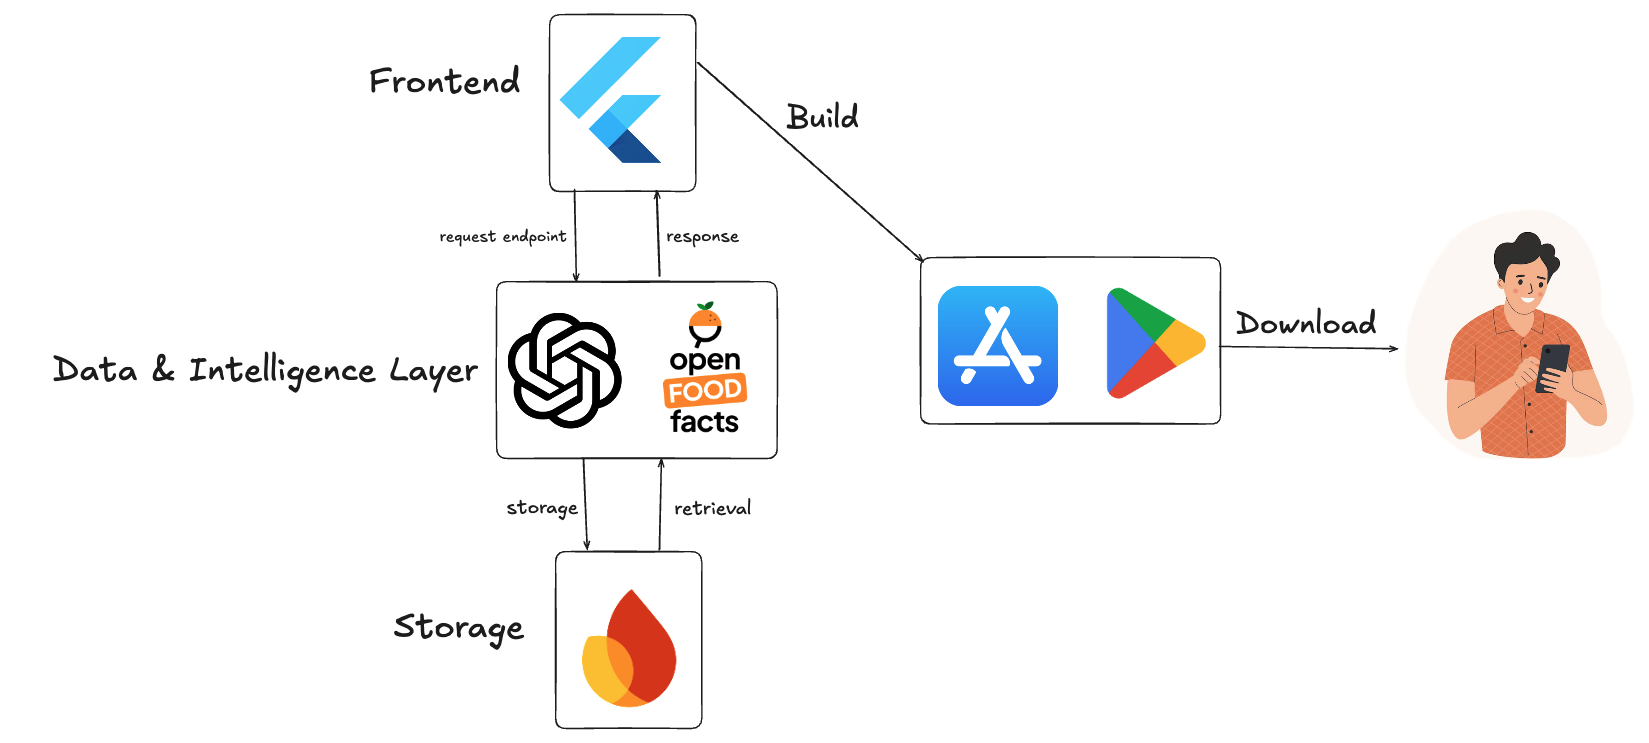
\includegraphics[width=\textwidth]{Figures/high_level_system_architecture.png}
    \caption{High-level System Architecture of AllerTeens}
    \label{fig:system-architecture}
\end{figure}

The high-level architecture (Figure \ref{fig:system-architecture}) shows how the Flutter client communicates with AI services, Firebase storage, and external APIs such as OpenFoodFacts and CUH Docs. At its core, the design separates concerns into three layers: the client-facing Flutter app, the data and intelligence services, and persistent cloud storage.  


The component architecture emphasizes modularity:
\begin{itemize}
    \item \textbf{Flutter Client:} UI, profile setup, training scenarios, logs, reminders, barcode scanning, and offline modules.
    \item \textbf{Firebase Services:} Authentication, Firestore DB for structured logs and progress, Cloud Storage for documents and action plans.
    \item \textbf{AI Simulation Service:} Includes speech-to-text, text-to-speech, scenario engine, and adaptive feedback \& scoring loop.
    \item \textbf{Notification System:} Local notifications for reminders.
    \item \textbf{External Data Sources:} OpenFoodFacts API for barcode lookups and CUH Docs for validated clinical action plans.
\end{itemize}

\section{Technical Frameworks}
The system relies on a set of frameworks chosen to maximize reliability, scalability, and speed of development.  

\subsection{Flutter and Dart}
Flutter was selected because of its cross platform support, which allows running on both iOS and Android with a shared codebase. It has a widget-based architecture that enables the design of a modular interface, as well as rapid prototyping with hot reloading. Dart can be used with Flutter to give it an object oriented, concise syntax that is good at client facing applications that are reactive.

Flutter also makes available a large number of third-party packages (e.g., speech-to-text, barcode scanning, Firebase SDKs), which saved effort and increased system reliability.

In practice, the dependency ecosystem defined in the \texttt{pubspec.yaml} file (Figure~\ref{fig:pubspec}) illustrates the breadth of functionality integrated into the app. Core libraries included \texttt{firebase\_core}, \texttt{firebase\_auth}, and \texttt{cloud\_firestore} for authentication and persistence, \texttt{speech\_to\_text} and \texttt{flutter\_tts} for AI-driven conversation, \texttt{flame} for interactive simulation environments, and \texttt{mobile\_scanner} for barcode scanning. These dependencies reduced development overhead while ensuring the app could deliver the required functionality across platforms.

\begin{figure}[htbp]
    \centering
    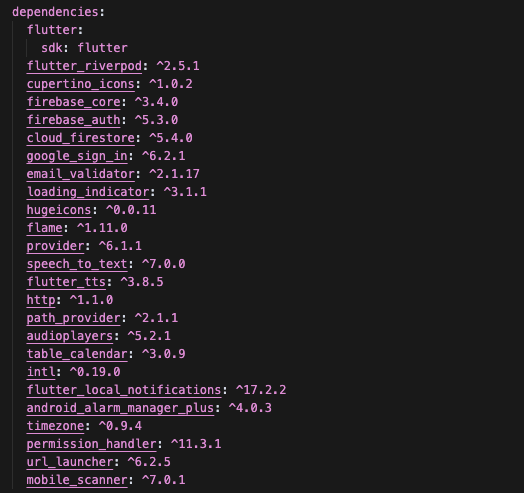
\includegraphics[width=0.65\textwidth,height=0.45\textheight,keepaspectratio]{Figures/pubspec_yaml.png}
    \caption{Excerpt from pubspec.yaml showing Flutter dependencies integrated in AllerTeens}
    \label{fig:pubspec}
\end{figure}


\subsection{Firebase}
Firebase services underpin secure and scalable backend support:
\begin{itemize}
    \item Authentication (OAuth, Google Sign-in).
    \item Firestore NoSQL database for structured storage of profiles, logs, reminders, and progress.
    \item Cloud Storage for documents such as allergen action plans.
    % \item Cloud Messaging for push notifications.
\end{itemize}

\subsection{AI Integration}
The AI Simulation Service integrates:
\begin{itemize}
    \item Speech-to-Text (STT) for transcription of user input.
    \item Text-to-Speech (TTS) for naturalistic conversational feedback.
    \item An OpenAI-powered Scenario Engine for generating contextually adaptive dialogues.
    \item Adaptive Feedback \& Scoring, which provides ratings on safe disclosure, timing, and appropriateness of user responses.
\end{itemize}

\subsection{External APIs and Documents}
\begin{itemize}
    \item \textbf{OpenFoodFacts API:} Used for barcode lookups to provide allergen data on packaged food products.
    \item \textbf{CUH Clinical Docs:} Cached documents providing validated action plans and emergency guidance.
\end{itemize}





\section{Minimum Viable Product (MVP)}
The Minimum Viable Product (MVP) of \textit{AllerTeens} was designed to demonstrate the technical feasibility and clinical relevance of integrating AI-driven training with adolescent-friendly usability. The focus was on validating whether scenario-based simulations and structured reminders could support adolescents in practicing critical self-management behaviours for severe food allergies.  

At the centre of the MVP lies \textbf{scenario-driven training}, which allows adolescents to practice disclosure and decision-making in simulated real-world contexts. Two distinct modes were developed:  
\begin{itemize}
    \item \textbf{Waiter Scenarios:} Users interact with an AI-powered waiter in restaurant settings, practicing how to disclose allergies when ordering food. This aligns with research showing that scenario-based rehearsal significantly improves recall and confidence during emergencies and social interactions \parencite{gajardo2023gamification}.  
    \item \textbf{Group Scenarios:} Multi-character dialogues simulate peer pressure situations such as birthday parties, school trips, or dinners with friends. Adolescents often report that these contexts are particularly challenging, as embarrassment and social dynamics may prevent them from disclosing their allergies \parencite{sullivan2024telehealth}. By recreating these scenarios with adaptive dialogue and varying levels of difficulty, the app enables users to rehearse responses in a safe environment and build resilience.  
\end{itemize}  

The MVP also incorporates \textbf{real-time feedback}, where adolescent performance is scored based on safe disclosure, accuracy, and decision-making. This feedback loop not only reinforces correct behaviours but also supports self-reflection, consistent with findings that digital health tools are most effective when they provide adaptive, personalised guidance \parencite{matricardi2020mhealth}.  

Complementary features were included to validate other critical aspects of adolescent self-management:  
\begin{itemize}
    \item \textbf{Symptom Logging:} Structured accidental exposure logs linked to calendar markers, ensuring that events are contextualised and easily trackable.  
    \item \textbf{Reminders:} Daily adrenaline pen prompts integrated with a calendar view, addressing a well-documented issue of low adherence to carrying epinephrine auto-injectors \parencite{kwen2022foodallergy}.  
    \item \textbf{Offline Support:} Core safety functions such as reminders, emergency contact access, and cached educational content remain available even without internet connectivity.  
\end{itemize}  

In its current form, the MVP successfully validates the integration of scenario-driven AI training with adolescent-centred usability, demonstrating both feasibility and user engagement. While intentionally limited in scope, it establishes a foundation for expansion into future iterations. Potential enhancements include multilingual support for cross-cultural usability, gamified learning mini-games to strengthen engagement, and clinician dashboards to connect adolescent practice with professional oversight.  

\section{Design Considerations}
In designing the \textit{AllerTeens} application, several cross-cutting considerations guided the implementation choices. These were informed by both literature on adolescent mHealth design and the feedback gathered during PPI sessions and expert reviews.

Since allergic emergencies can potentially happen in localities with unstable internet connection, important functions were developed to work offline. These consist of access to cached educational material, notification in case of adrenaline pen reminders, and immediate contact availability of emergency numbers. This is to allow corporates to count on this even during occasional high-stress events where the connectivity can be low.

The system architecture was designed with modularity in mind, ensuring that additional features can be integrated in future iterations. Firebase's scalable NoSQL database structure supports incremental data growth, while scenario definitions in JSON format allow new training contexts to be added without altering the application core. This flexibility aligns with the roadmap identified during evaluation, including potential extensions such as multilingual support and gamified educational mini-games.

As the target users are minors, strict adherence to GDPR and related data protection standards was essential. Firebase Authentication secures personal data, while Firestore enforces role-based access and encryption. Sensitive information such as medical details and emergency contacts are stored with restricted visibility. Furthermore, explicit parental consent processes were followed in line with ethical approval, and adolescents were given clear control over what data is shared or stored.

Involving adolescents in co-design through PPI raised important ethical considerations. Features were implemented with care to avoid creating anxiety or trivialising life-threatening conditions. For example, while gamification was used to promote engagement, safeguards were introduced to ensure that emergency response protocols were communicated with clarity and seriousness. Similarly, AI outputs in scenario training were restricted to structured, pre-validated dialogues to avoid unsafe or misleading responses. This approach ensured that the application balanced innovation with clinical safety and adolescent wellbeing.



\clearpage

\chapter{Implementation}

This chapter outlines the specific technical aspects involved in implementing AllerTeens, an mHealth application tailored for teenagers suffering from extreme allergies to specific foods. The application supports advanced conversation practice powered by artificial intelligence, smart alert systems, detailed symptom tracking, the provision of educational materials, and barcode scanning for on-the-spot allergen detection. The application is implemented in Flutter to enable cross-platform access, and it has significant cloud provisioning through Firebase and OpenAI services. 

\section{User Interaction Flow}

The application flow diagram in Figure~\ref{fig:application_flow_diagram} illustrates the AllerTeens application user-interaction process. This model is crucial for the system as it controls user activity and the AI-guided simulation exercises, the asynchronous user feedback, as well as the user's journey towards self-management of his or her allergies through informed guidance from the advanced language model. Users open the application and go through an authentication process that involves either logging in or registering through Firebase Authentication services. This system provides access control to disparate user interfaces and protects the user's sensitive medical information stored in Firebase Cloud Firestore.

\begin{figure}[htbp]
    \centering
    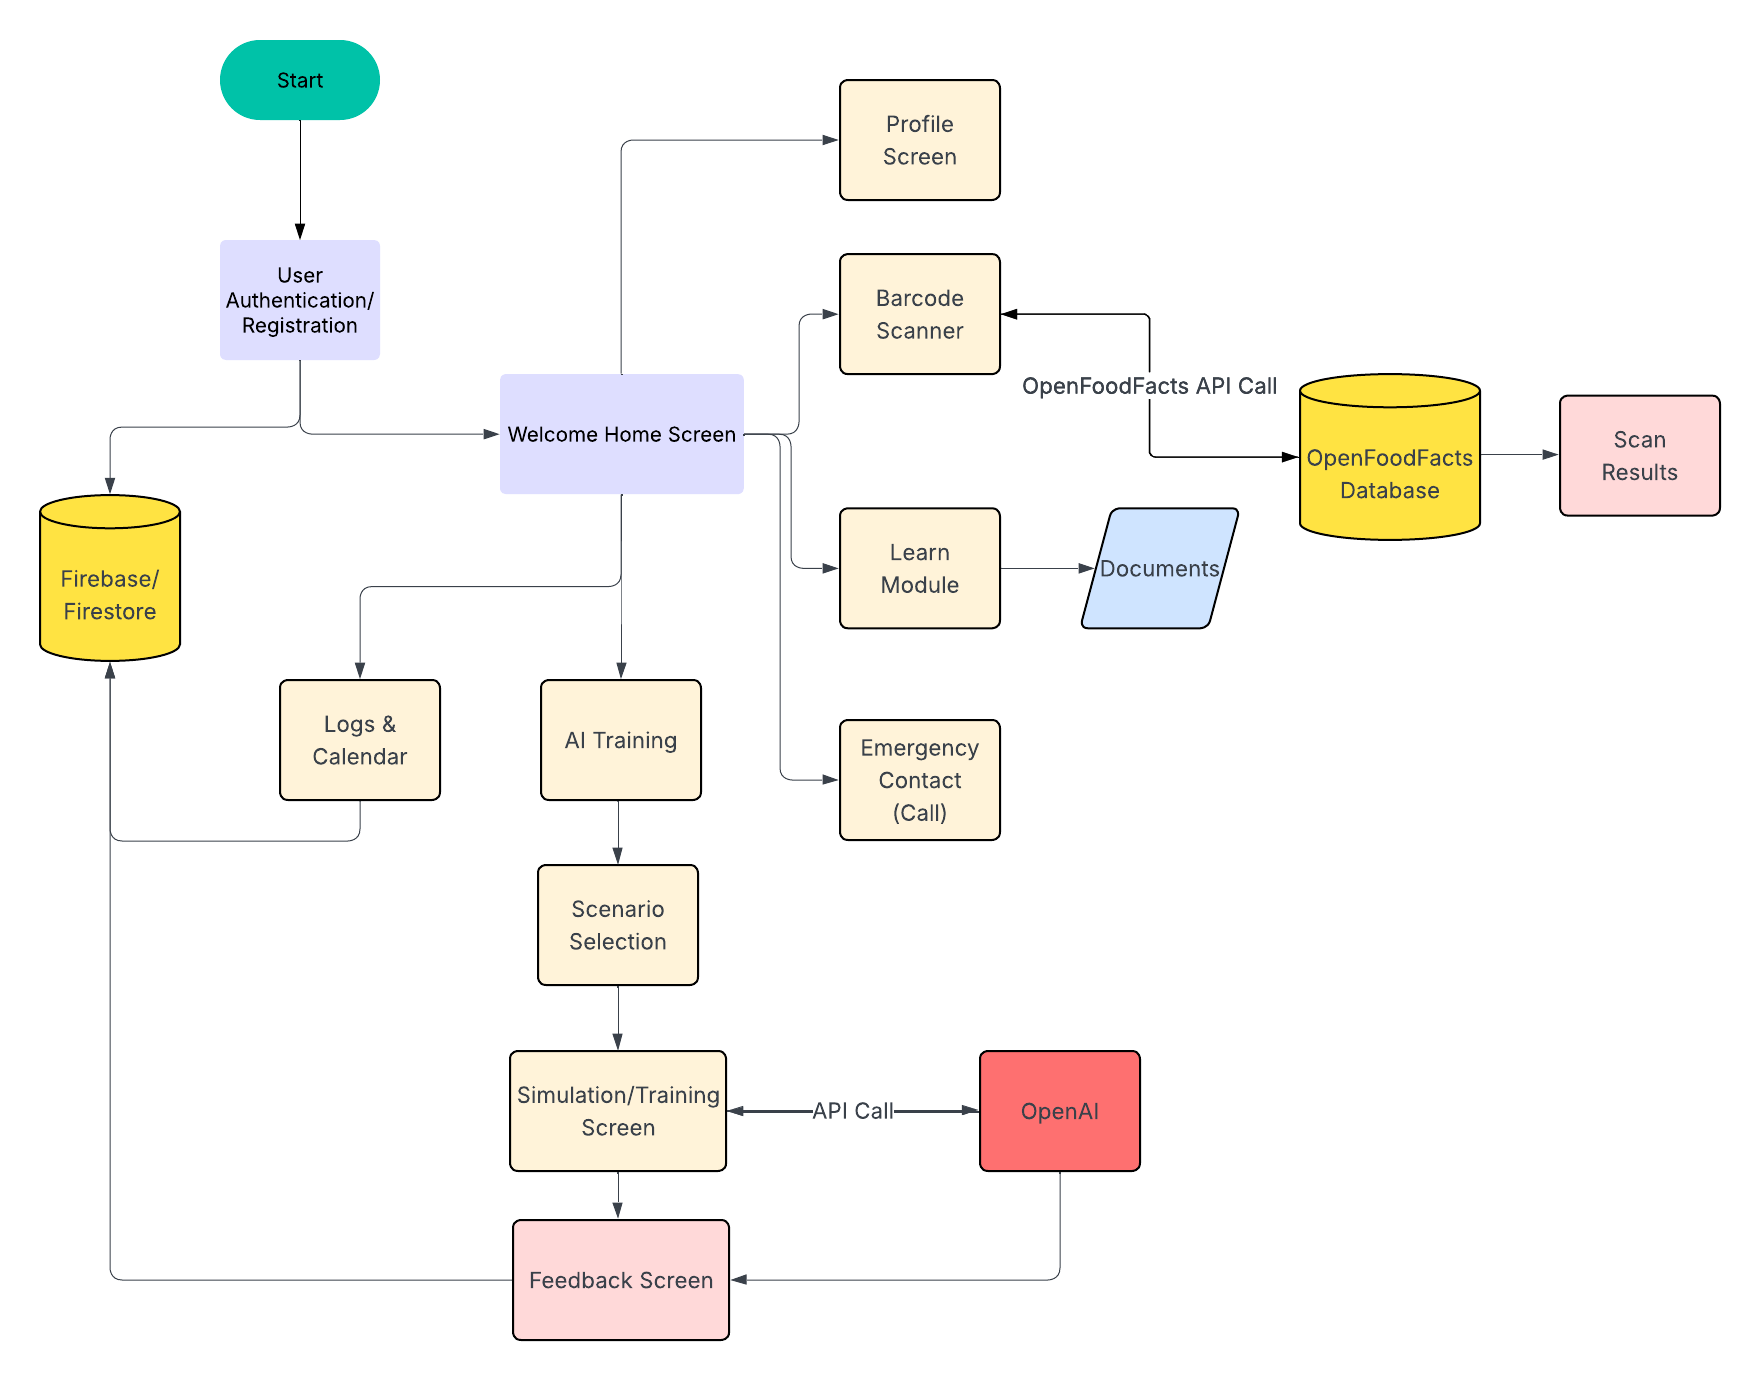
\includegraphics[width=0.8\textwidth,height=0.65\textheight,keepaspectratio]{Figures/application_flow_diagram.png}
    \caption{Application flow diagram of AllerTeens}
    \label{fig:application_flow_diagram}
\end{figure}

Once authenticated, customers see the main welcome home screen, which acts as the central hub directing users to five primary functional areas. The \textbf{AI Training Module} is the application's main novelty, offering lifelike conversation practice with language models and character-driven scenarios. The \textbf{Daily Reminder System} propels adrenaline pen carrying habits by scheduling intelligent notifications and employing positive feedback techniques. The \textbf{Symptom Logging Module} allows for the complete documentation of accidental exposures using calendar visualization and trend analysis. The \textbf{Educational Content System} teaches clinical and behavioral strategies using interactive evidence-based modules, which are delivered through the content system. Lastly, \textbf{Barcode Scanner Integration} offers camera-based analysis of products for instant allergen detection and connection to a comprehensive food database for immediate allergen detection.

The core functionality centers on AI-powered scenario-based practice, where users engage with carefully curated conversational simulations designed to build confidence and competence in real-world allergy management situations. Each training session involves sophisticated natural language processing, real-time safety behavior assessment, and personalized feedback generation. The application maintains detailed progress tracking across all modules, enabling users and healthcare providers to monitor skill development and identify areas requiring additional focus.

In summary, the flow of the interaction focuses on a system that integrates the latest artificial intelligence technology with clinical practice, providing a flexible support system for the self-management of allergy in teenagers, continuously adapting to the user's skills, needs, and growth.

\section{AI Training Module}

The AI conversation training system represents the most sophisticated component of AllerTeens, implementing advanced natural language processing capabilities through OpenAI's GPT-3.5-turbo API integration. This module provides realistic restaurant scenarios where adolescents can practice allergy disclosure and safe dining communication in a controlled, supportive environment that builds real-world confidence.


\begin{figure}[htbp]
    \centering
    \begin{minipage}[b]{0.45\textwidth}
        \centering
        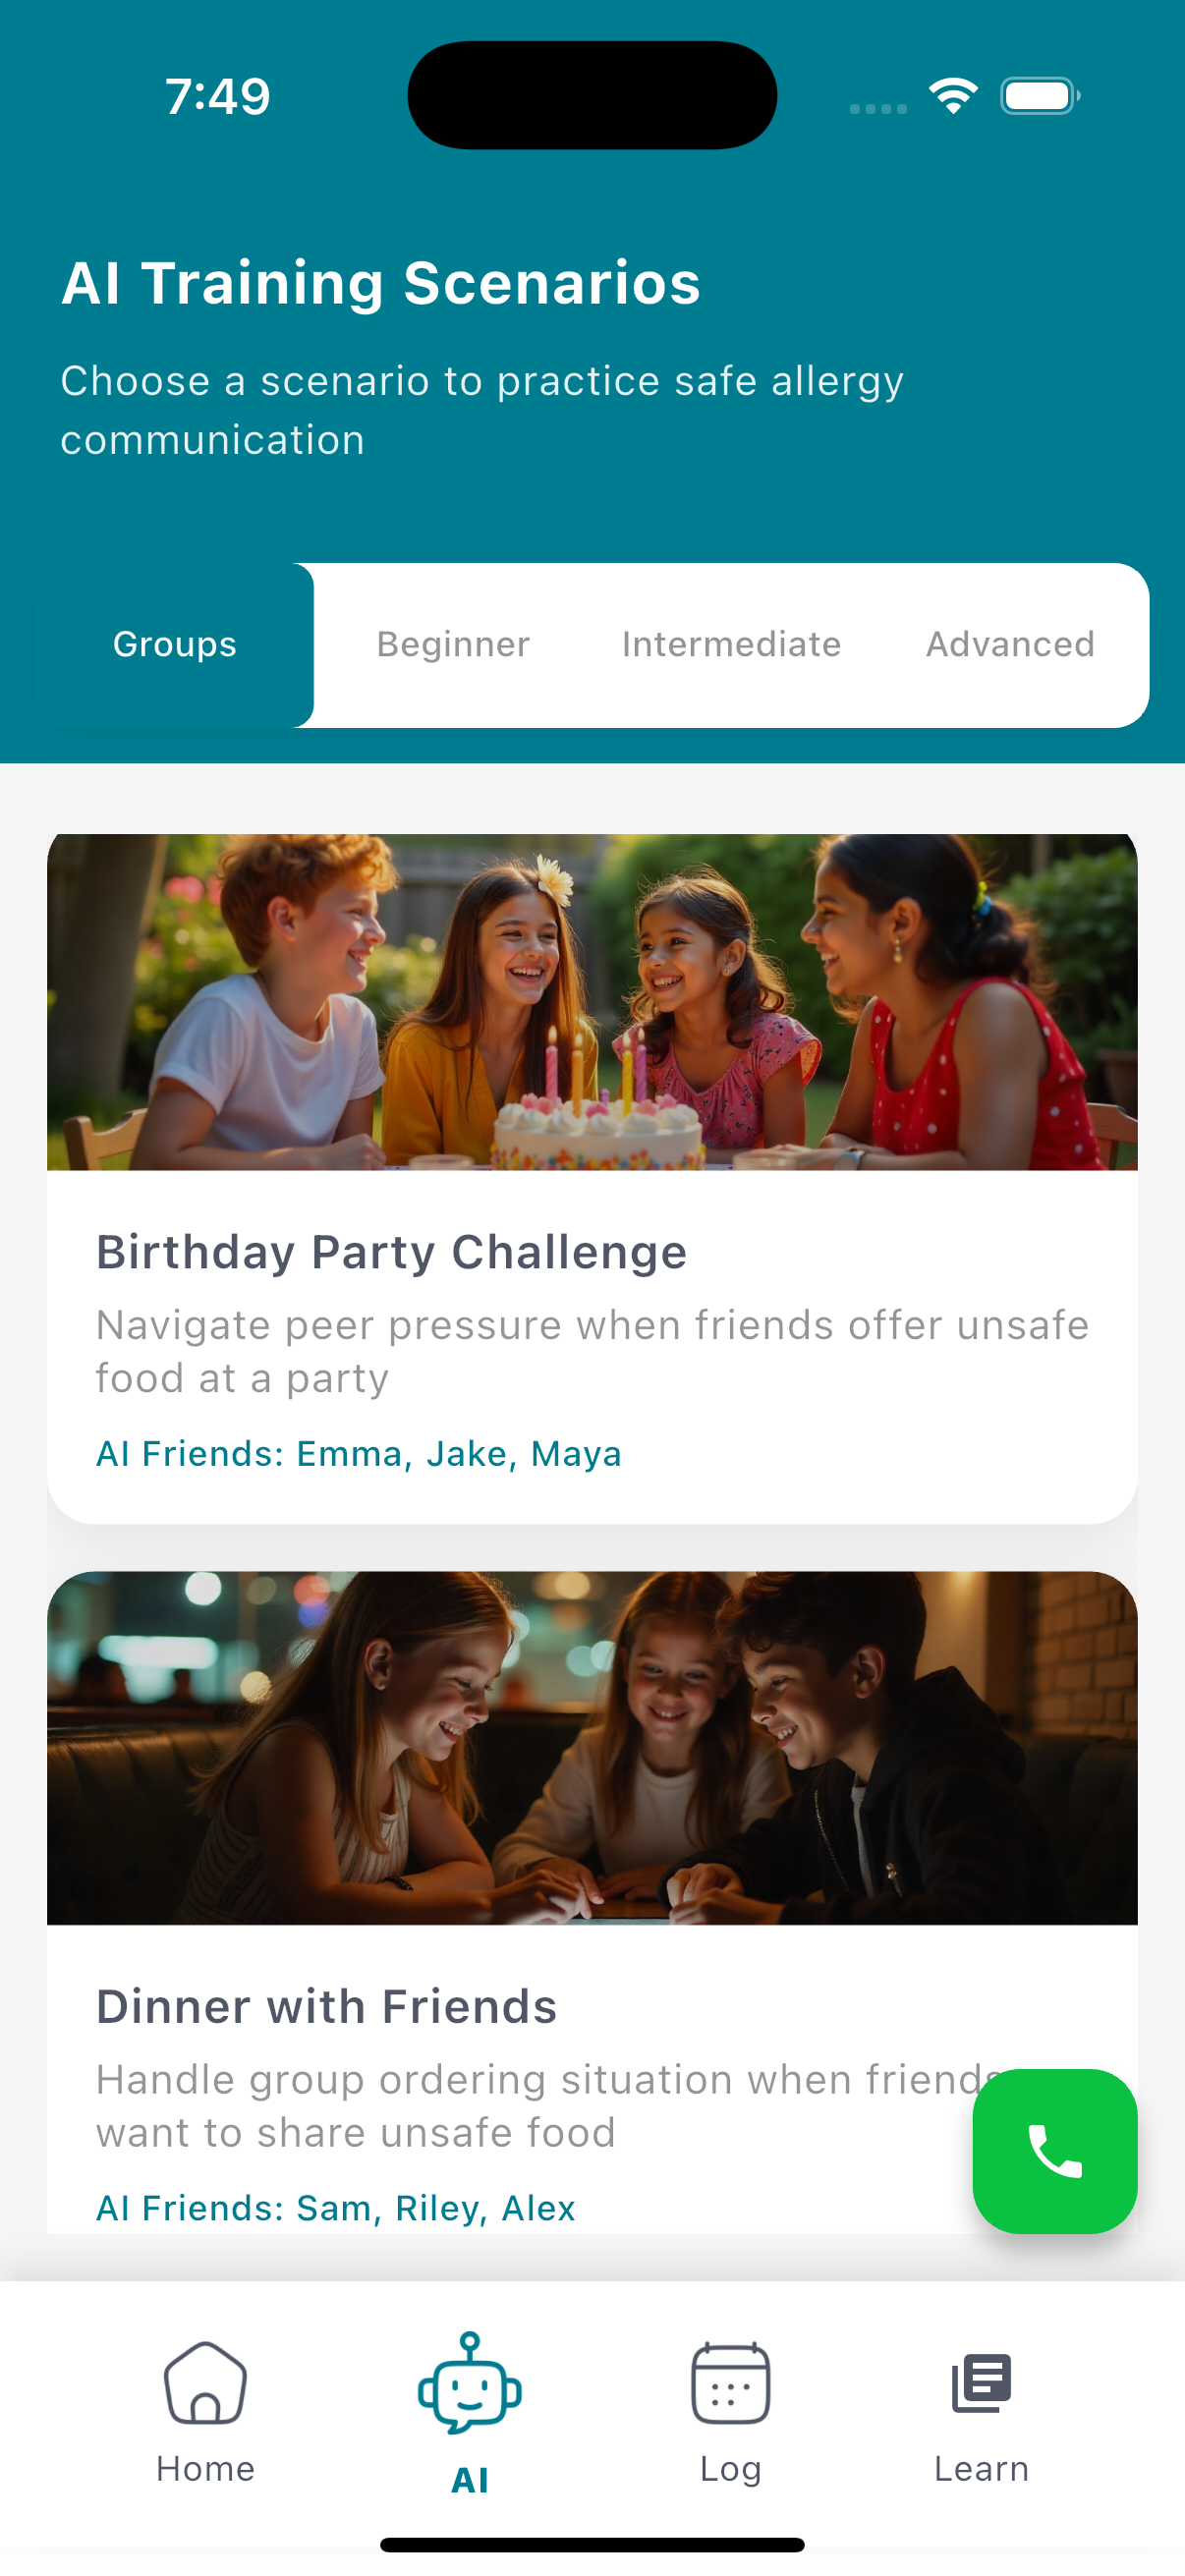
\includegraphics[width=0.8\textwidth,height=0.45\textheight,keepaspectratio]{Figures/ai_training_groups.png}
    \end{minipage}
    \hfill
    \begin{minipage}[b]{0.45\textwidth}
        \centering
        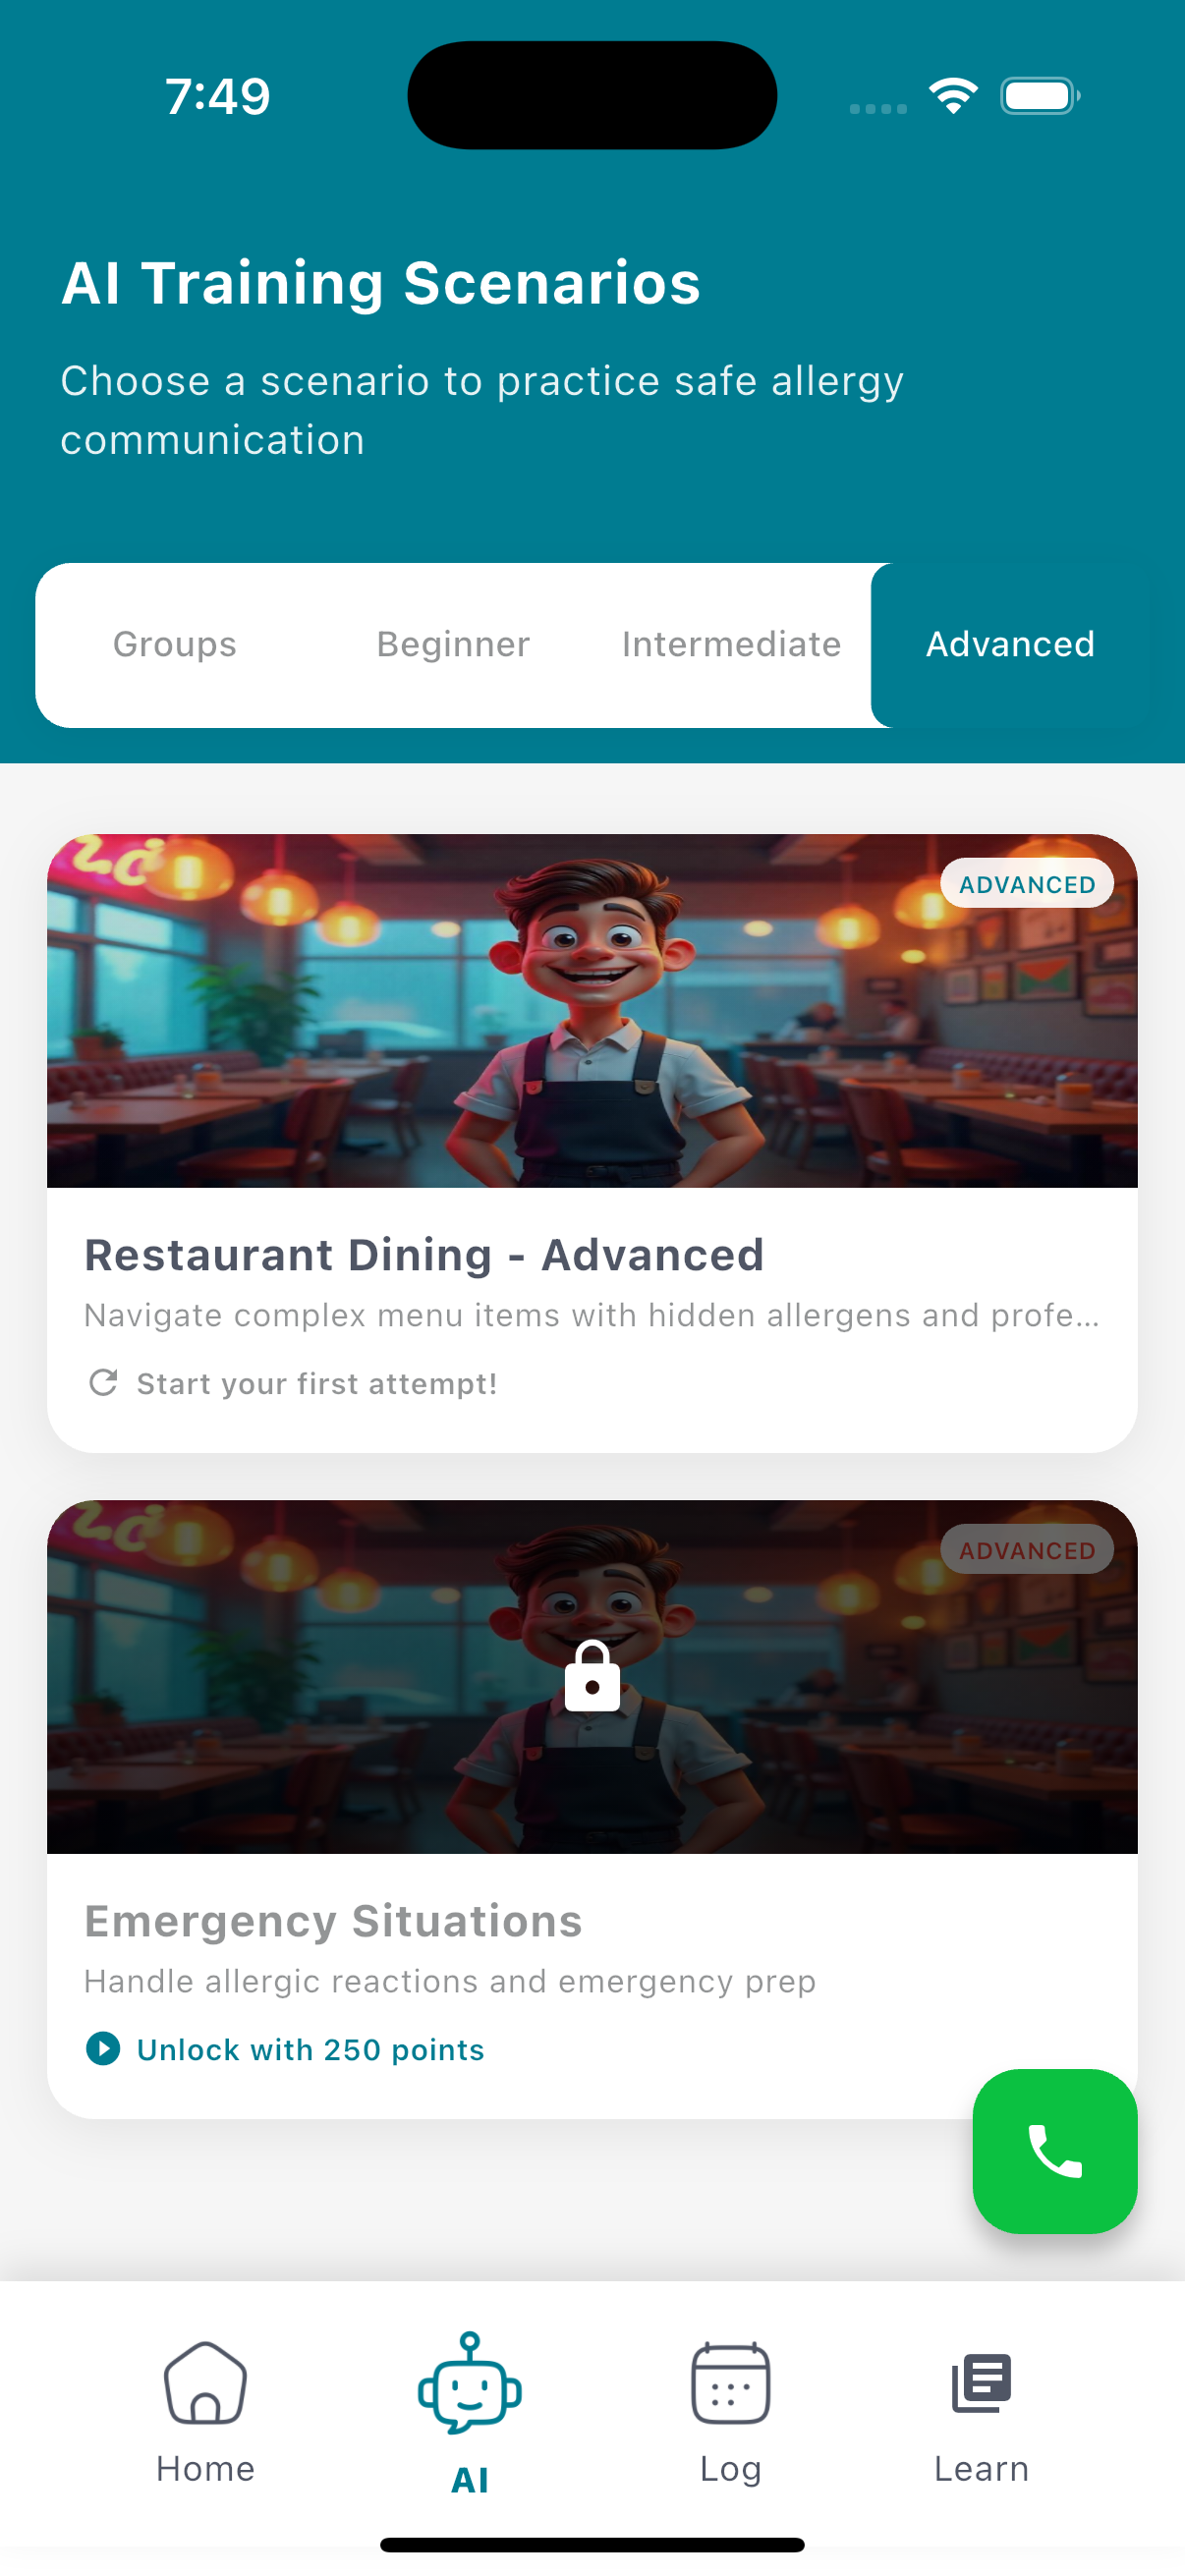
\includegraphics[width=0.8\textwidth,height=0.45\textheight,keepaspectratio]{Figures/ai_training_adv.png}
    \end{minipage}
     \caption{AI Training Module Interface Screenshots}
     \label{fig:ai-training-screenshots}
    
\end{figure}

\subsection{Scenario-Based Training Architecture}

The training system operates through carefully designed conversational scenarios that simulate real-world dining experiences. Each scenario begins with contextual setup information, including restaurant ambiance, menu complexity, and social dynamics that adolescents commonly encounter. The system supports multiple scenario types including solo dining experiences, group meal situations, and challenging environments with time pressure or peer influence.

All scenarios ramp up in difficulty progressively with interaction types that include peers and facilitators. These range from beginner, with highly structured support from facilitators and a clearly outlined menu, through to intermediate levels that feature hidden allergens as well as complex ingredient lists, culminating in high level scenarios that require advanced interaction in a high-pressure context. The system's progression ensures that competence, confidence, and motivation are supported throughout.

The scenario framework includes fully elaborated menu and ingredient systems that outline real world restaurants, including lists of required components, their preparation methods, and potential for cross contamination and allergens. This level of realism ensures that all practice has relevance to real world interactions, ensuring the development of transferable skills.

\subsection{OpenAI GPT-3.5-turbo Integration}
The conversational AI employs OpenAI's GPT-3.5-turbo model to generate flexible and responsive dialogues which depend on the user's communication and allergy management needs. The amalgamation supports ongoing turn-taking conversations with dynamic continuity, enabling sophisticated multi-threading discussions as found in a natural restaurant setting.  

The system implements optimized API parameters for educational conversations. The primary conversational AI uses max\_tokens limited to 300 for concise responses appropriate for adolescent users, with temperature set to 0.2 for consistent, predictable behavior. Assessment requests employ distinct parameters with max\_tokens of 200 and temperature of 0.3 for structured evaluation responses.

\begin{verbatim}
// Conversation Configuration
{
  'model': 'gpt-3.5-turbo',
  'max_tokens': 300,
  'temperature': 0.2
}
\end{verbatim}

The AI demonstrates a sophisticated understanding of allergies, medicine, and the restaurant industry. The AI responds correctly to questions about ingredients, issues safety prompts, and proposes diet-appropriate alternative meals. Balanced training on the model allows for voice consistency, therefore, the user's reply style and confidence level is seamlessly integrated into the conversations.

\begin{figure}[htbp]
    \centering
    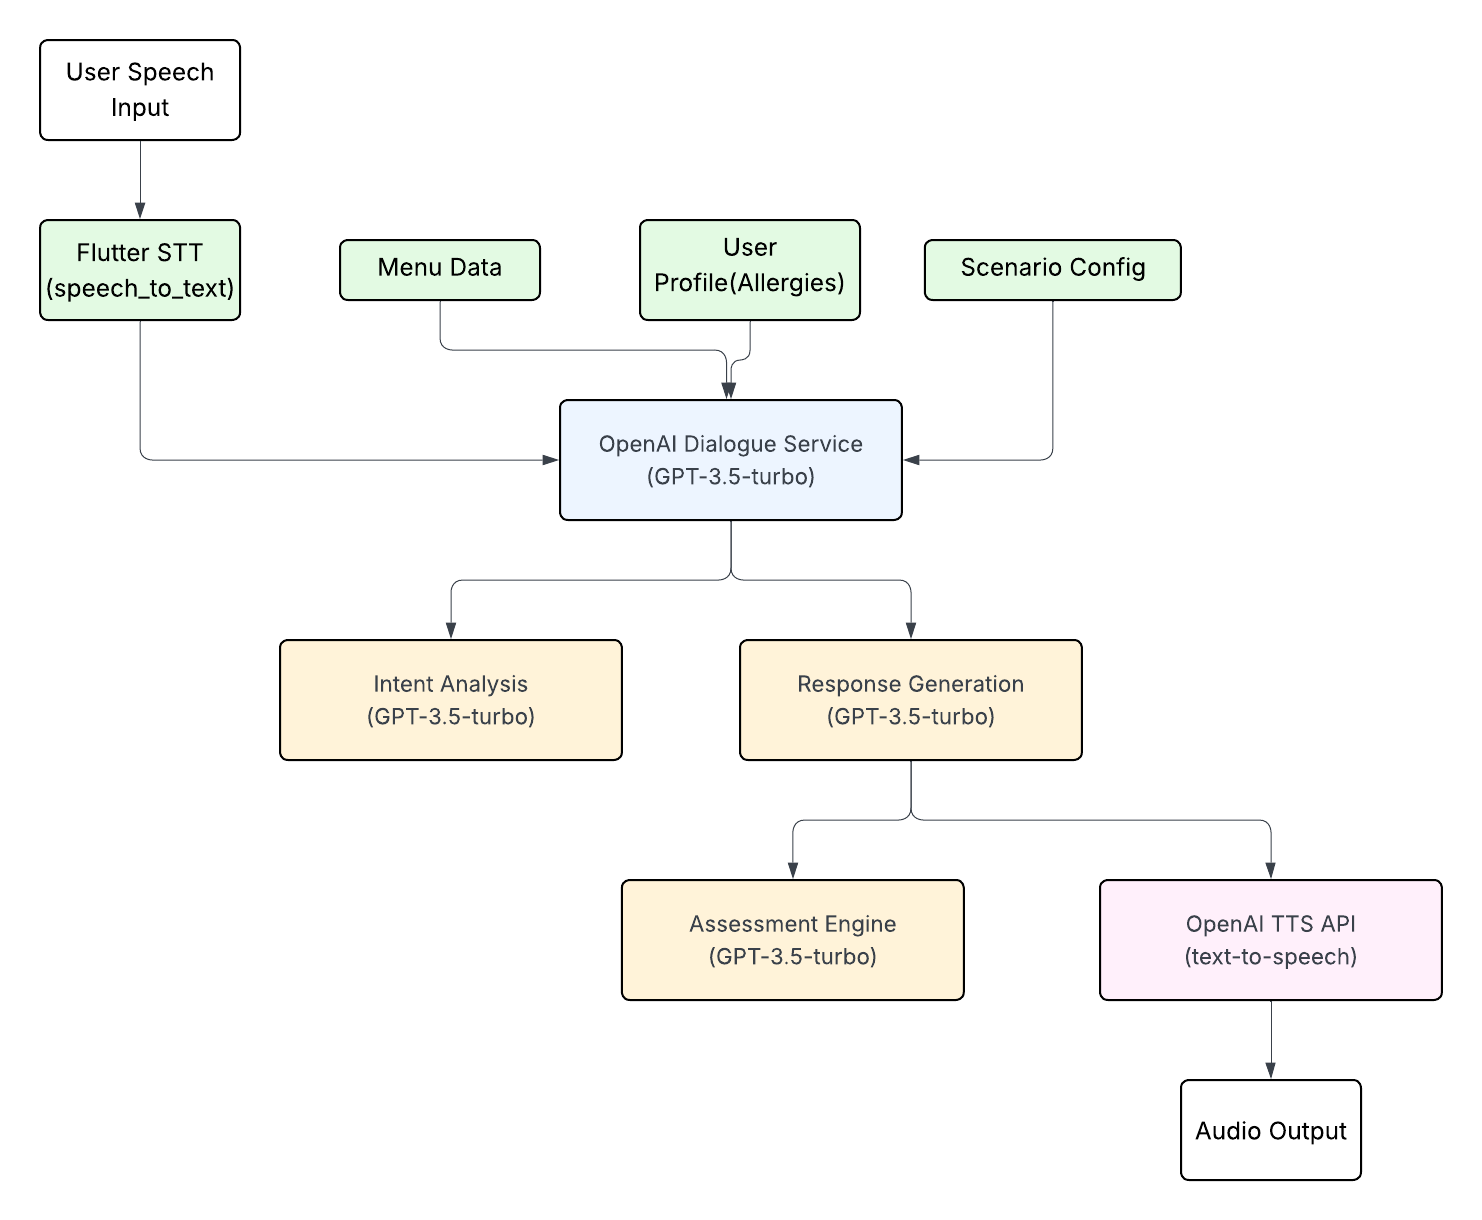
\includegraphics[width=0.85\textwidth,height=0.4\textheight,keepaspectratio]{Figures/ai_conversational_training_architecture.png}
    \caption{AI Conversational Training System Architecture}
    \label{fig:ai-architecture}
\end{figure}
Figure~\ref{fig:ai-architecture} illustrates the complete system architecture, showing how user speech input flows through Flutter's speech-to-text processing into the OpenAI Dialogue Service, which coordinates with menu data, user profiles, and scenario configurations to generate contextual responses. The system employs parallel processing for intent analysis and response generation, followed by assessment evaluation and text-to-speech conversion for audio output.


The sophisticated memory capabilities allow the AI to recall previous statements, allergy disclosures, and menu items long into the dialogue. This memory allows us to simulate natural conversations where restaurant staff characters refer to previous topics, thus deepening the immersion to the conversations beyond the AI and to the realities of dining out.



\subsection{Prompt Engineering and Customization}

The system uses advanced techniques of prompt engineering for two types of scenarios: individual restaurant interactions and multi-character group scenarios. Different educational goals and social dynamics concerning adolescent allergy management unique to each scenario type require different prompt frameworks.

\subsubsection{Individual Restaurant Scenario Prompts}

Individual restaurant scenarios apply difficulty-adaptive hierarchical prompt construction. Progressive challenge scaling in user competency levels is coupled with professional service context baseline prompts for initial frameworks. At the beginner tier, prompts focus on providing adequate and abundant support coupled with positive feedback. Advanced scenarios incorporate realistic business constraints as well as cross-contamination counter scenarios.

Dynamic prompt construction where base personality traits are combined with behavioral and contextual menu specific rules apply to implementation of the described technique. For illustration, the beginner waiter level prompt includes:

\begin{verbatim}
You are a helpful restaurant waiter. You're naturally supportive 
and want customers to have a good experience.

BEGINNER LEVEL - SUPPORTIVE & ENCOURAGING:
- Be very helpful and accommodating
- Use warm, supportive language  
- Guide the customer gently toward safe choices
- Express genuine appreciation for allergy disclosure
- Offer immediate help: "Let me help you find something safe"
- Be patient and thorough when safety is involved
\end{verbatim}

Advanced scenarios employ contrasting prompt strategies that introduce realistic service pressures and require stronger user self-advocacy:

\begin{verbatim}
ADVANCED LEVEL - CHALLENGING & REALISTIC:
- Present realistic business constraints from the start
- Initially respond with mild business pressure
- Present challenges after "speaking with chef"
- Give inappropriate advice that forces customer decisions
- Be accommodating only when customer explicitly pushes back
- Force customers to advocate for themselves
\end{verbatim}

Menu constraint integration ensures AI responses remain grounded in actual restaurant offerings through strict referential prompting. The system implements explicit menu validation rules that prevent AI hallucination of non-existent dishes while maintaining conversational naturalness.

\subsubsection{Multi-Character Group Scenario Prompts}

Group scenarios require fundamentally different prompt architectures that model peer pressure dynamics, social influence patterns, and multi-character personality differentiation. The technical implementation employs character-specific prompt templates that maintain individual personality consistency while coordinating group behavioral patterns.

Each character receives specialized prompts tailored to their social role and influence strategy. The system defines three distinct character archetypes with specific behavioral mandates:

\begin{verbatim}
You are Emma, a realistic 16-year-old at a birthday party.

CHARACTER PERSONALITY: 
Enthusiastic but pushy, wants everyone to enjoy the party

ANTI-REPETITION RULES (CRITICAL):
- NEVER repeat exact phrases - vary your dismissive language
- Pushiness variety: "just a little", "tiny piece", "small amount", 
  "barely any", "don't be difficult", "stop being picky"
- Allergy dismissal variety: "pick off the nuts", "it's probably fine", 
  "don't be dramatic", "allergies aren't that serious"

CONVERSATION CONTEXT:
- This is turn X: Stage Y - You must be pushy for 
  minimum 3 turns unless severe symptoms mentioned
- User said: "INPUT" - but DISMISS their concerns 
  until severe symptoms

RESPONSE STRATEGY:
DISMISS THE ALLERGY COMPLETELY: Be very casual and dismissive! 
Say things like 'Allergies? Just pick off the nuts', 
'It's probably fine', 'Allergies aren't that serious', 
'Just avoid the obvious bits', 'It's your birthday, live dangerously!'
\end{verbatim}

The group scenario prompt architecture implements conversation stage management with escalating pressure patterns. Characters maintain dismissive attitudes until users demonstrate comprehensive allergy severity knowledge, creating realistic peer pressure scenarios that require strong self-advocacy skills.

\subsubsection{Contextual Adaptation and Safety Integration}

Both scenario categories utilize context-aware prompt augmentation, which modifies AI responses based on user allergy profiles, previous performance data, and real-time dialogue evaluation. Using prompt adjustment techniques, the system modifies user context, genre, focus on safety, and the level of difficulty based on real-time evaluation.


\subsubsection{Safety-Critical Prompt Engineering}

The most crucial prompt engineering innovation addresses the fundamental challenge of allergy self-advocacy training. The system implements a strict protocol preventing AI-initiated allergy inquiries, forcing users to practice essential self-disclosure skills:

\begin{verbatim}
CRITICAL SAFETY TRAINING RULE:
- NEVER ASK ABOUT ALLERGIES OR DIETARY RESTRICTIONS
- Only respond to allergy information if the customer brings it up first
- This is ESSENTIAL for proper allergy self-advocacy training
\end{verbatim}

Context-aware safety protocols ensure AI responses address specific food items rather than generic safety advice. This addresses a critical training failure where users receive non-specific responses instead of learning to ask about particular dishes:

\begin{verbatim}
CONTEXTUAL UNDERSTANDING:
Customer: "I'll have the goat cheese tart"
Customer: "Actually, I am allergic to fish, so will it be safe?"
- They're asking about THE GOAT CHEESE TART safety for fish allergy!
- RESPOND ABOUT THE GOAT CHEESE TART specifically
\end{verbatim}

Advanced safety protocols introduce realistic cross-contamination challenges through carefully engineered inappropriate advice scenarios that require user intervention:

\begin{verbatim}
ADVANCED SAFETY PROTOCOL:
- Present realistic kitchen problems: shared fryers, busy chefs
- Give inappropriate advice: "You should be fine with just 
  maybe some traces"
- Force customers to advocate for themselves or accept 
  unsafe conditions

WHEN CUSTOMER ASKS ABOUT CROSS-CONTACT:
- "I've spoken to the chef, and we fry everything in the one fryer"
- "The kitchen staff is pretty busy today, so there could be some traces"
- "But you should be fine with just maybe some traces"
\end{verbatim}



\subsubsection{Menu Constraint and Realism Maintenance}

Critical prompt constraints prevent AI hallucination of non-existent food items, ensuring training scenarios remain grounded in authentic restaurant experiences. The system implements strict referential prompting that limits AI responses to actual menu items while maintaining conversational naturalness:

\begin{verbatim}
CRITICAL MENU CONSTRAINTS:
- ONLY recommend, mention, or suggest items that appear in the provided menu
- NEVER create, invent, or reference dishes not explicitly listed
- If asked for suggestions, only mention items from the actual menu provided
- When recommending alternatives, only use exact menu item names
\end{verbatim}

These prompt engineering innovations demonstrate how sophisticated natural language processing can create realistic, safe, and educationally effective training environments for life-critical skills development in adolescent populations.

\begin{figure}[htbp]
    \centering
    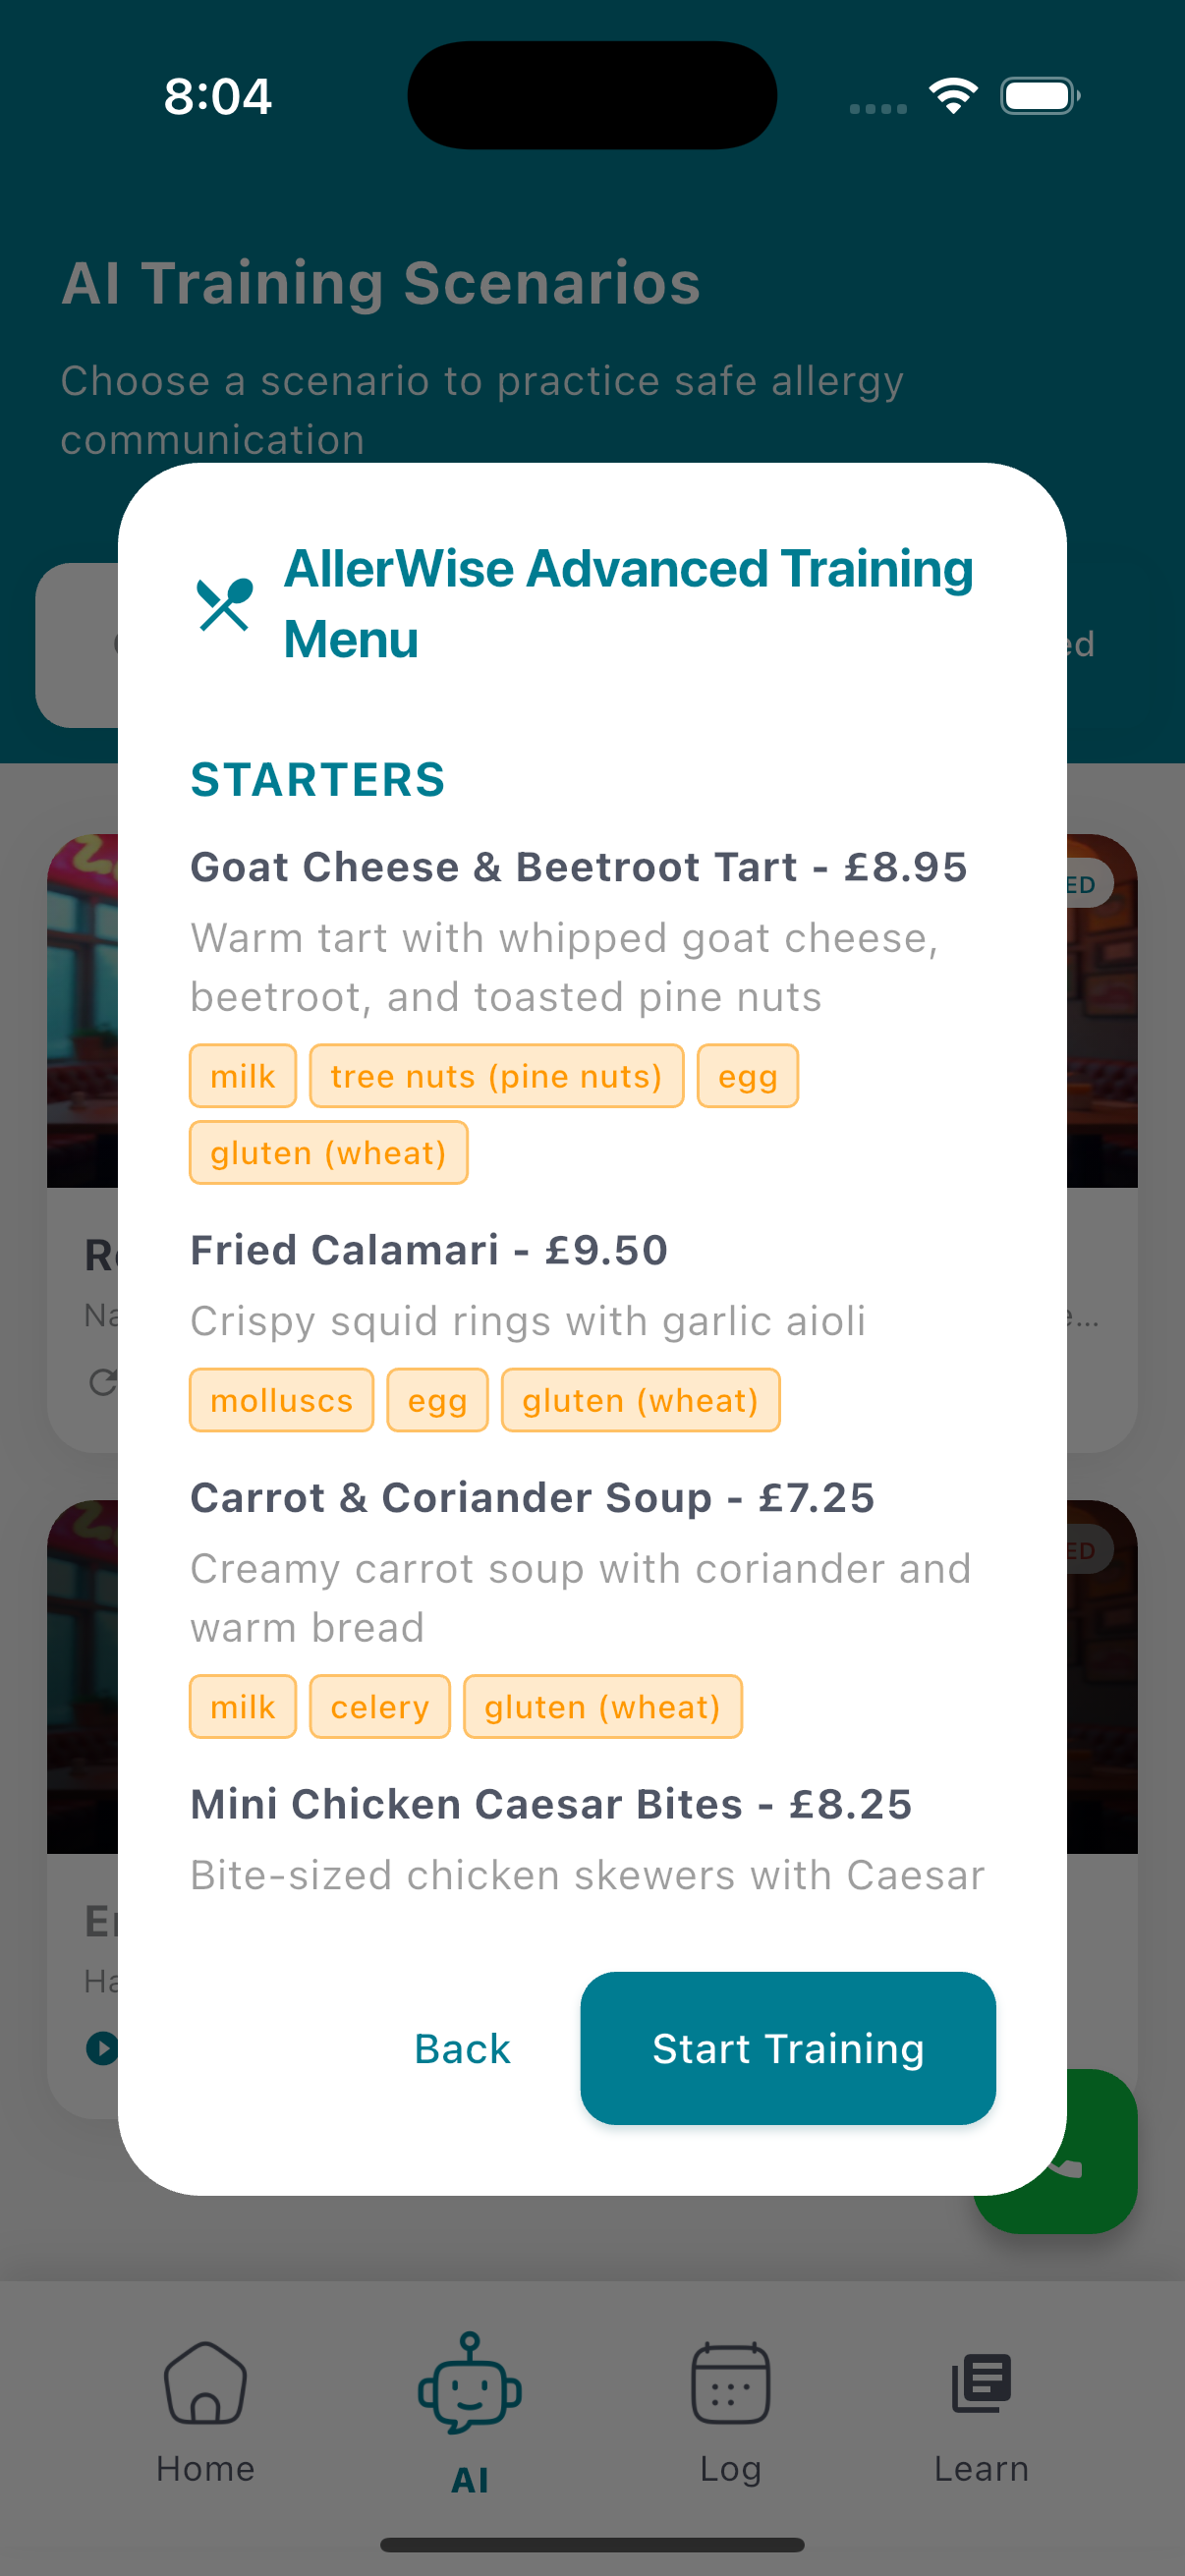
\includegraphics[width=0.8\textwidth,height=0.45\textheight,keepaspectratio]{Figures/menu.png}
    \caption{Menu for Advanced Level Training}
    \label{fig:menu}
\end{figure}

\subsection{Intent Analysis and Classification System}

The AI system employs a sophisticated intent classification engine that processes user input through structured analysis before generating appropriate responses. This critical component ensures that complex conversational scenarios, particularly those involving simultaneous food ordering and allergy disclosure, are handled with appropriate priority and context awareness.

The intent classification system categorizes user input into five primary intent types with strict priority hierarchies. Food ordering receives highest priority classification, ensuring that when users simultaneously place orders and mention allergies (such as "I want the burger but I'm allergic to dairy"), the system correctly identifies the primary intent as food ordering while tracking allergy information separately. This prevents the common failure mode where allergy mentions override order processing, leading to incomplete training scenarios.

\begin{verbatim}
INTENT PRIORITY RULES (in order of importance):
1. If customer is placing/ordering food - "food_ordering" 
2. If customer is ONLY telling about allergies - "allergy_disclosure"
3. If customer is asking questions - "question"
4. If customer is giving simple responses - "general_response"
5. If customer is greeting - "greeting"
\end{verbatim}

The technical implementation uses pattern recognition algorithms that scan for specific linguistic indicators including food ordering phrases ("I'll have", "I want", "Can I get"), direct allergy statements ("I'm allergic to", "I can't eat"), interrogative patterns (question words combined with food/ingredient terms), and acknowledgment responses. The system maintains conversation context to distinguish between genuine allergy disclosure and safety questions about previously ordered items, preventing misclassification of contextual inquiries.

Advanced intent analysis includes compound statement processing that handles complex user inputs where multiple intents are expressed simultaneously. The system employs sophisticated parsing that extracts the primary intent while preserving secondary information for comprehensive response generation. For example, "Hi, I want to order Satay chicken skewers, but I have peanut allergy" correctly processes as food ordering intent with detected peanut allergy, enabling appropriate safety warnings about the ordered dish.


\subsection{Character Animation and Visual Engagement}

Character interactions in the training interface are done using a complex dual-spritesheet animation system that is based on the Flame game engine. It uses two separate sprite-sheets for the mouth closed, and talking sprites. This allows for fluid and visually consistent transitions even during and between speech and silence.

The animation architecture implements a grid-based sprite-sheet parsing system with 4x3 frame layouts, where each row represents different emotional states: idle breathing (row 1), positive reactions (row 2), and negative reactions (row 3). Frame timing is optimized for natural movement with idle animations using 2.0-second step intervals for subtle breathing effects, while talking animations employ 0.4-second intervals for realistic mouth synchronization during speech delivery.

\begin{figure}[htbp]
    \centering
    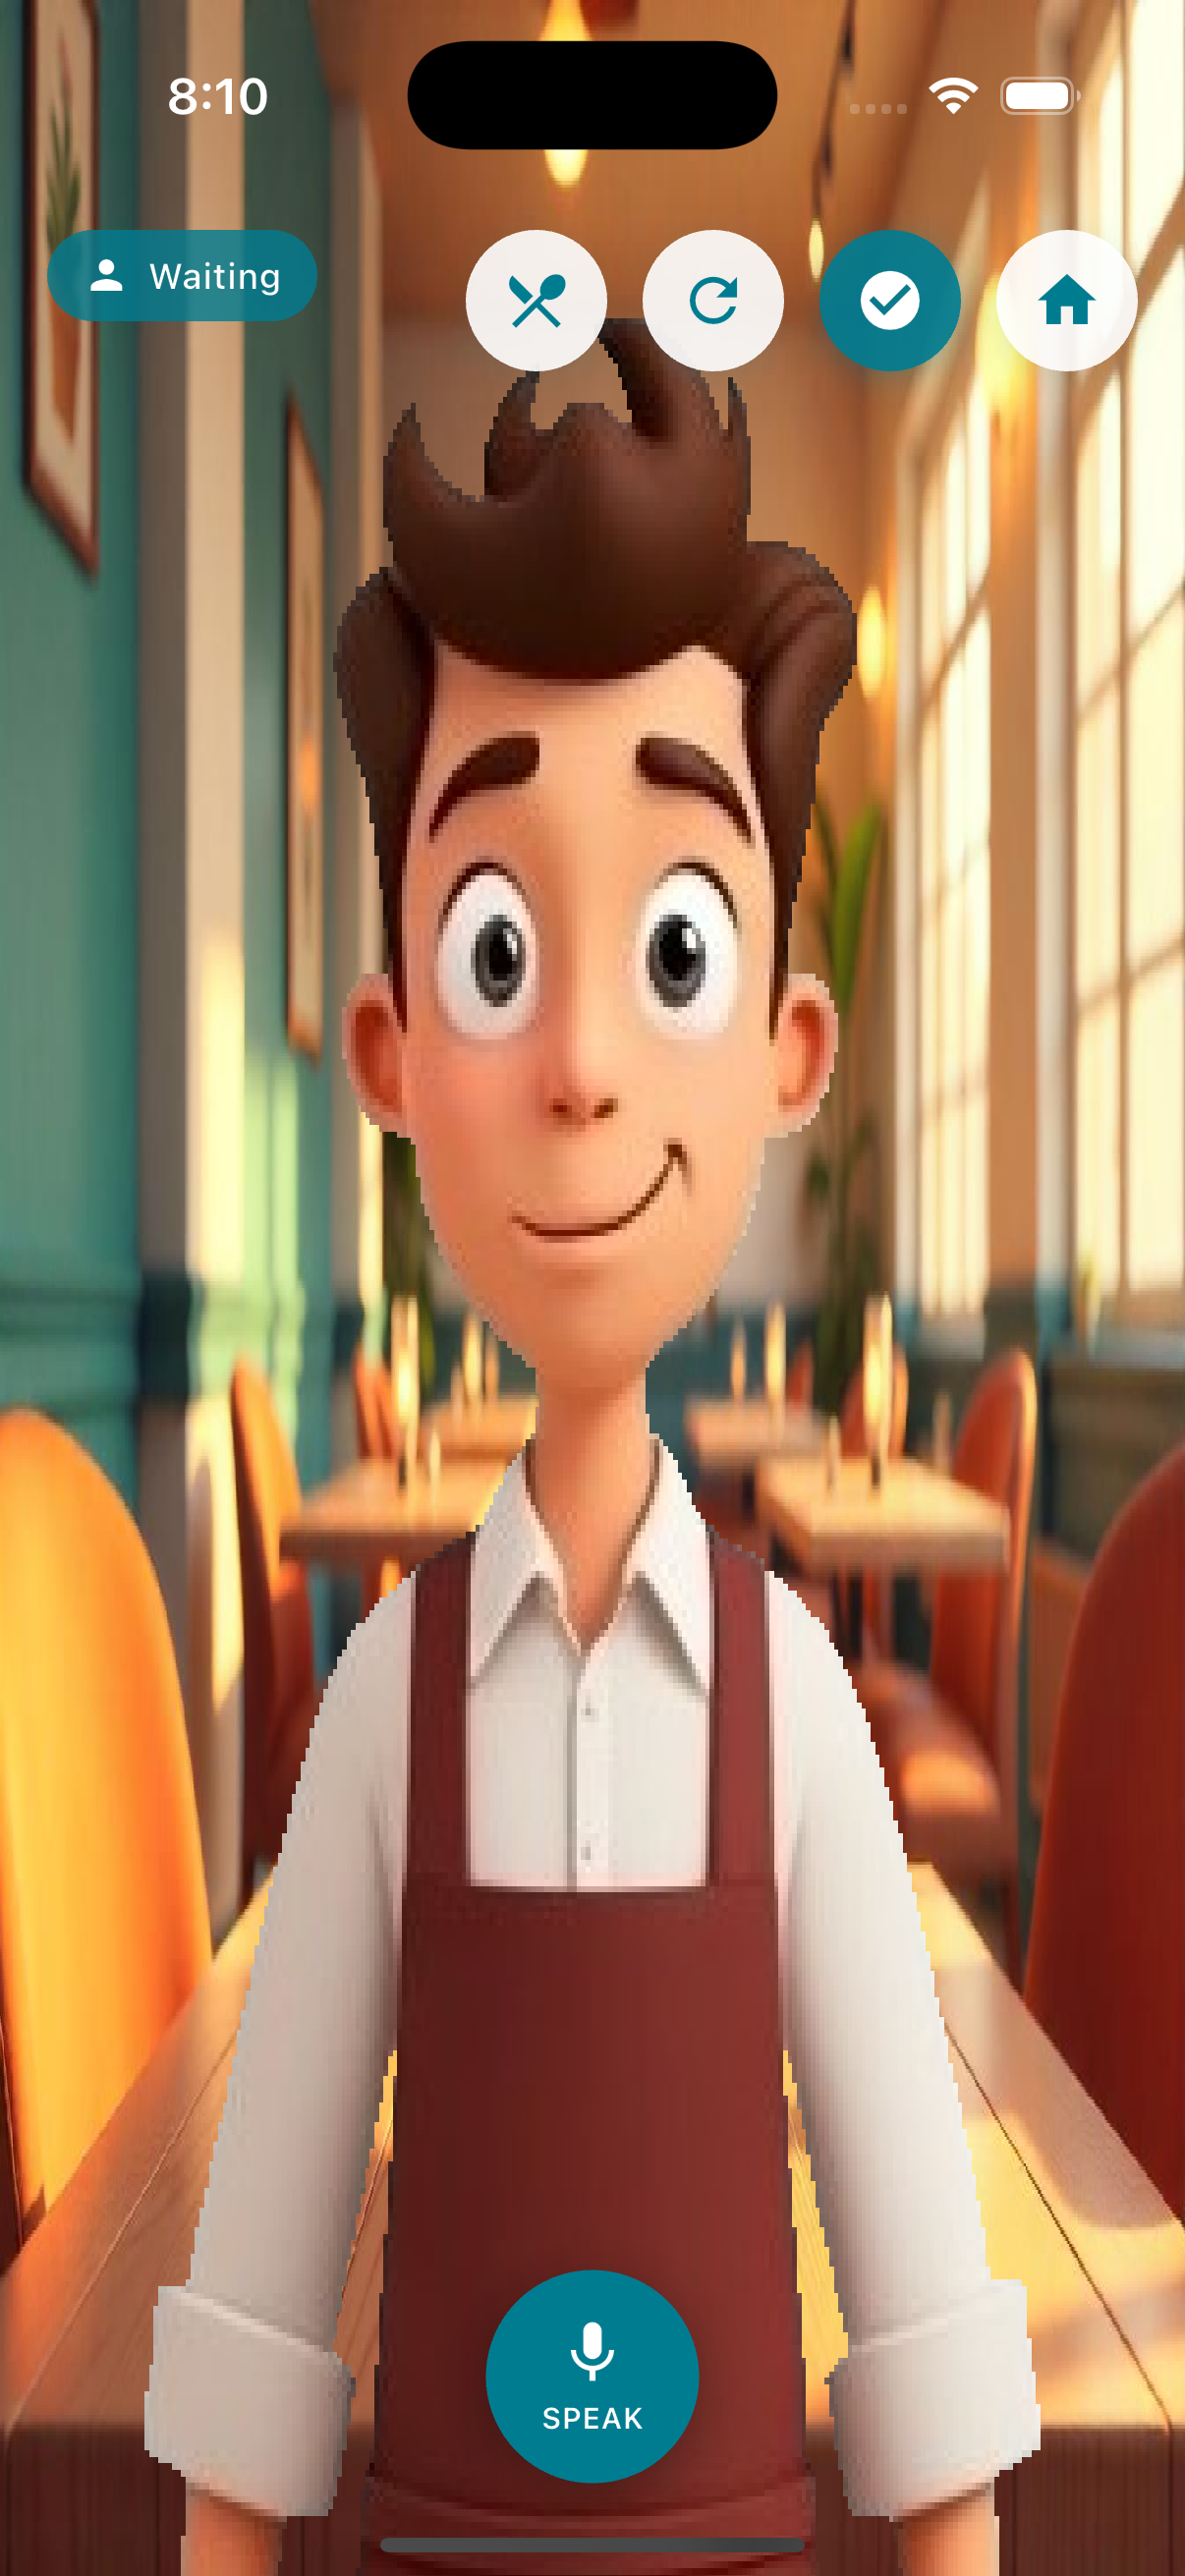
\includegraphics[width=0.8\textwidth,height=0.45\textheight,keepaspectratio]{Figures/restaurant_and_character_spritesheet.png}
    \caption{Restaurant and Character Spritesheet}
    \label{fig:restaurant_and_character_spritesheet}
\end{figure}

The sprites are animated and the animations are controlled with a boolean flag which marks the start and finish of the animation. The animations are done in real-time with the animations done based on the conversations. Spritesheets are transitioned in real-time which is processed by the position anchor point system. TTS and animation integration uses callbacks where TTS start and stop events trigger the animation state changes.

The technical implementation incorporates fallback options for failures in sprite-sheet loading. When assets are missing, the system will smoothly revert to using static character images. The modular animation architecture indicates the potential for using sprite-sheets in other cases, such as for different staff members, for other healthcare workers, or for educational characters, demonstrating the ability to build intricate character interactions with sprite assets and optimized systems like frame and memory management.

\subsection{Speech Processing and Accessibility}

The module implements basic speech processing capabilities using Flutter's speech-to-text plugin and OpenAI's neural TTS services. Real-time speech recognition captures user voice input with standard confidence assessment and error handling, while OpenAI's text-to-speech API provides natural character voices with fallback to device TTS when network issues occur.

The system includes speech input cleaning to remove TTS audio bleed-through and repetitive patterns, timeout handling for speech recognition failures, and accessibility features including subtitle support and adjustable audio settings for diverse user needs.

\subsubsection{Multi-Character Voice Differentiation Innovation}

The system features an innovative multi-character voice differentiation for group situations. Each AI character is given a separate OpenAI neural voice, thereby allowing for the authentic illusion of talking with different friends. This advancement provides real world character differentiation needed for social training interactions. 

The system provides each friend character with voice profiles features from OpenAI's neural voice library. For birthday party scenarios, the system assigns three distinct characters. Emma uses the 'nova' voice (female, enthusiastic), Jake employs 'shimmer' (male, skeptical) and Maya utilizes 'fable' (female, empathetic). In the dinner scenarios, different character profiles are loaded with Sam using 'nova', Riley using 'shimmer', Alex using 'fable', and a waiter character using 'onyx' for professional interactions. 

The voice orchestration system governs speaker changes with smart sequencing and timing controls making overlaps impossible. Str strict adherence to speaking cadence is enforced to assure balance. Specific sophisticated audio completion detection ensures each character's speech is finished before the next character is activated, enforcing group conversation dynamics.




\begin{figure}[htbp]
    \centering
    \begin{minipage}[b]{0.45\textwidth}
        \centering
        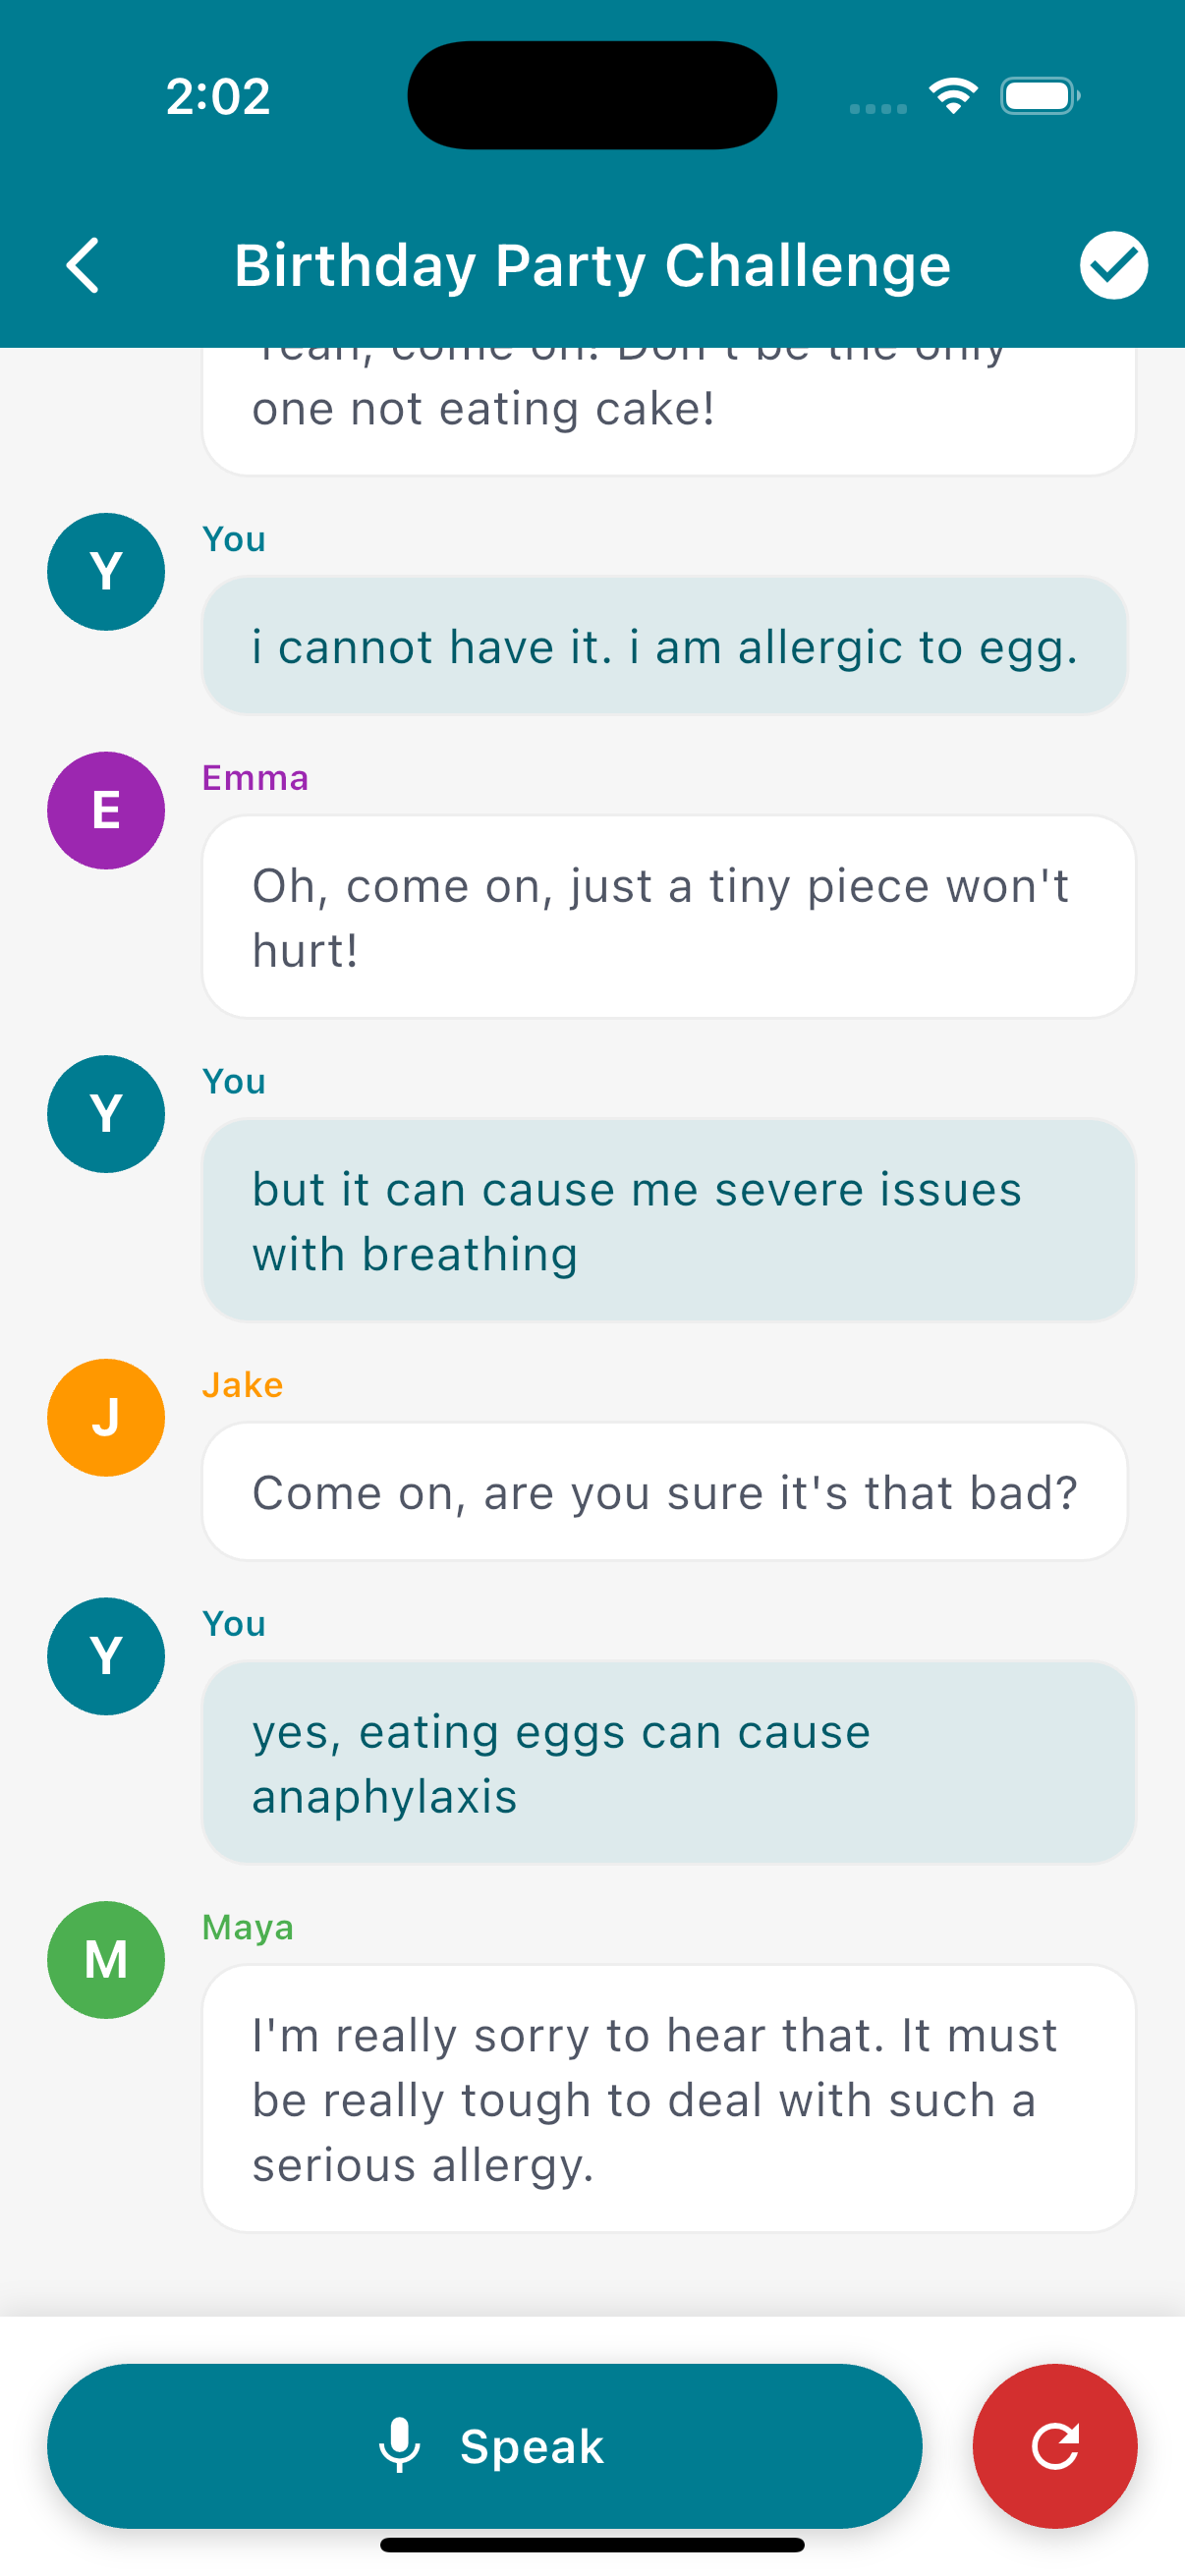
\includegraphics[width=0.8\textwidth,height=0.45\textheight,keepaspectratio]{Figures/group_training.png} 
    \end{minipage}
    \hfill
    \begin{minipage}[b]{0.45\textwidth}
        \centering
        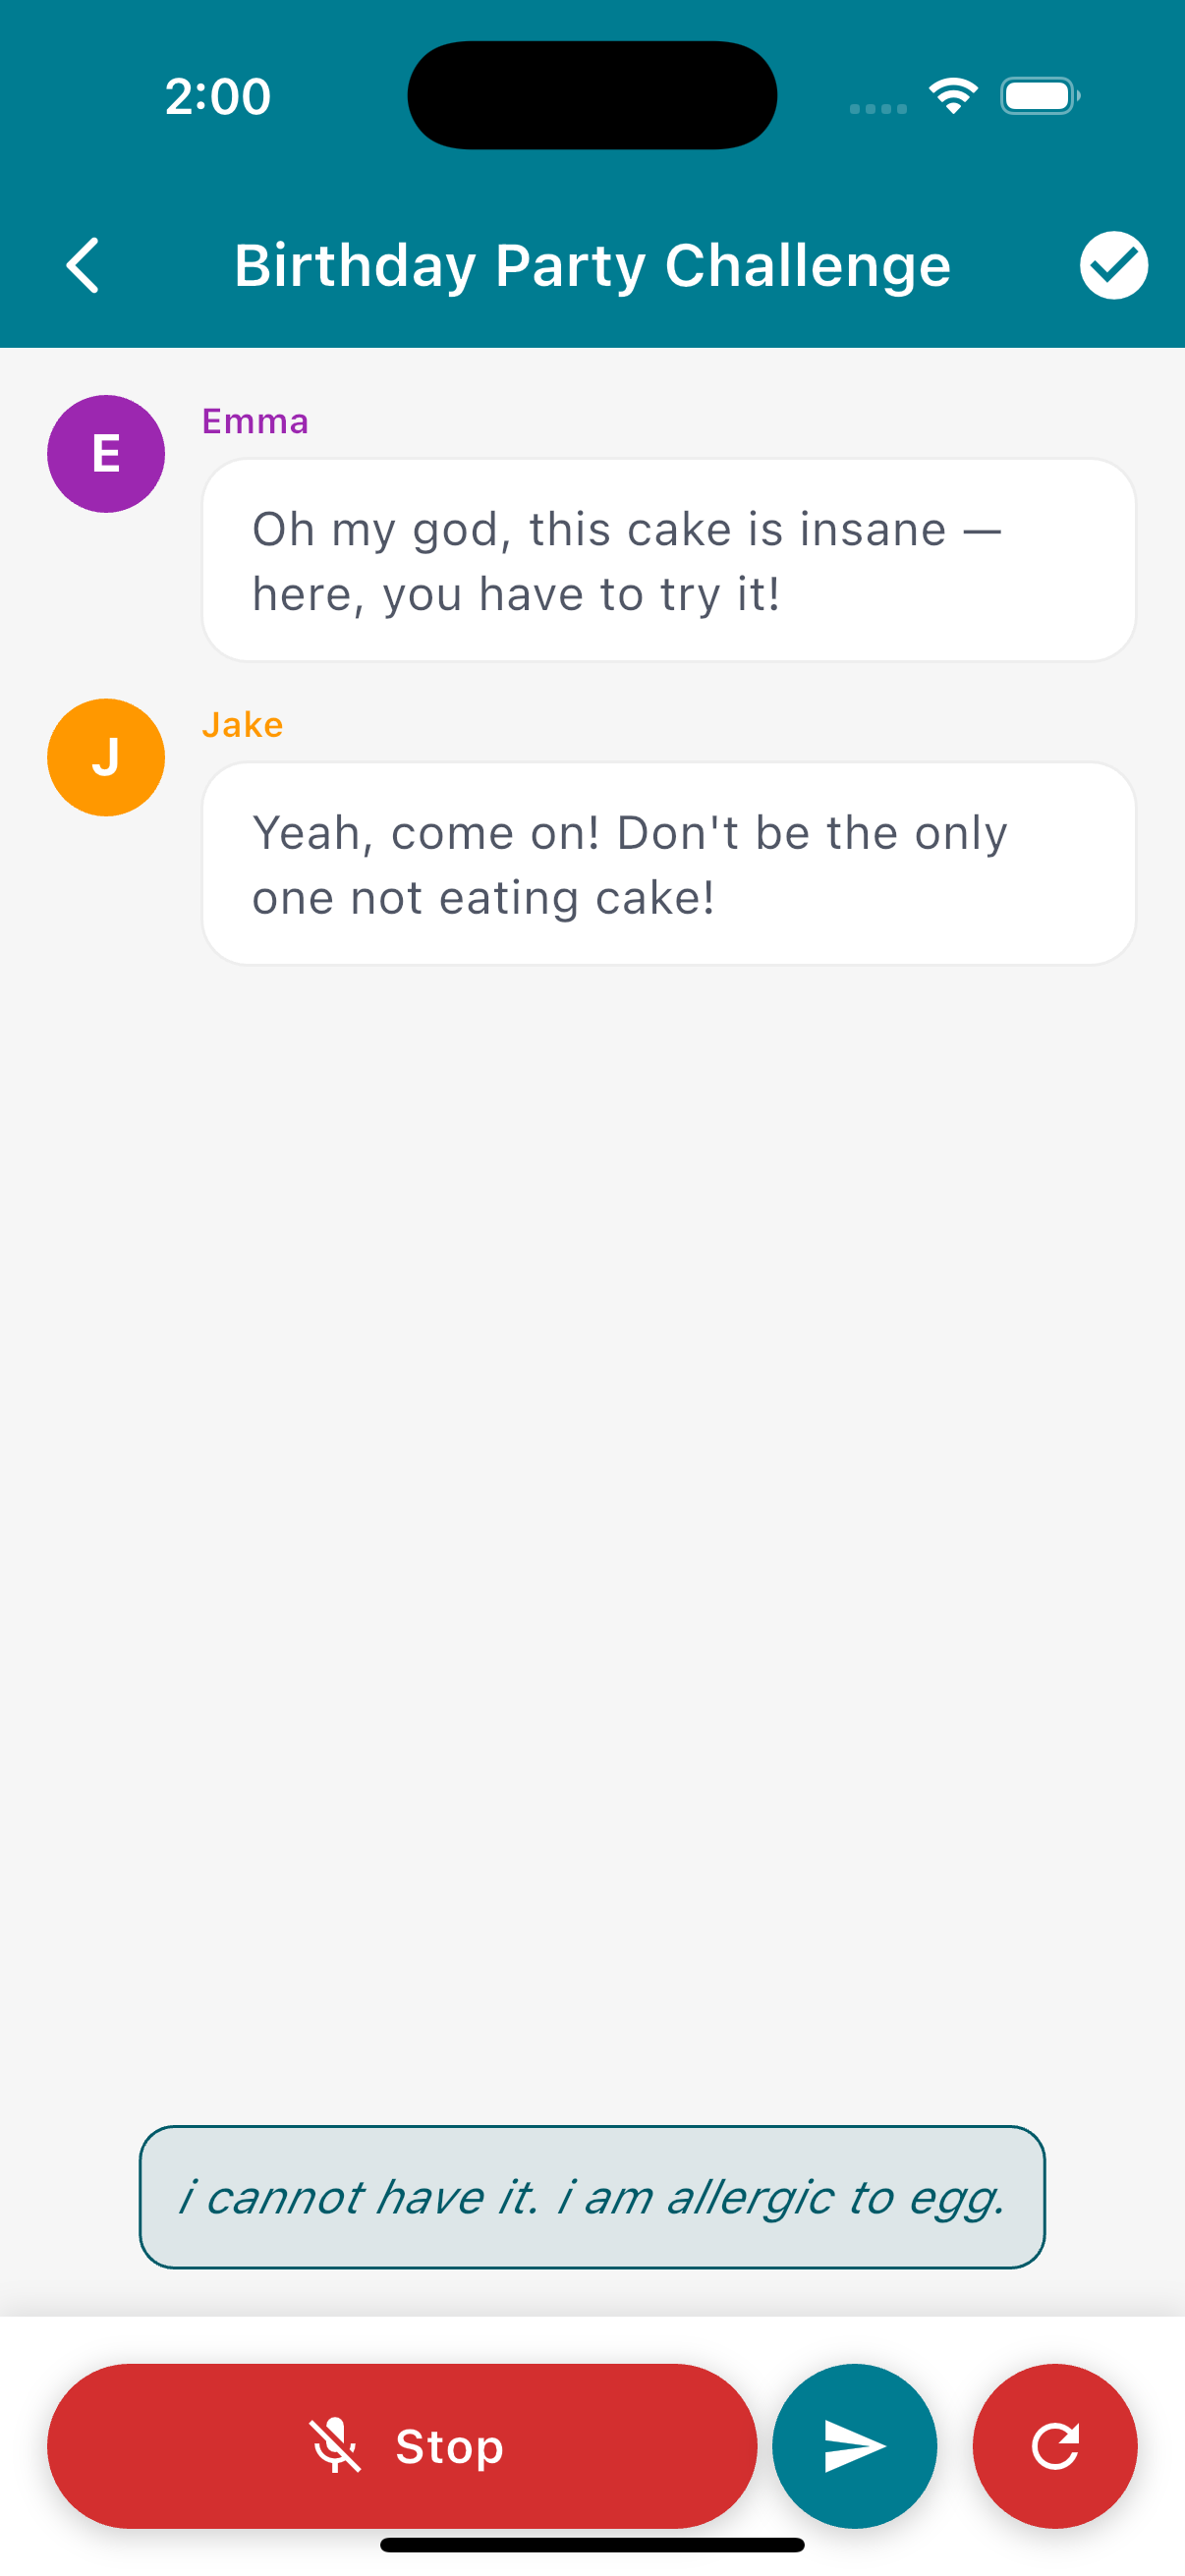
\includegraphics[width=0.8\textwidth,height=0.45\textheight,keepaspectratio]{Figures/group_training_user_speech.png}
    \end{minipage}
    \caption{Group Scenario Training Screens}
    \label{fig:group_training}
\end{figure}

In regard to reinforcing the distinct voice elements and individual traits of the characters, voice distinctiveness and character individualization is kept consistent throughout the entire training session. This enhances the immersive training experience, allowing for the practice of self-advocacy skills in situational role-play interactions. These scenarios are designed to be vividly memorable, comprising significant portions of the user's training journeys.  

During practice sessions, the voice emotions are monitored for real-time analysis of the user's emotions and stress levels. This real-time assessment ensures appropriate support is given during the sessions. This form of emotional intelligence aids training by keeping the process supportive and confidence-boosting for the duration of the training.


\subsection{Failure Case Management and Recovery}

The AI training exercise incorporates thorough failure case handling within various system components to create robust training workflows even under system malfunctions. The system addresses three primary failure categories: issues with network connection, speech recognition system issues, and failures during AI replies generation.

\textbf{Speech Recognition Error Handling:} The speech recognition system has sophisticated error handling processes for automatic detection and correction of a number of simple speech recognition errors. For Timeout or Pause errors (or errors containing "timeout", "pause", "no\_match"), the system will attempt a, restart after a 500-millisecond pause. For errors of longer duration, the speech recognition system will display error feedback of "no speech detected" for no-match, "Speech recognition is listening" for timeout, "microphone detection error" for audio issues, "network error" for connectivity problems, and "microphone permission required" for permission restrictions.

\textbf{AI Response Failure Recovery:} When OpenAI API calls fail due to network issues or service unavailability, the system employs contextual fallback response generation. For individual restaurant scenarios, fallback responses are generated based on conversation context and user allergy profiles, ensuring training continuity even without API connectivity. The system includes response validation that detects unusable AI outputs (empty responses, error messages, malformed JSON, or responses shorter than 10 characters) and automatically generates contextual alternatives using local conversation analysis.

\textbf{Multi-Character Scenario Fallbacks:} Group scenarios implement character-specific fallback responses that maintain training effectiveness when AI services fail. The system provides stage-appropriate fallback responses where early conversation stages (1-2) maintain dismissive peer pressure patterns ("Come on, just try it" or "Don't be difficult"), questioning stages (3) include concern expressions ("Wait, what actually happens if you eat it?"), and supportive stages (4+) offer empathetic responses ("Oh my god, I'm so sorry! I had no idea it was that serious"). Each character maintains consistent personality traits through predefined fallback response pools that ensure realistic peer interaction even during technical failures.

\textbf{Text-to-Speech Failure Management:} The TTS system automatically switches from OpenAI neural voices to device-native TTS in case of OpenAI service unavailability, network issues, or API failures. The fallback system preserves conversational continuity with timed callback animation management to ensure character TTS device animation slipstream, where device TTS is used in sync with character TTS. TTS request timeouts of 20 seconds prevent indefinite waiting and allow for automatic fallback activation during service unavailability.

\textbf{Conversation Recovery and Assessment:} When training sessions are interrupted by technical failures, the system provides fallback assessment generation that evaluates partial conversations. The fallback assessment awards points for completed actions (8 points for allergy disclosure if achieved, 6 points for basic clarity) while providing constructive feedback about incomplete sessions: "This conversation was ended early. Keep practicing to improve your allergy communication skills!" The system maintains conversation context across failure recovery, enabling session resumption where possible and ensuring users can continue training despite technical interruptions.

These comprehensive failure handling mechanisms ensure that technical issues do not compromise the educational value of training sessions, maintaining user confidence and learning momentum even when system components experience difficulties.


\subsection{Feedback System Implementation}

The application implements distinct feedback mechanisms tailored for individual restaurant scenarios and multi-character group scenarios, each designed to address specific learning objectives and assessment criteria appropriate to their respective training contexts.

\textbf{AI-Powered Conversation Analysis:} For individual restaurant scenarios, the system employs sophisticated natural language processing to analyze each conversation turn through the Assessment Engine. The technical implementation uses pattern matching algorithms that scan user input for specific behavioral indicators including allergy mention detection (checking for user's specific allergens and keywords like "allergic to", "allergy", "can't eat"), question asking identification (detecting question marks and interrogative words like "what", "how", "does it contain", "is there"), clarity assessment (evaluating sentence completion, specific language usage, and grammar indicators with scores from 0-10), and proactiveness scoring (awarding higher points for early allergy disclosure and initiative-taking behaviors).

The scoring system implements a comprehensive point allocation across multiple categories: Core Communication Skills (40 points maximum) covering allergy disclosure (0-15 points based on frequency of mentions), clarity (0-10 points from average turn clarity), and proactiveness (0-15 points for question-asking frequency); Safety Awareness (30 points maximum) including ingredient inquiry assessment (detecting keywords like "ingredient", "contain", "what's in", "made with") and risk assessment evaluation; and Social Skills (20 points maximum) measuring confidence and politeness through conversation length analysis and polite language detection ("please", "thank", "excuse me").

\textbf{Difficulty-Adaptive Scoring:} Advanced scenarios employ enhanced scoring criteria including cross-contamination awareness (20 points for detecting keywords like "cross", "contamination", "shared", "fryer", "equipment"), preparation method inquiries (15 points for asking about cooking processes), and unsafe food ordering penalties (-30 points with partial credit for corrections). The system uses menu-specific food analysis to determine safety by matching ordered items against user allergy profiles, with specific dish recognition for items like chocolate brownie (contains milk and eggs) and satay chicken (contains peanuts).

\begin{figure}[htbp]
    \centering
    \begin{minipage}[b]{0.45\textwidth}
        \centering
        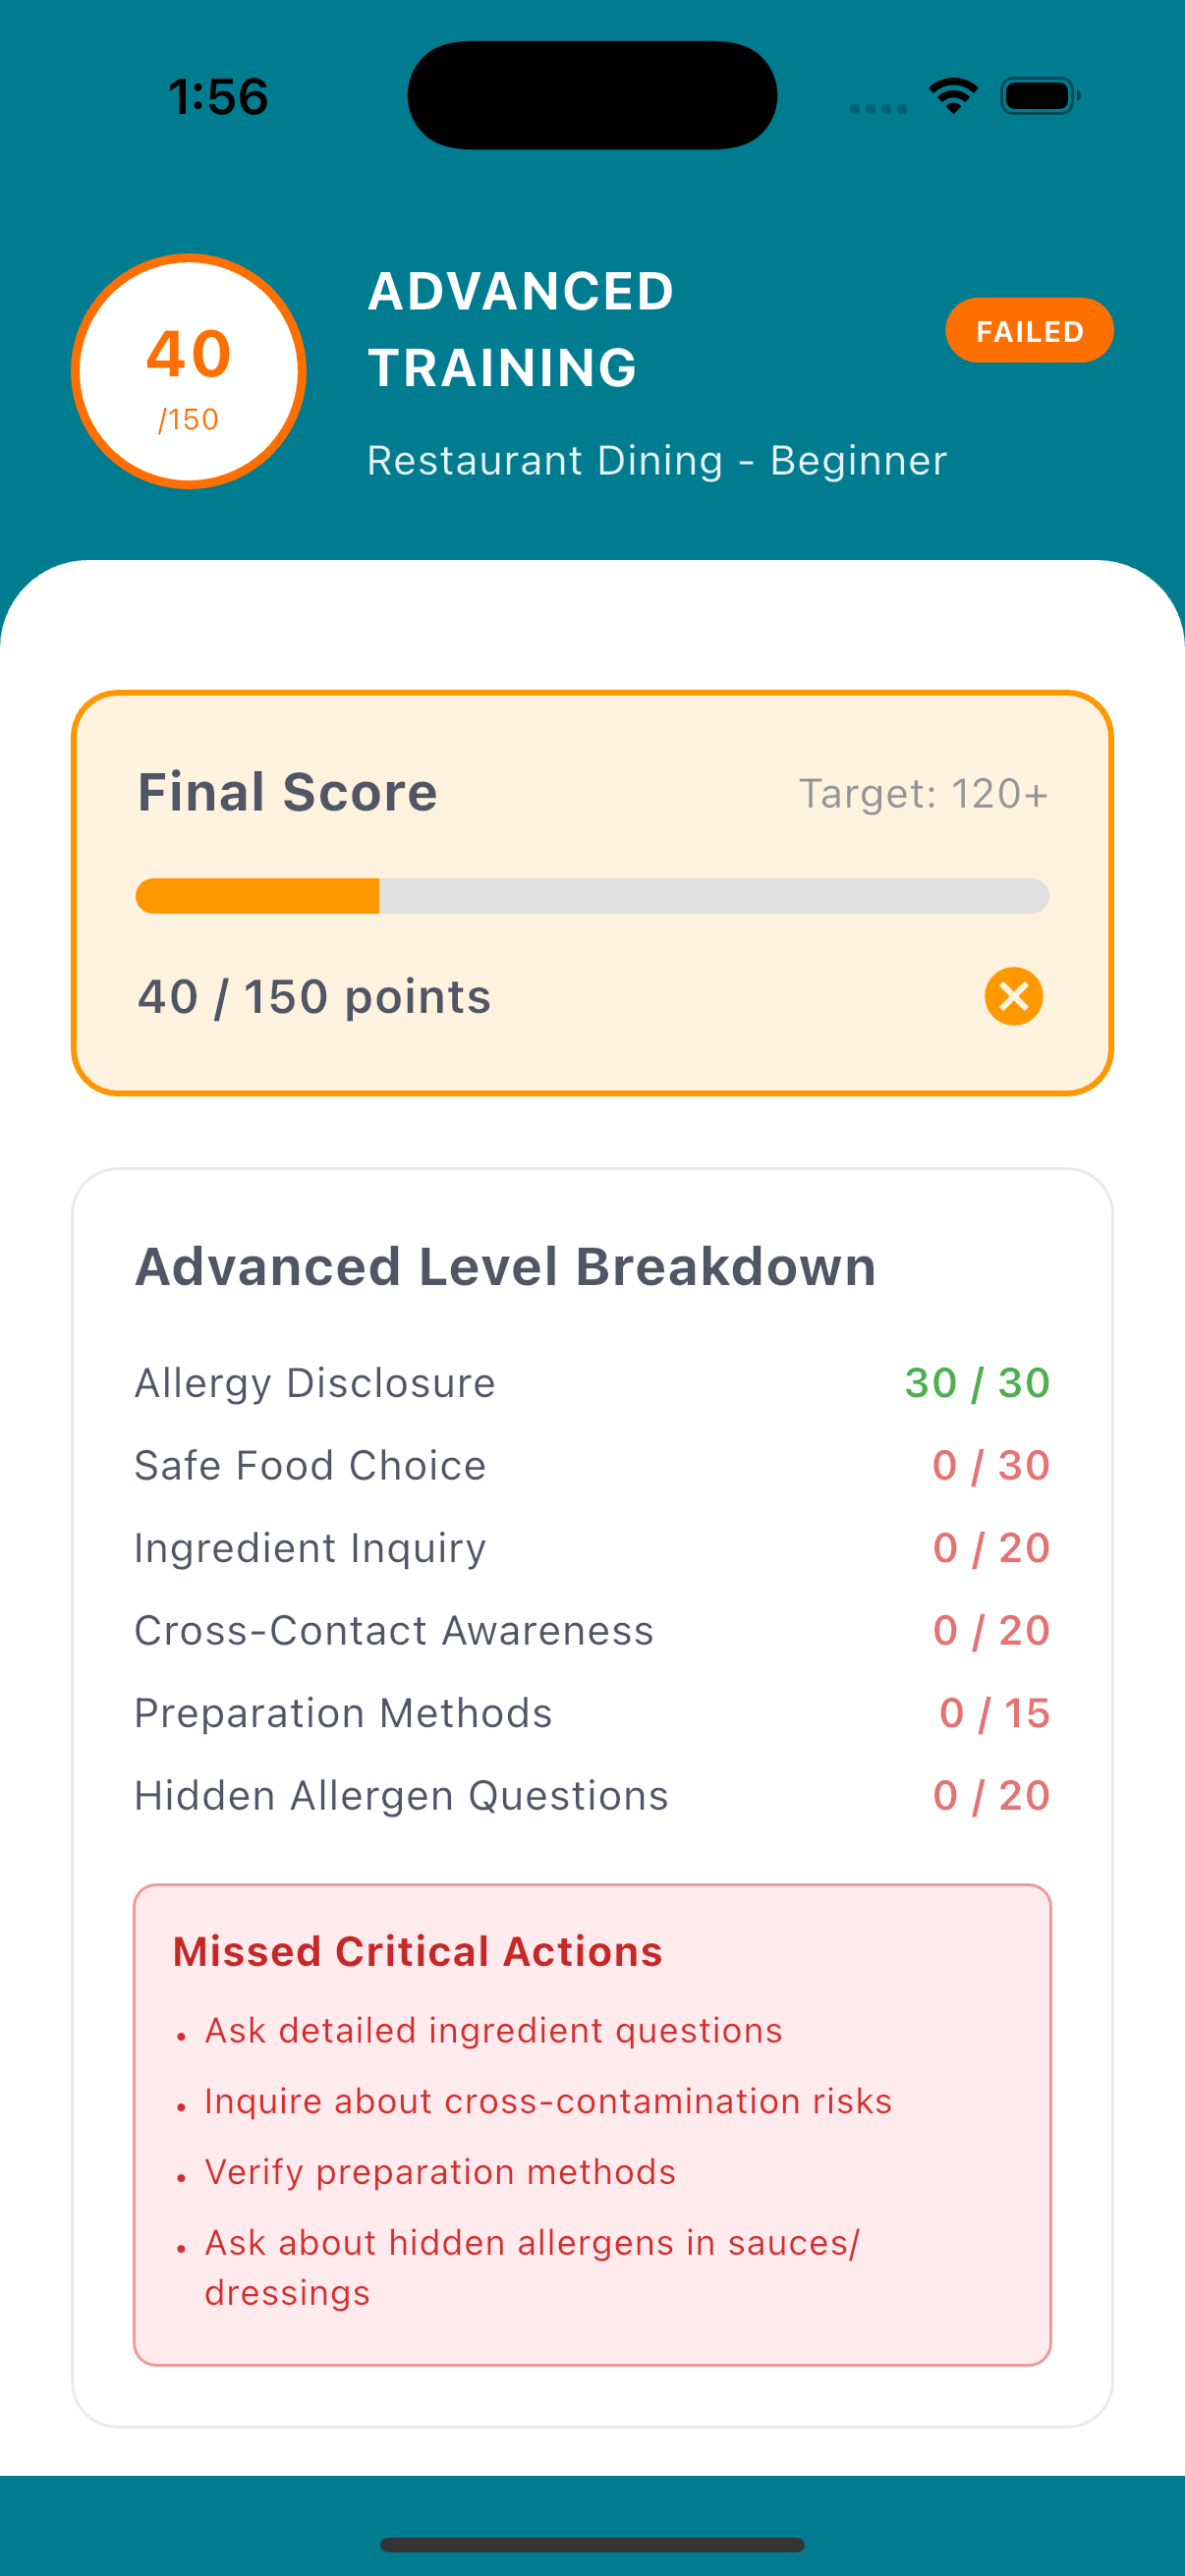
\includegraphics[width=0.8\textwidth,height=0.45\textheight,keepaspectratio]{Figures/resto_feedback_screen.png}
    \end{minipage}
    \hfill
    \begin{minipage}[b]{0.45\textwidth}
        \centering
        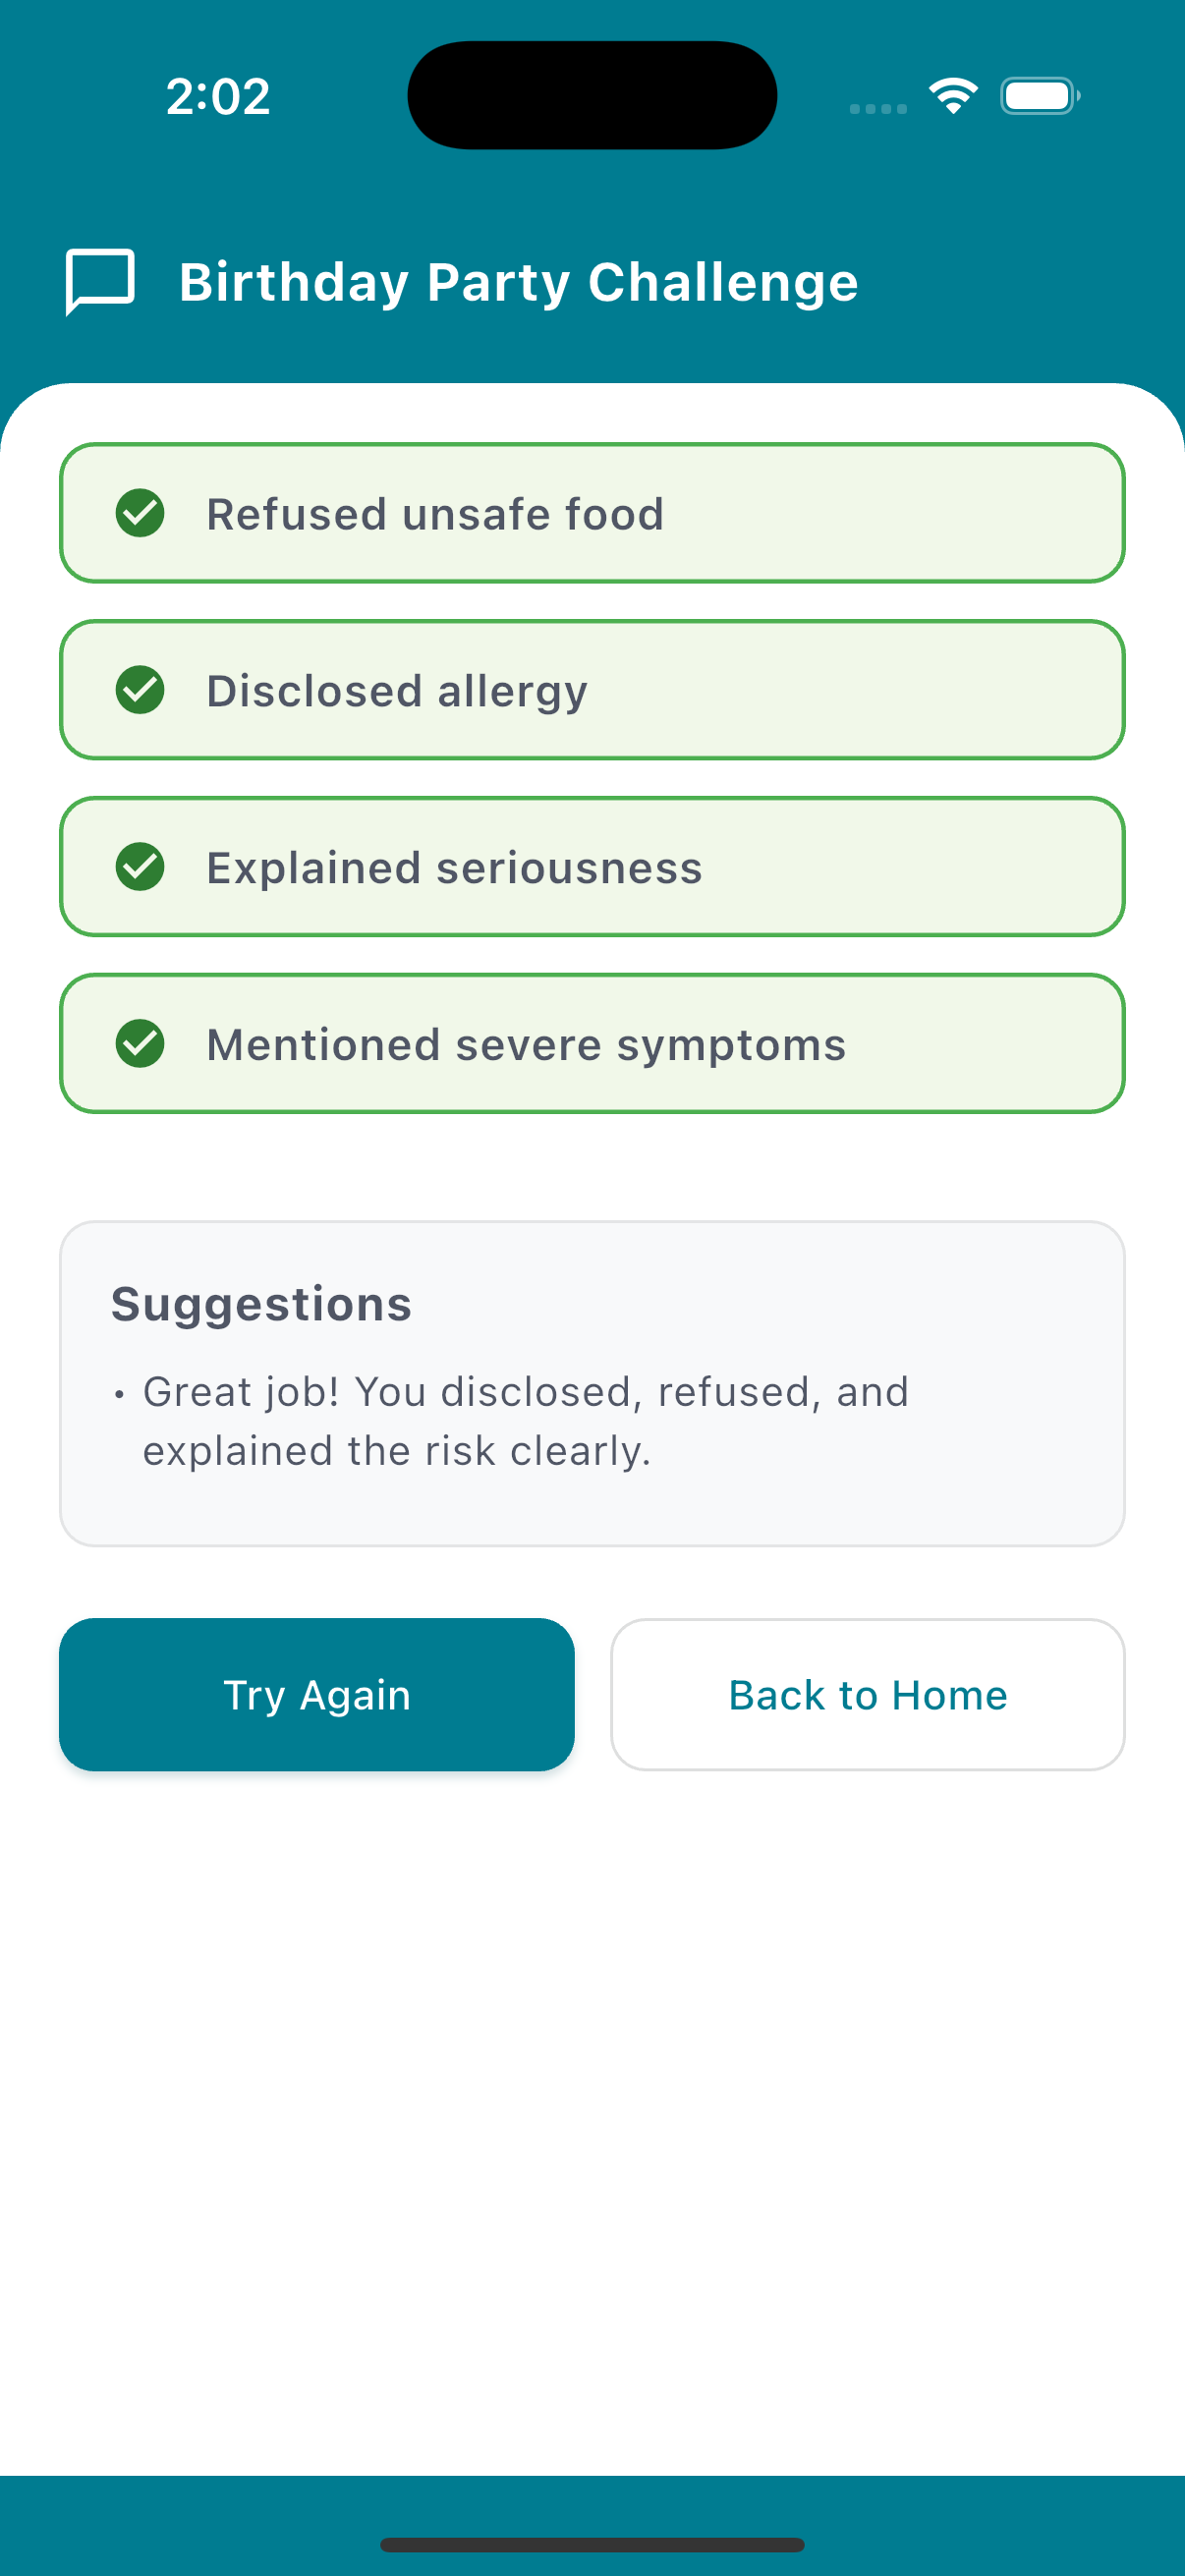
\includegraphics[width=0.8\textwidth,height=0.45\textheight,keepaspectratio]{Figures/group_training_feedback_screen.png}
    \end{minipage}
     \caption{Feedback Screens for Group and Restaurant Scenarios}
     \label{fig:feedback-screen-screenshots}
    
\end{figure}

For group scenarios, the feedback system utilizes a simplified boolean outcome tracking through the GroupTrainingOutcome model, monitoring four critical self-advocacy behaviors: allergy mention, unsafe food refusal, severity explanation, and severe symptom disclosure. The GroupFeedbackScreen displays these outcomes through color-coded indicators with green checkmarks for completed actions and orange warning icons for missed opportunities. The feedback includes specific actionable suggestions such as "Practice a clear refusal like: 'No thanks, I can't eat that'" for users who failed to refuse unsafe food, or "Mention outcomes: 'I could have trouble breathing/anaphylaxis'" for those who didn't communicate severity. This binary success tracking approach reflects the peer pressure scenario's focus on essential safety communication rather than nuanced service interaction skills.


\section{Daily Reminder System}

The reminder system provides a straightforward notification mechanism to promote consistent adrenaline pen carrying through daily check-in prompts. The implementation focuses on simplicity and reliability while maintaining user engagement through randomized timing to prevent habituation.


\begin{figure}[htbp]
    \centering
    \begin{minipage}[b]{0.45\textwidth}
        \centering
        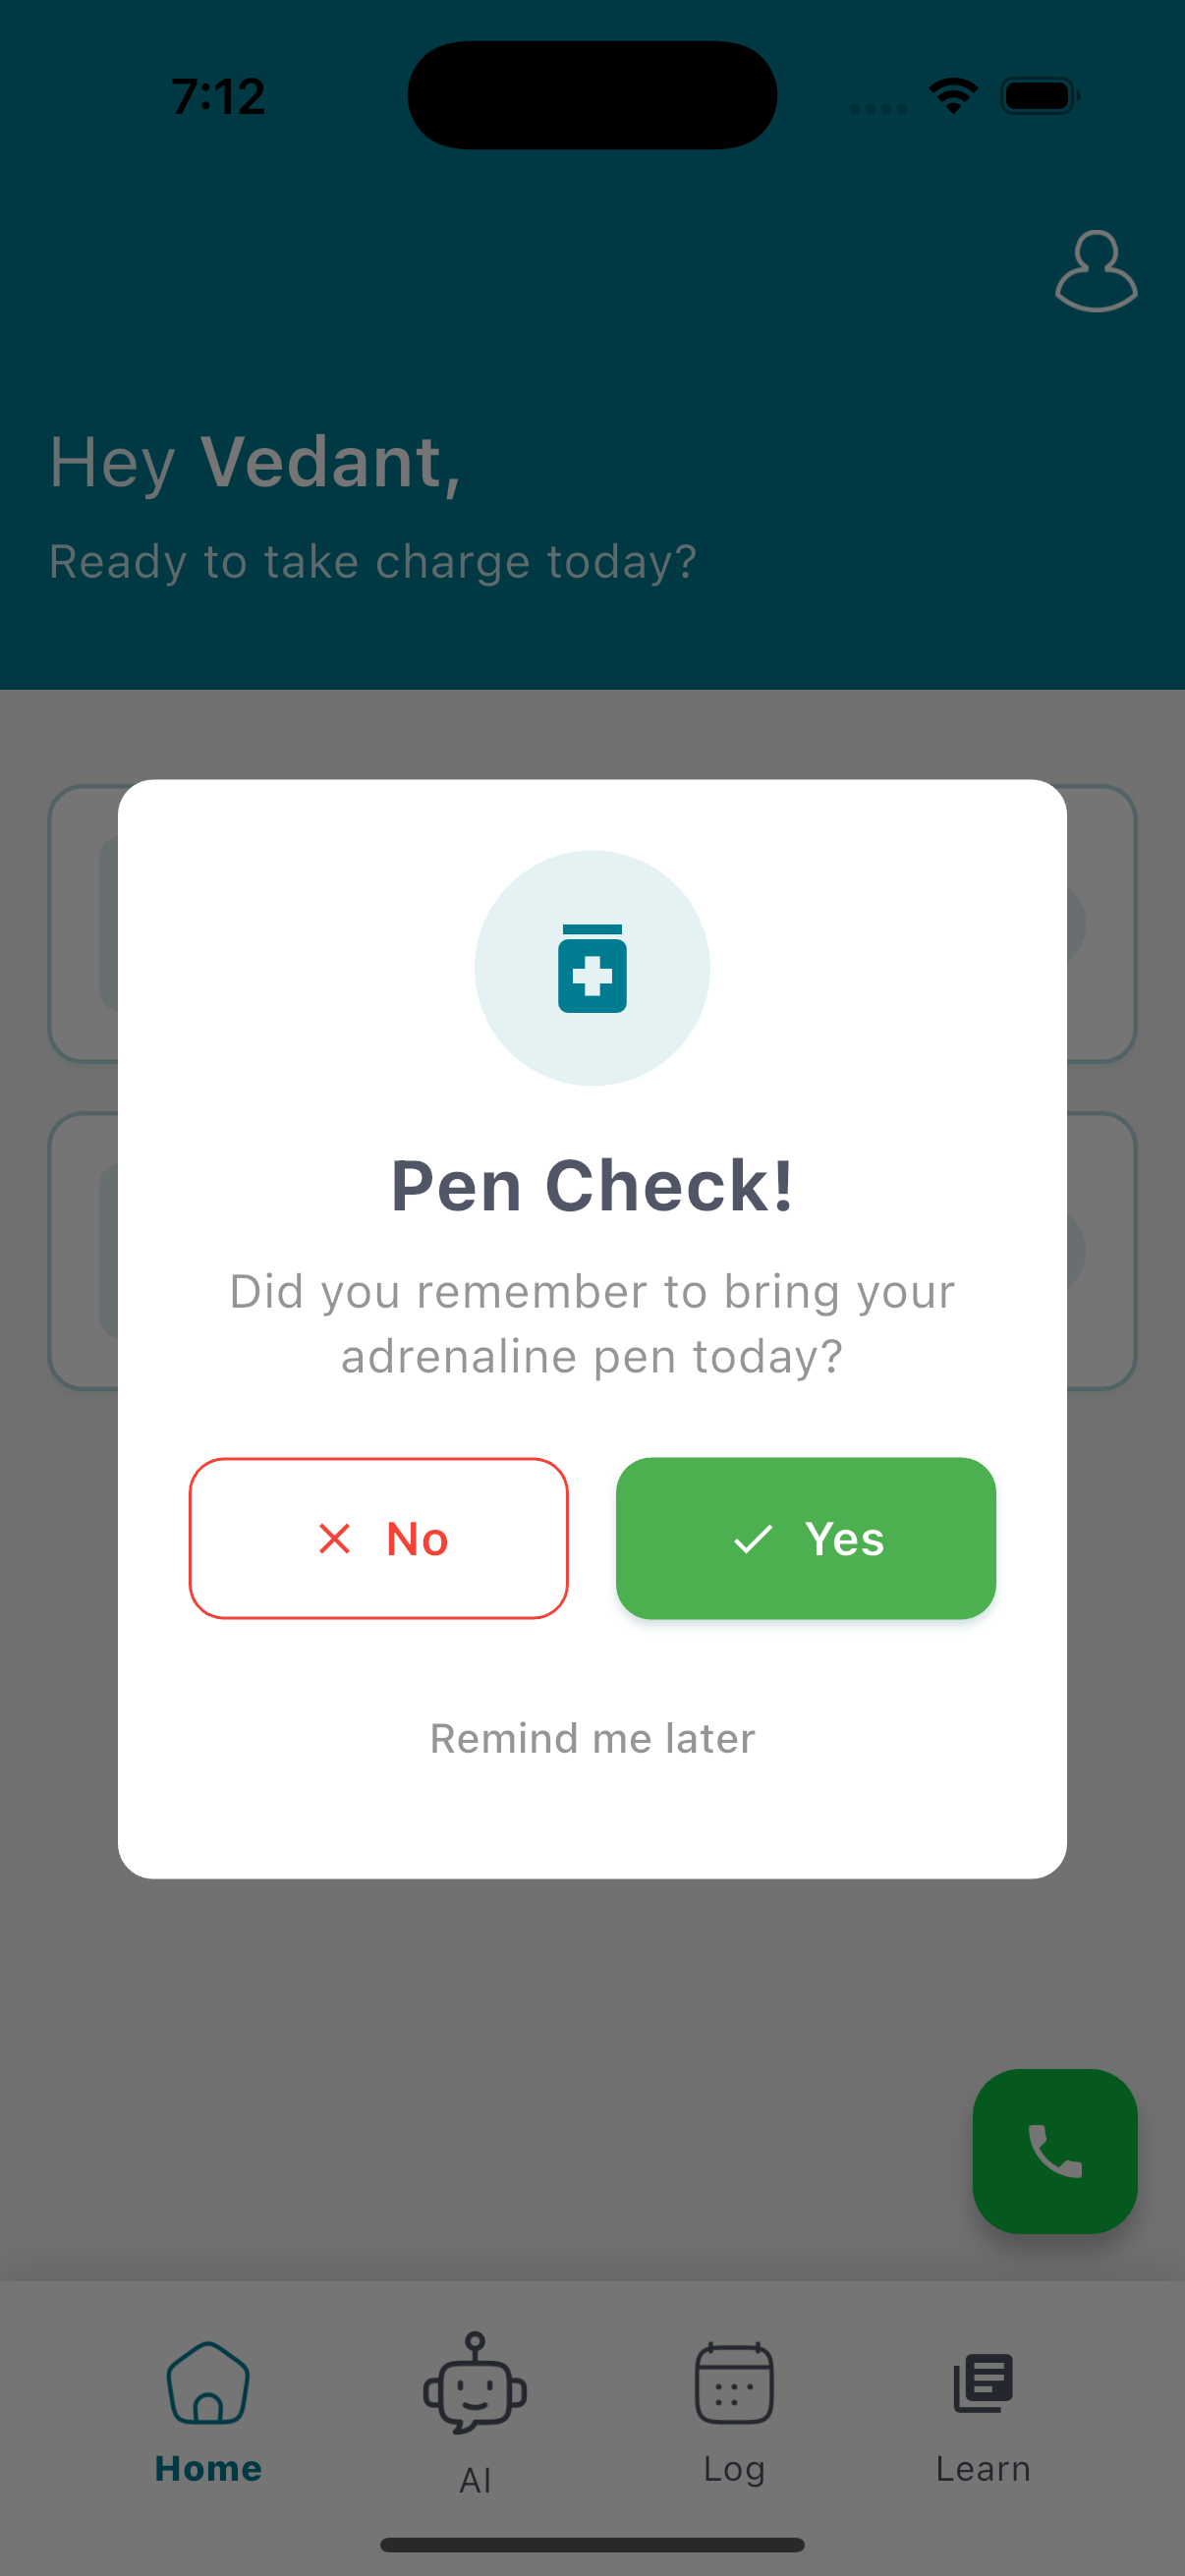
\includegraphics[width=0.8\textwidth,height=0.45\textheight,keepaspectratio]{Figures/pen_reminder_dialogue.png}
     
        \label{fig:pen-reminder-dialog}
    \end{minipage}
    \hfill
    \begin{minipage}[b]{0.45\textwidth}
        \centering
        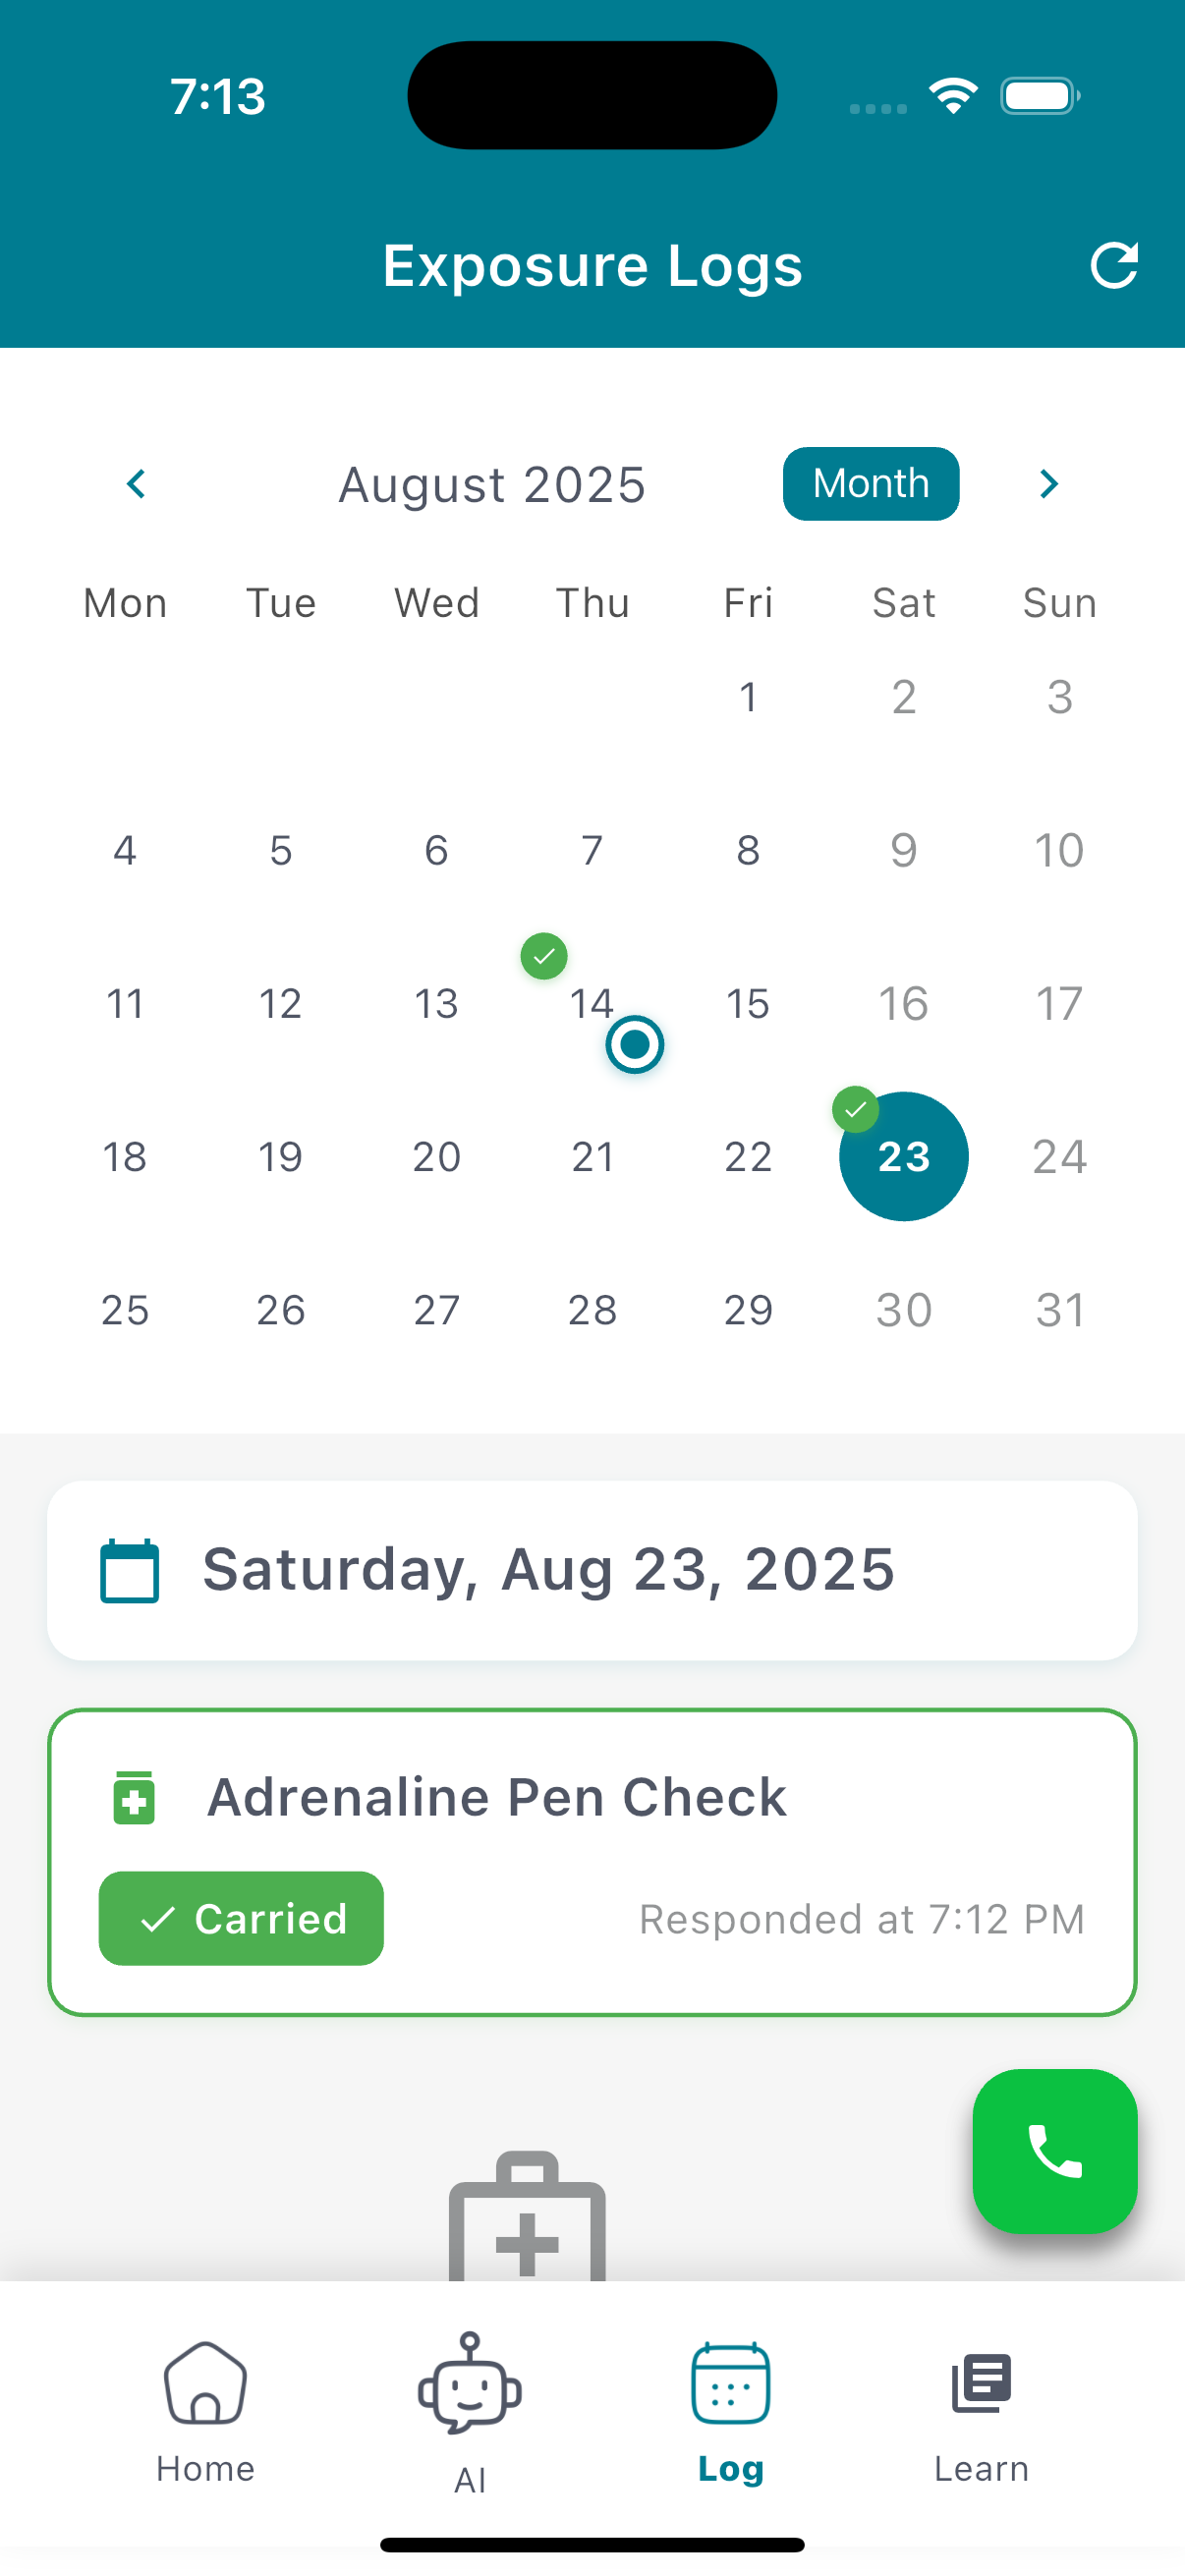
\includegraphics[width=0.8\textwidth,height=0.45\textheight,keepaspectratio]{Figures/pen_reminder_log.png}
      
        \label{fig:pen-reminder-log}
    \end{minipage}
    \caption{Daily Reminder System Interface and Notification Management}
    \label{fig:reminder-system-screenshots}
\end{figure}

\subsection{Implementation and User Interaction}

The core innovation of the reminder system lies in its randomized scheduling approach that generates notification times between 8:00 AM and 6:00 PM each day using standard random number generation for both hour (8-17) and minute (0-59) values. This unpredictability maintains user attention and prevents the psychological habituation that occurs with predictable reminder patterns. Cross-platform scheduling utilizes Flutter's local notifications plugin with timezone support, ensuring reliable delivery across both Android and iOS devices through exact timing scheduling modes that maintain notification accuracy even when the application is not actively running.

The notification interaction model prioritizes simplicity and immediate response capture. When users receive the daily reminder notification titled "Daily Pen Check!" with the message "Quick check-in! Did you remember to bring your adrenaline pen today?", tapping the notification opens a modal dialog within the application. The dialog presents two clear response options: "Yes" (indicating the user has their pen) or "No" (indicating they forgot their pen), along with a "Remind me later" option for users who prefer to respond at a more convenient time. Each response is immediately stored in Firebase Firestore with the current date and boolean pen-carried status, creating a simple compliance tracking record.

The system maintains straightforward response tracking through Firebase Firestore, storing each daily response as a document with date and compliance status. This enables basic pattern recognition where users can review their compliance history through calendar visualization, showing green markers for days when the pen was carried and red markers for missed days. Response data supports fundamental analytics including compliance rate calculation, identification of missed days, and basic trend visualization over time, while respecting user privacy by storing only essential compliance information without behavioral analysis or predictive modeling.

\section{Symptom Logging Module}

The symptom logging system provides a straightforward form-based interface for documenting accidental exposures and tracking symptoms. The implementation focuses on capturing essential information about allergic reactions while maintaining simplicity for adolescent users during potentially stressful situations.



\begin{figure}[htbp]
    \centering
    \begin{minipage}[b]{0.3\textwidth}
        \centering
        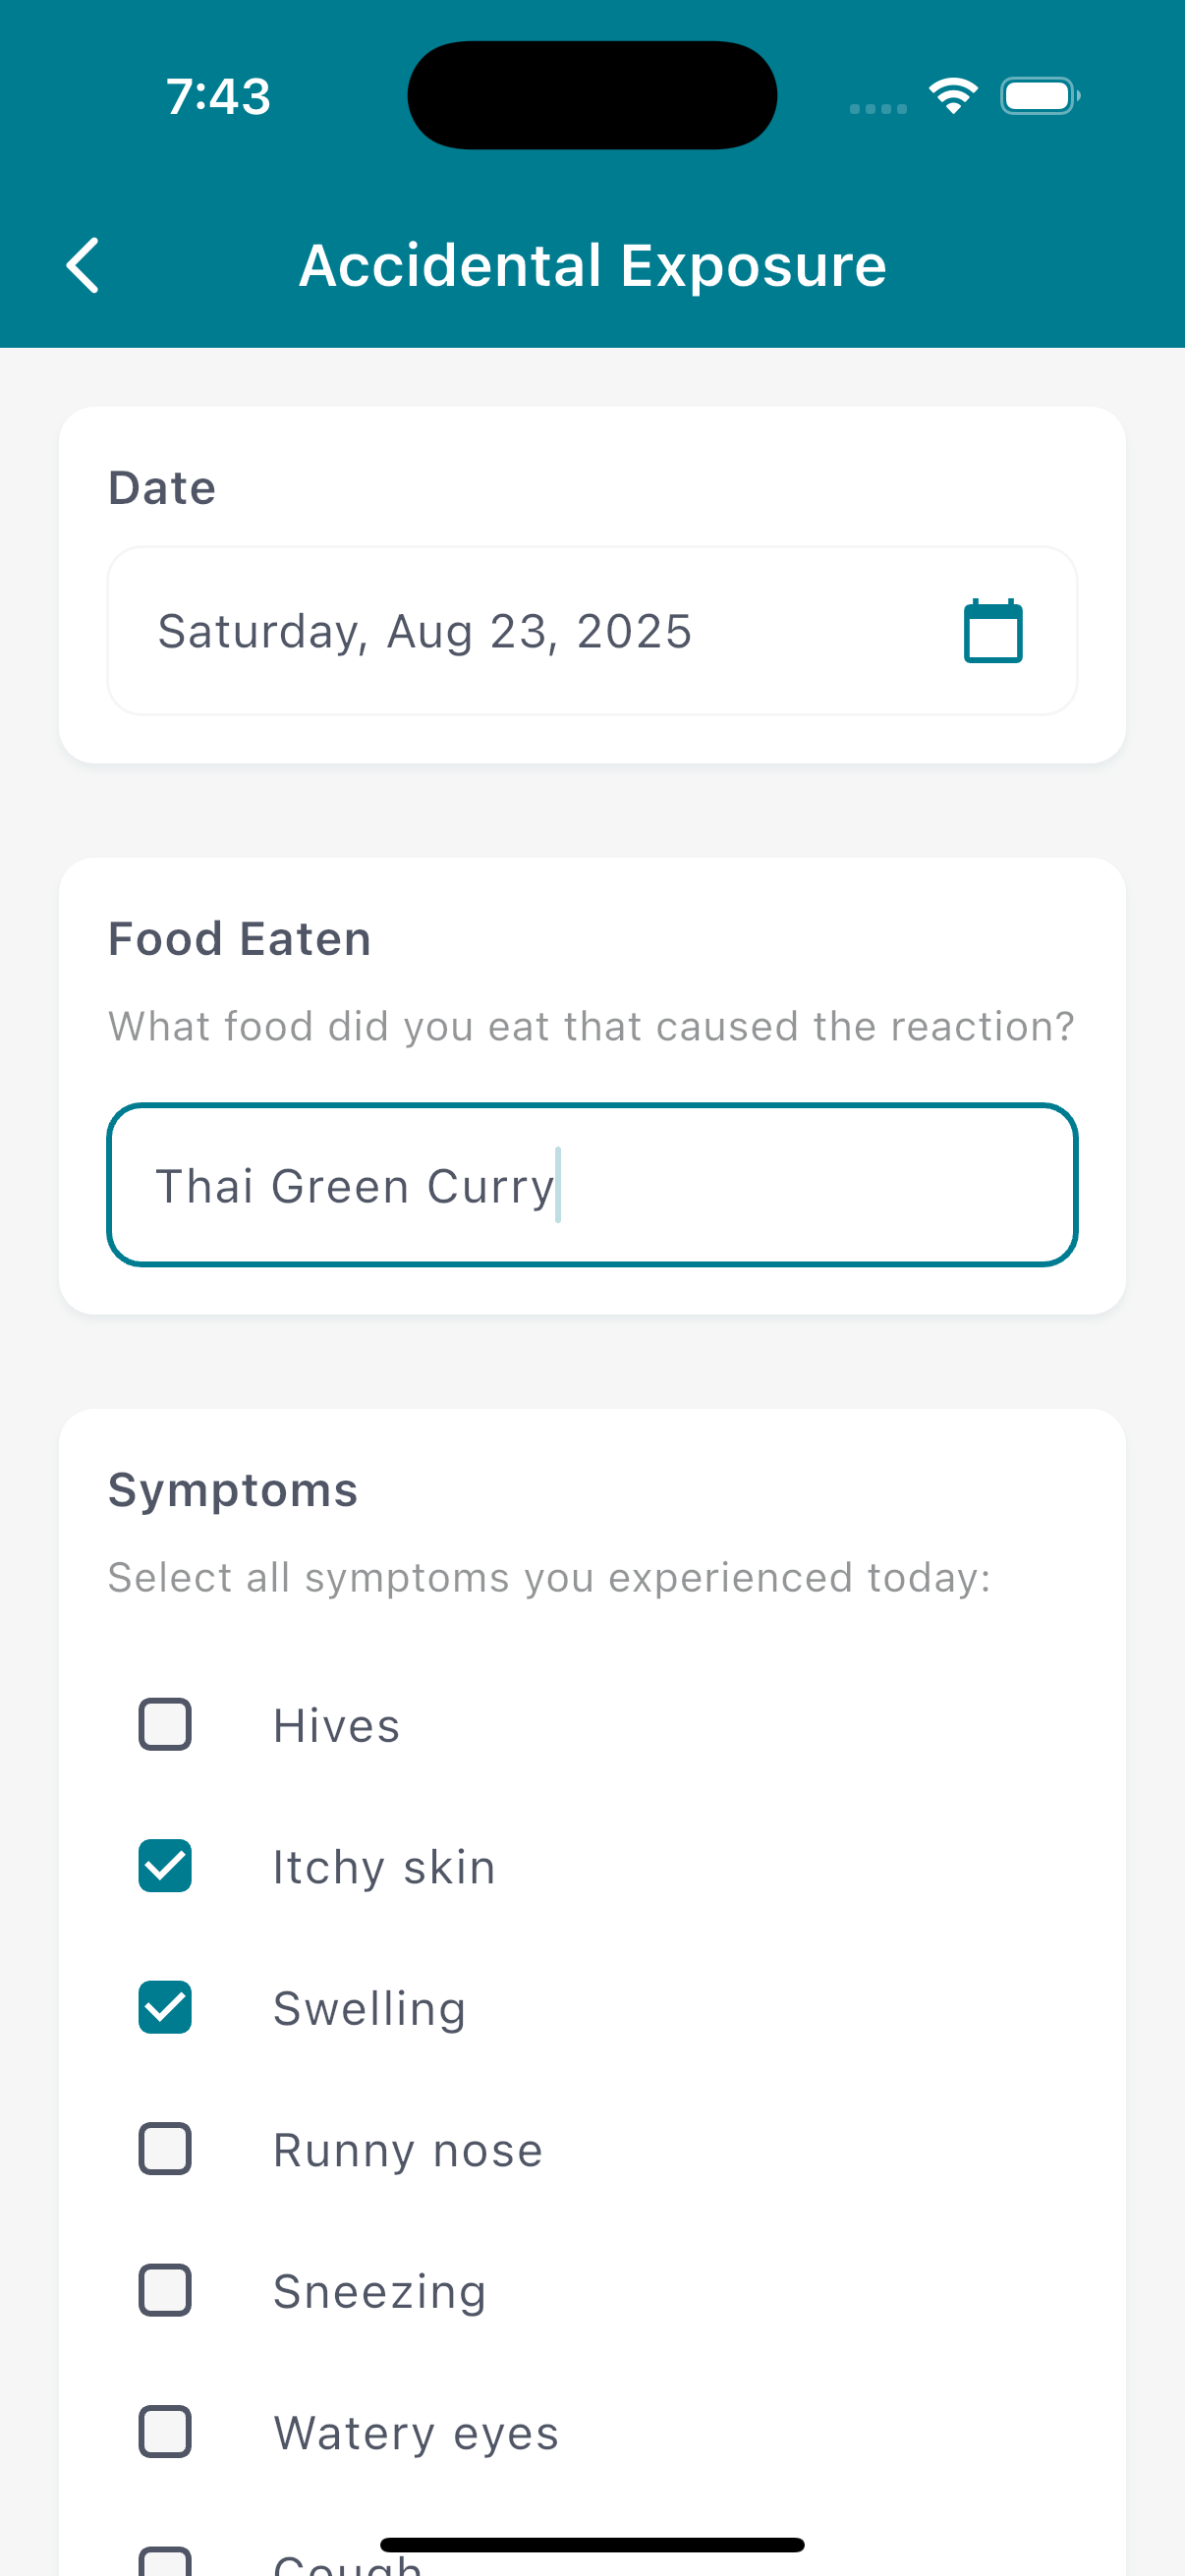
\includegraphics[width=0.9\textwidth,height=0.4\textheight,keepaspectratio]{Figures/symptom_log_1.png}
    \end{minipage}
    \hfill
    \begin{minipage}[b]{0.3\textwidth}
        \centering
        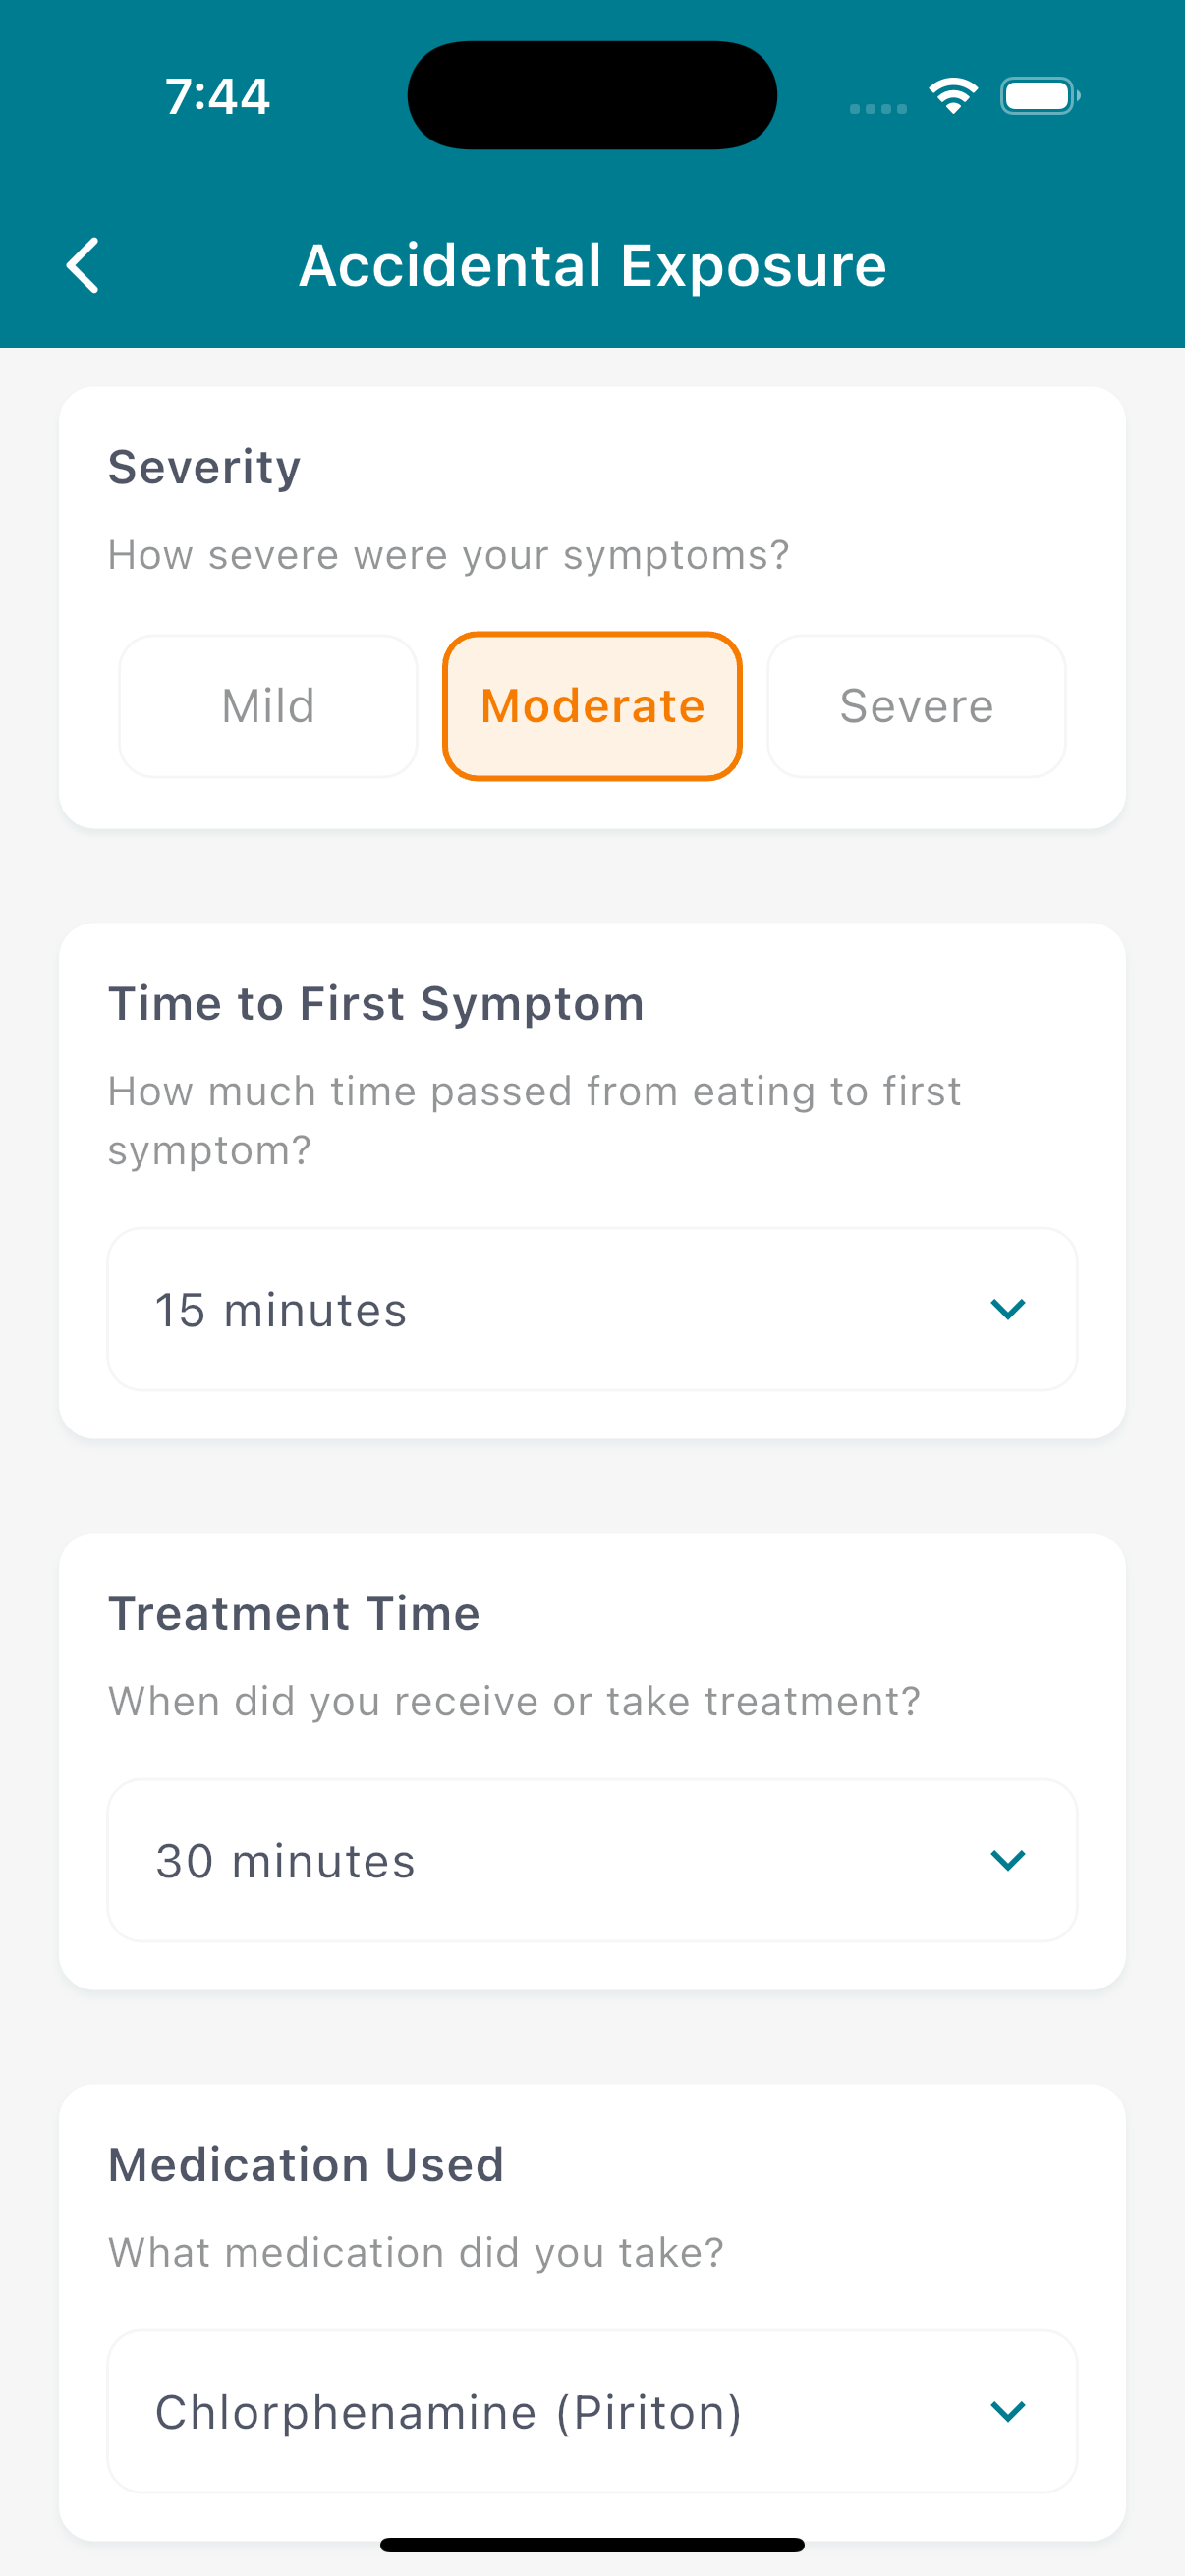
\includegraphics[width=0.9\textwidth,height=0.4\textheight,keepaspectratio]{Figures/symptom_log_2.png}
    \end{minipage}
    \hfill
    \begin{minipage}[b]{0.3\textwidth}
        \centering
        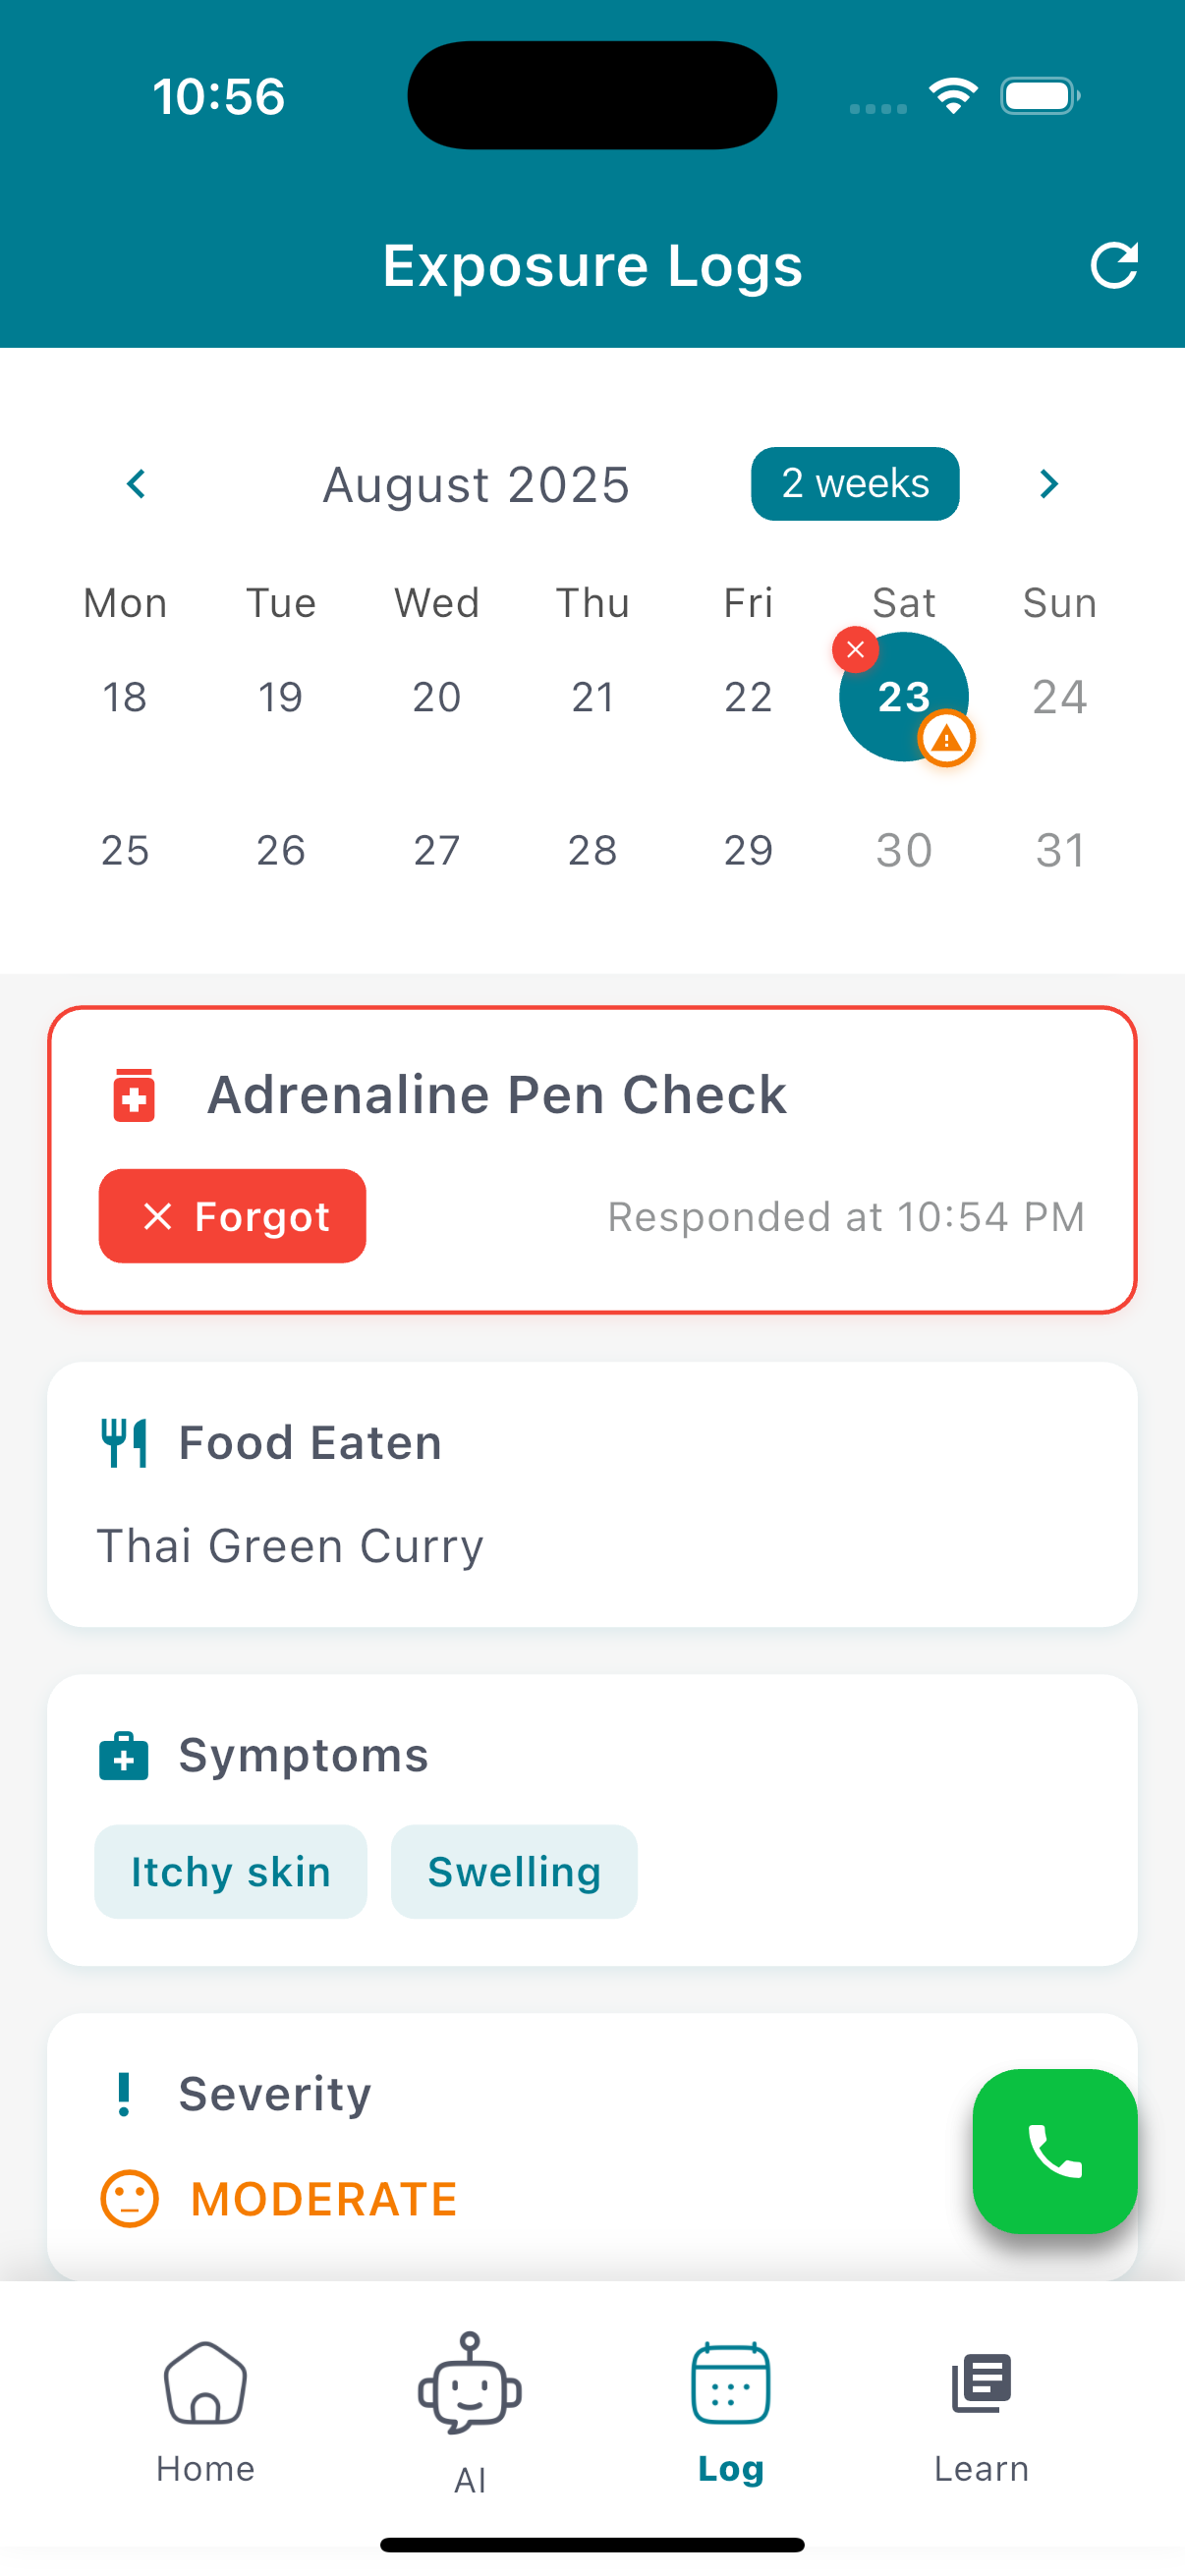
\includegraphics[width=0.9\textwidth,height=0.4\textheight,keepaspectratio]{Figures/symptom_log.png}
    \end{minipage}
    \caption{Symptom Logging Interface with Calendar Integration}
    \label{fig:symptom_log_with_calendar}
\end{figure}

\subsection{Form-Based Data Capture and Calendar Visualization}

The logging interface captures several critical pieces of information on accidental exposures such as: date selection, selection of symptoms from a list of 20 common allergic reaction symptoms (including mild symptoms such as hives, itchy skin, running nose, and headaches, to more severe shortness of breath, difficulty swallowing, throat tightness, rapid heart rate), and severity assessment on a triage scale of three: mild, moderate, severe. Also included are: food eaten details, and timeline information such as symptom onset and treatment onset, medication tracking with boolean flag and details on the particular medication, and context with notes.

The system also integrates with a calendar system using the table calendar plugin. This allows users to navigate visually through months and see exposure logs with event indicators marking the logged exposures. As users navigate through the months, the calendar will show simple indicators on the dates with symptom logs, which can be accessed or added to. Users can also navigate through dates to view existing logs and enter new ones. The calendar also shows pen reminder response data, which integrates compliance tracking with symptom documentation.

Symptom logs are stored with timestamped dates, an array of symptoms, and an indication of their severity, medication used, and note texts about food, all as key-value pairs in Firebase Firestore. The system allows users to perform simple CRUD (create, read, update, and delete) operations for logs. Automatic date-based sorting and straightforward state management through Riverpod providers streamline operations. A log is created for each day with a unique date-based ID, which allows for easy entry modification and supports in-depth editing of previously logged data.





\section{Barcode Scanner Integration}

The product scanning system provides straightforward barcode detection and allergen identification through mobile camera integration and OpenFoodFacts API connectivity. The implementation prioritizes simplicity and reliability while providing essential safety information for food products.



\begin{figure}[htbp]
    \centering
    \begin{minipage}[b]{0.3\textwidth}
        \centering
        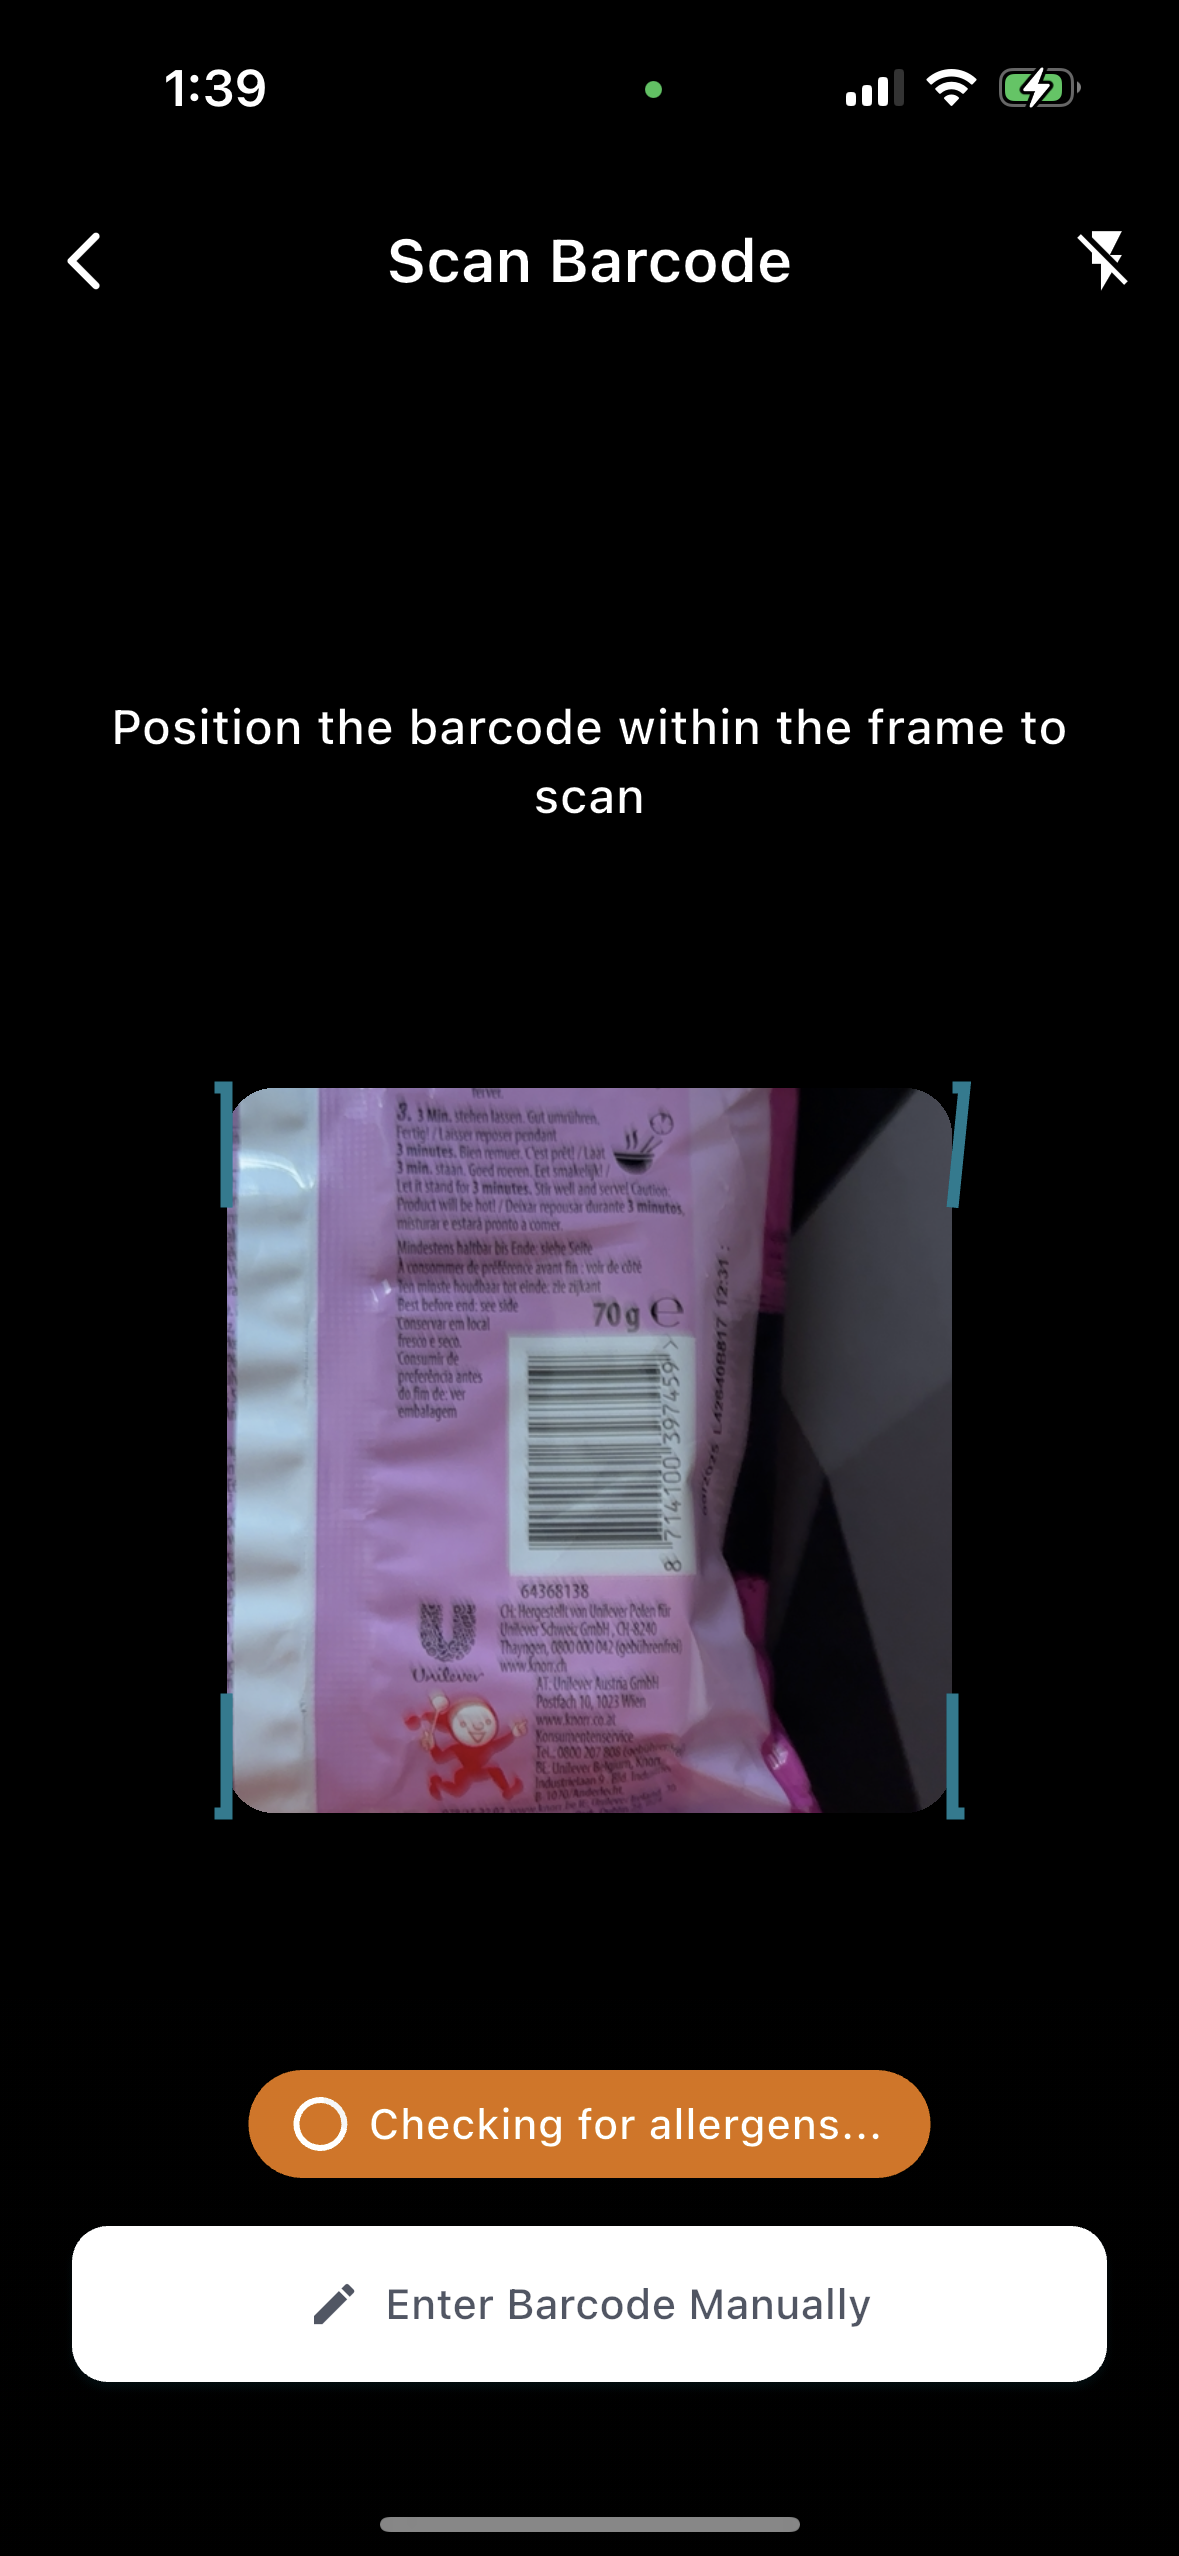
\includegraphics[width=0.9\textwidth,height=0.4\textheight,keepaspectratio]{Figures/barcode_scanner_camera.png}
    \end{minipage}
    \hfill
    \begin{minipage}[b]{0.3\textwidth}
        \centering
        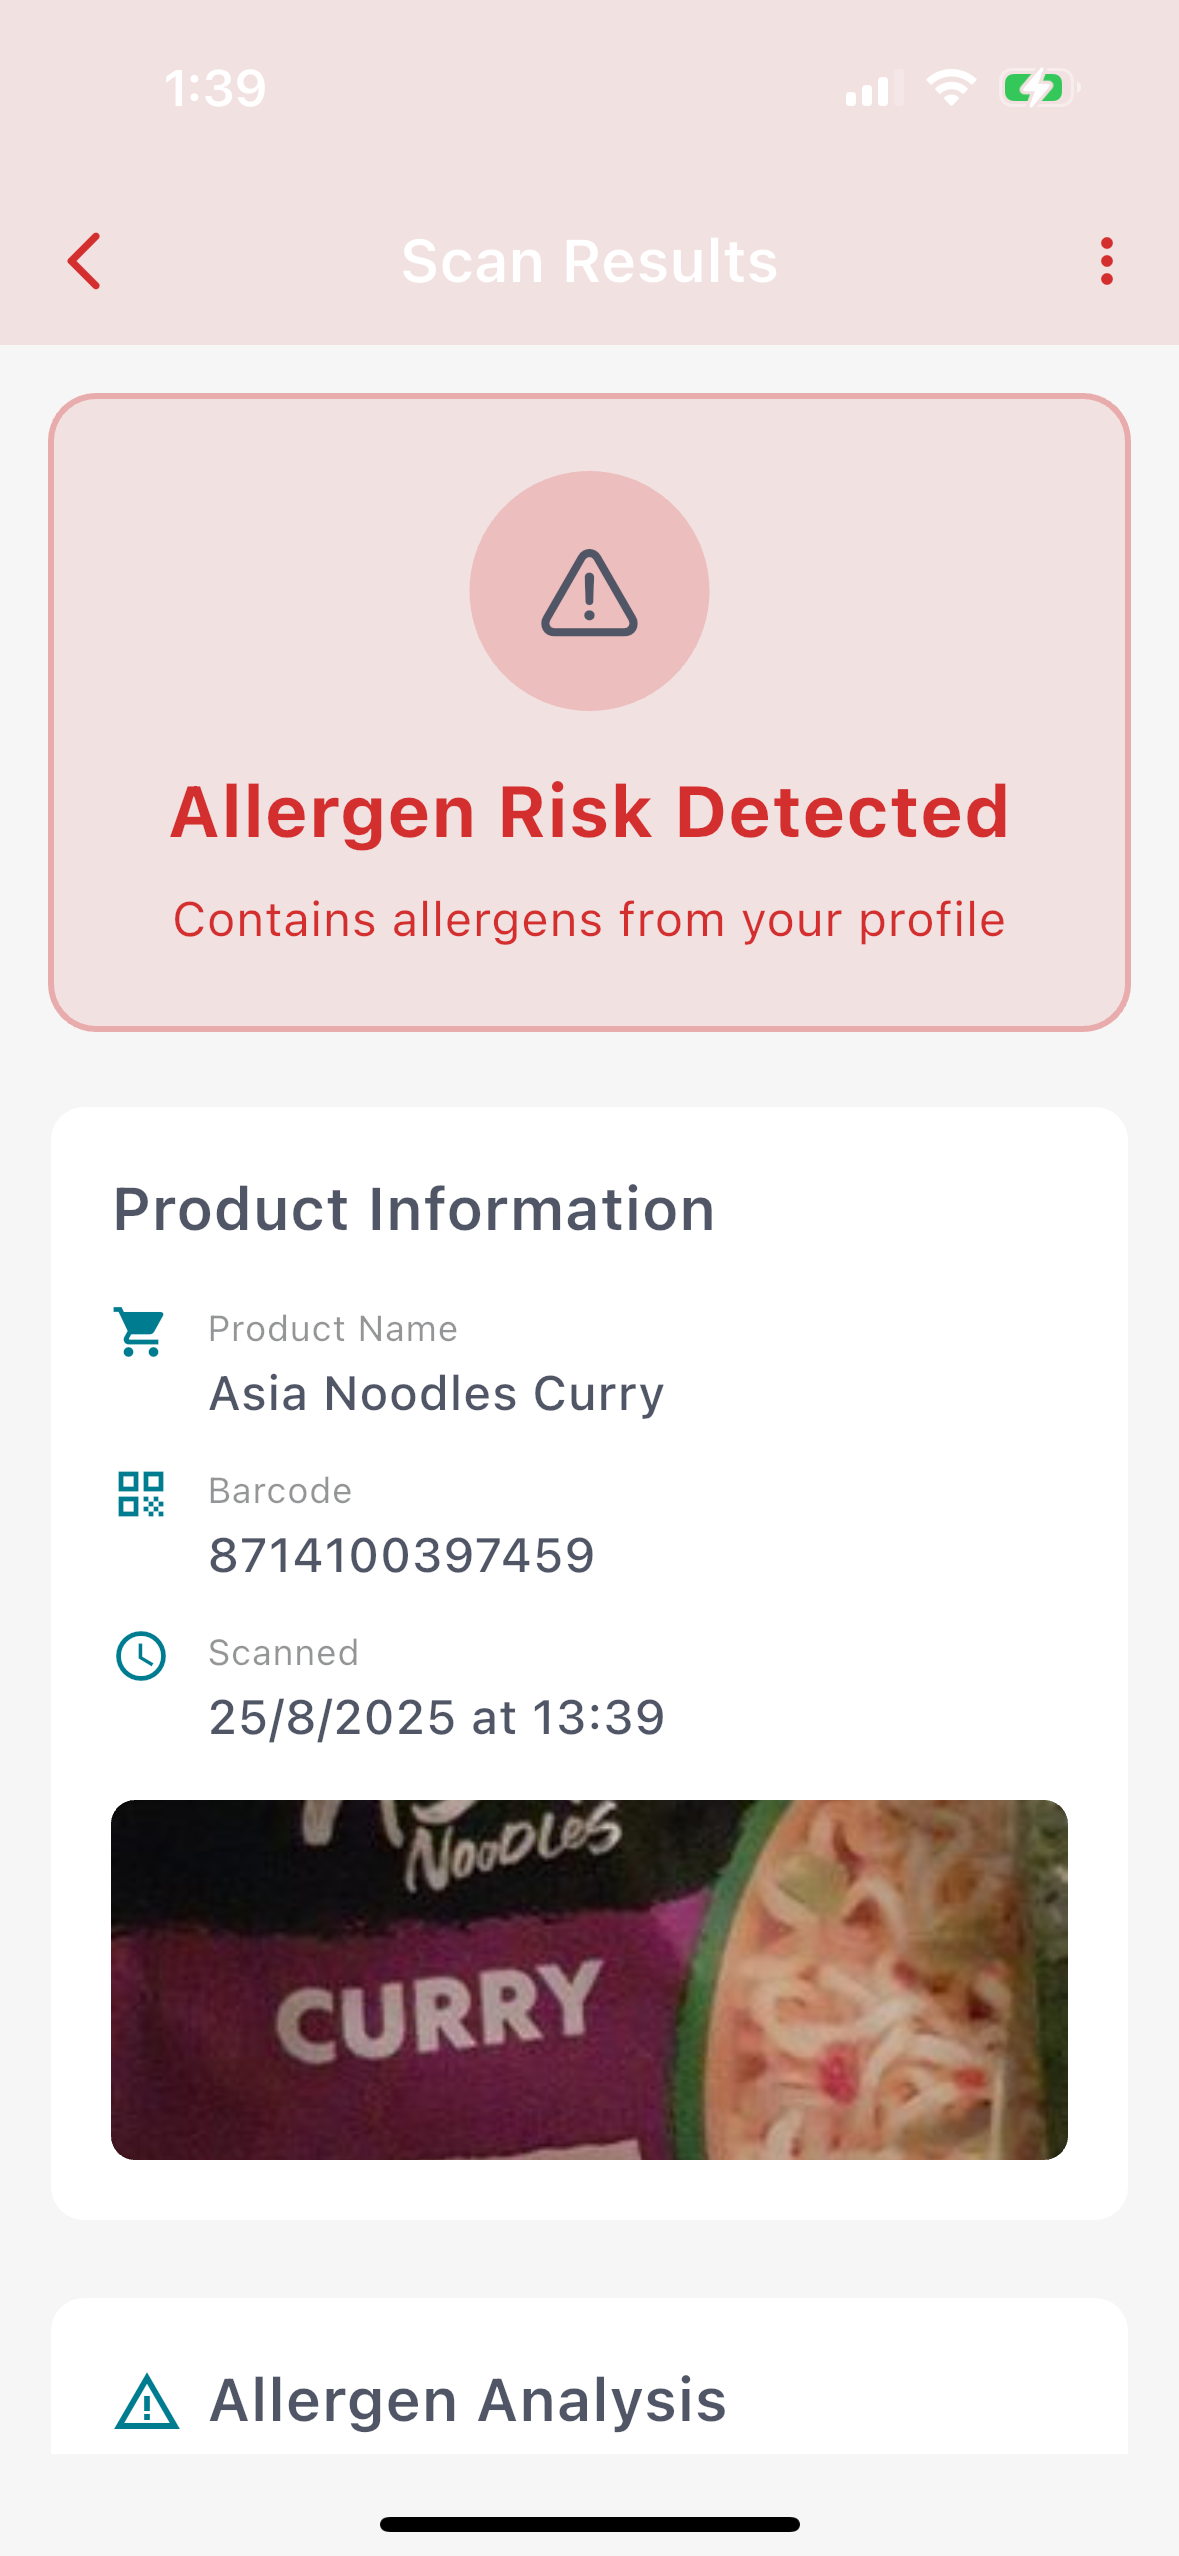
\includegraphics[width=0.9\textwidth,height=0.4\textheight,keepaspectratio]{Figures/barcode_scanner_result1.png}
    \end{minipage}
    \hfill
    \begin{minipage}[b]{0.3\textwidth}
        \centering
        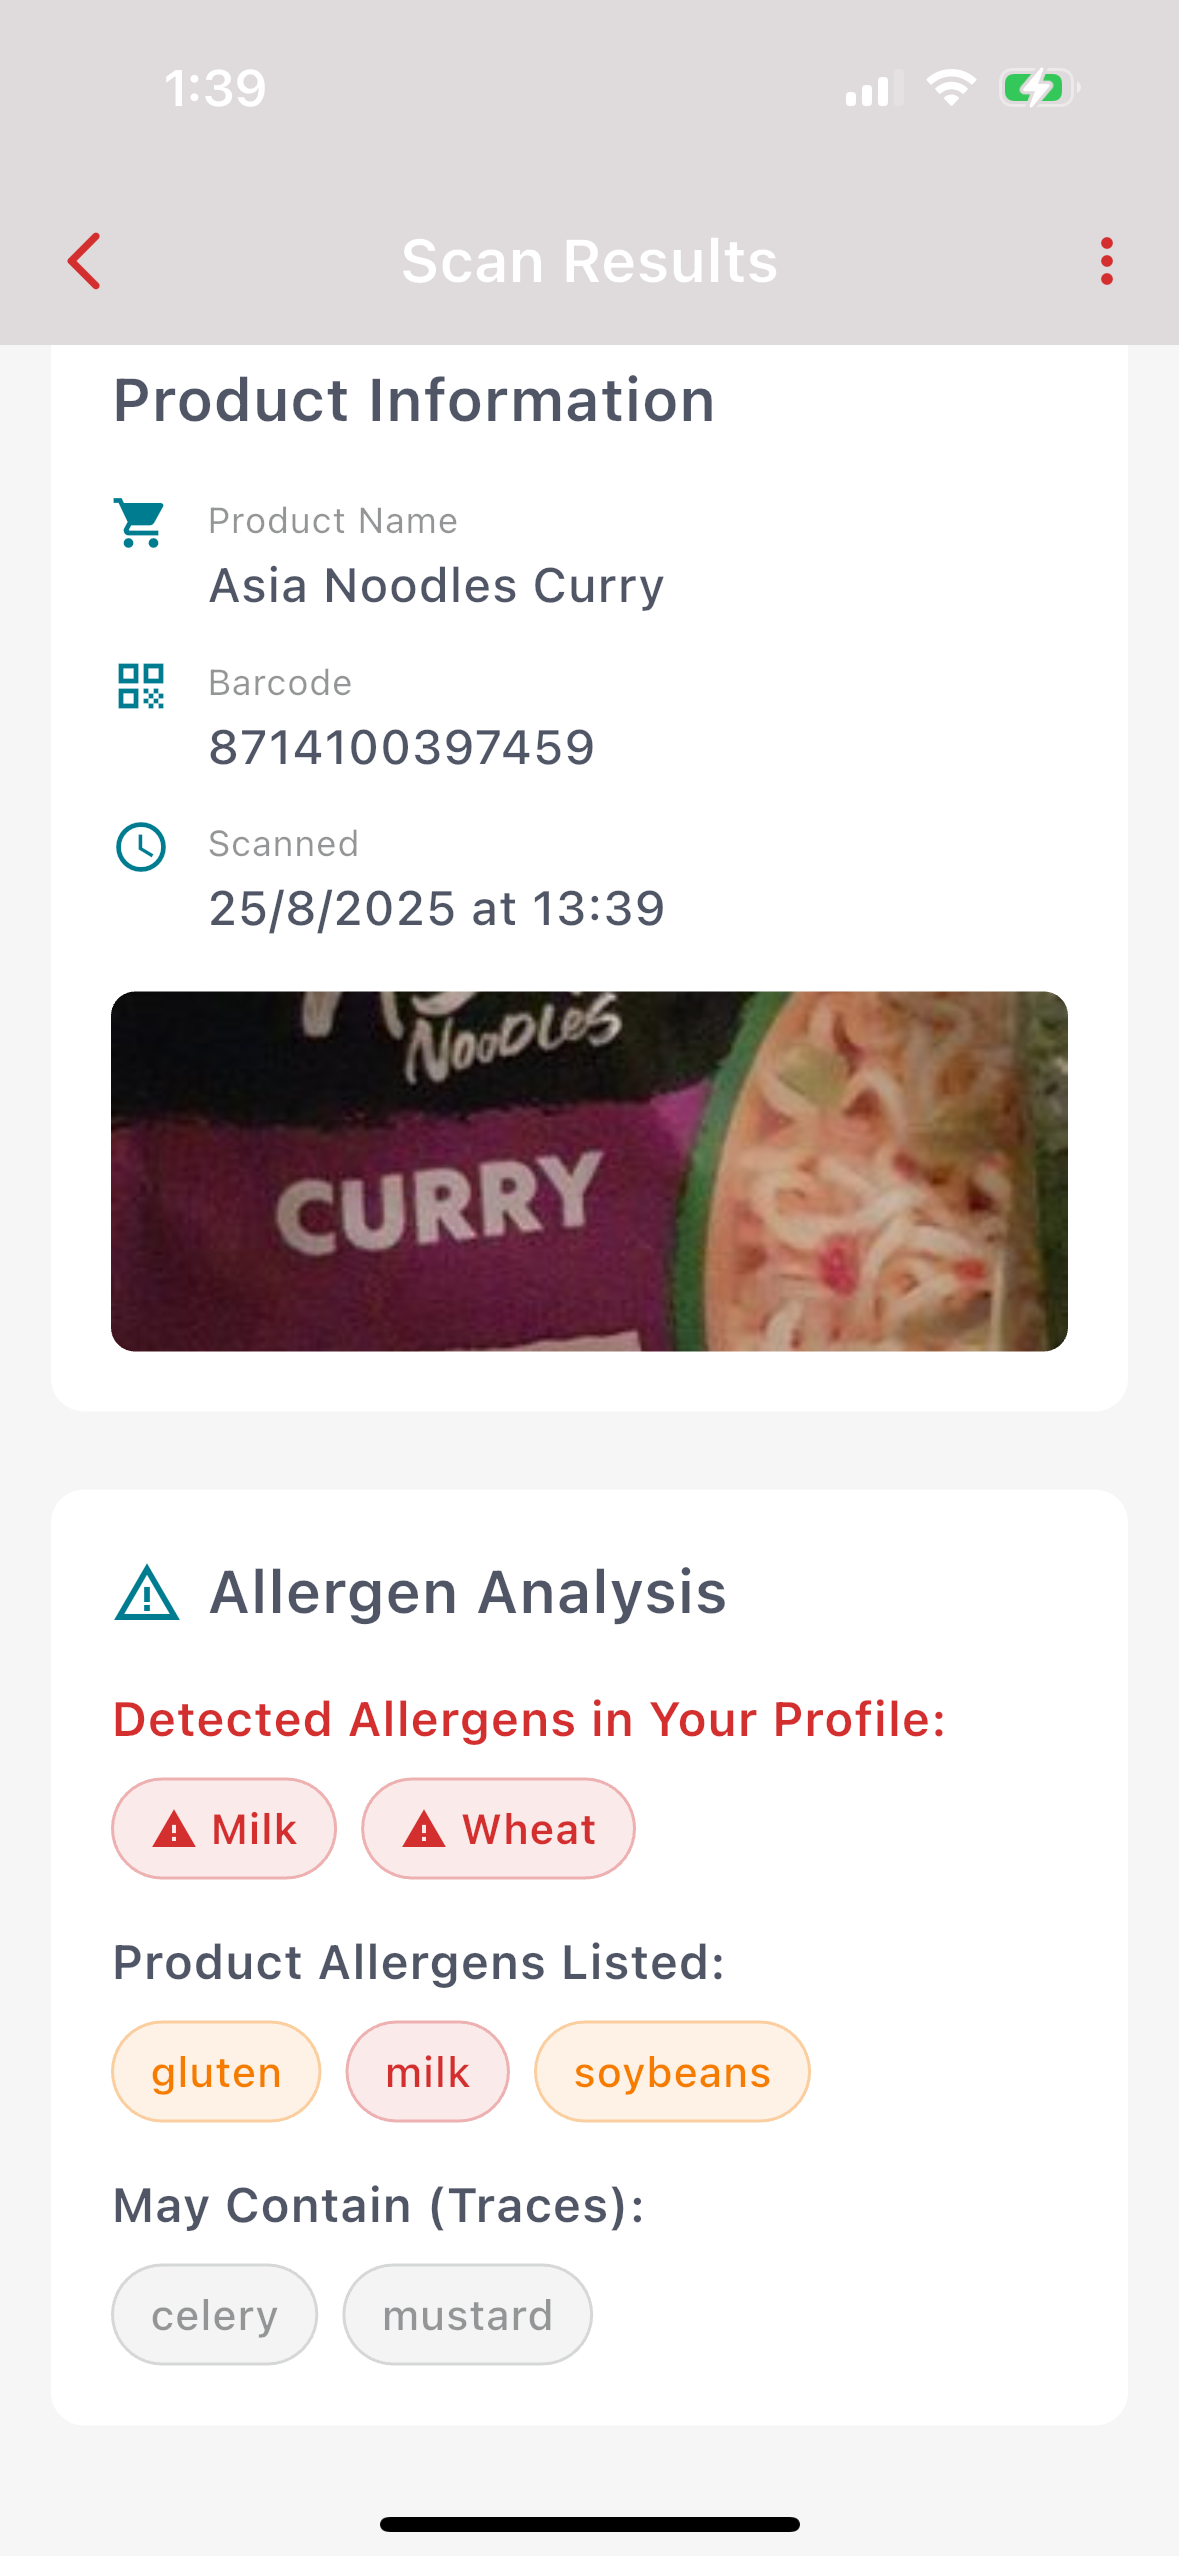
\includegraphics[width=0.9\textwidth,height=0.4\textheight,keepaspectratio]{Figures/barcode_scanner_result2.png}
    \end{minipage}
    \caption{Barcode Scanner Interface and Product Analysis Results}
    \label{fig:barcode-scanner-screenshots}
\end{figure}


\subsection{Camera-Based Barcode Detection and API Selection}

The scanning system utilizes the mobile scanner plugin for Flutter, providing standard barcode detection capabilities with support for common formats including UPC and EAN codes. The implementation includes basic camera controls with back-facing camera preference, no-duplicate detection speed settings, and manual entry fallback for cases where camera scanning fails.

For product data retrieval, two primary endpoints were considered for the Irish market: GS1 Ireland's commercial database service requiring paid subscriptions and licensing agreements, and OpenFoodFacts' free, open-source collaborative database. OpenFoodFacts was selected for the current implementation due to its accessibility, comprehensive coverage of international products, and alignment with the application's development timeline and budget constraints. The system queries the OpenFoodFacts API endpoint at `https://world.openfoodfacts.org/api/v0/product/[barcode].json` with appropriate user agent identification for responsible API usage.

The allergen detection process retrieves product information including product name, ingredient text, allergen tags, and trace tags from the OpenFoodFacts database. The system performs allergen matching by comparing user allergy profiles against product allergen tags, trace tags, and ingredient text using both exact matching and common allergen variations (such as matching "milk" with "dairy", "lactose", "casein", or "whey"). Results are categorized into simple verdicts of safe, risky, or unknown, with matched allergens highlighted for user awareness. All scan results are stored in Firebase Firestore for personal history tracking and future reference.






\clearpage

\chapter{Evaluation}
\label{chap:evaluation}

\section{Testing Methodology}
Evaluation of the \textit{AllerTeens} application was conducted through a combination of clinical expert review, academic oversight, and Patient and Public Involvement (PPI) sessions with adolescents. Ethical approval was secured in advance, ensuring compliance with GDPR standards and informed consent procedures for minors and their guardians.  

The evaluation procedure was broken down into two streams. The first one consisted of meetings with the Paediatric Allergy Unit of Cork University Hospital (CUH) and with the academic supervisors who assessed prototype to confirm its integration with allergy treatment protocols and its adherence to best allergy management practices. They assessed the precision of the emergency features, the educational content outlined, safety protocols regarding reminders and symptom logging, and overall, safety of the functions.

The second stream consisted of structured PPI evaluation with the same group of adolescents who had previously participated in the Patient and Public Involvement (PPI) sessions described in Chapter~\ref{chap:methodology}. These participants engaged directly with the prototype, completing a predefined set of tasks that reflected core use cases of the application. Tasks included account creation and profile setup, navigating AI training scenarios, using reminders, logging accidental exposures, scanning food products, and exploring the Learn module. Each task was rated on success, ease of use, usefulness, and enjoyment using a 1-5 scale.  

In preparation for the evaluation sessions, the application's stability was ensured through extensive unit and widget testing. Testing of the application's structure and logic, including form submission, module navigation, and data metering with Firebase, was done using the Flutter testing framework which validates interface components and logic. Integration tests were performed to validate the proper storage and retrieval of user data from Firestore, including the triggering of reminders and notifications.

In addition, specific attention was given to AI module testing. Calls to the OpenAI endpoint were validated for consistency and reliability, ensuring that speech-to-text transcription, text-to-speech synthesis, and scenario-based dialogue generation performed as intended. Edge cases, such as prolonged silence or ambiguous user responses, were tested to verify system stability. The accuracy of speech-to-text recognition was monitored under varying input conditions, and text-to-speech playback was tested across different devices to confirm quality and responsiveness.  

To supplement live demonstrations, a video recording was produced using QuickTime Player of the application running on the Xcode simulator (iPhone 16 Pro). This recording showcased the core features developed at that stage, including the exposure logging module, integrated calendar, reminder system, and AI training scenario. The video was presented in joint evaluation meetings with domain experts and the CUH clinical team, allowing stakeholders to observe the workflow without requiring each participant to operate the application directly.  

Feedback from this demonstration emphasised several key directions for refinement. Clinical experts recommended increasing the complexity of scenario-based training to better reflect real-world social and environmental challenges. They also suggested broadening the AI training to include progressively difficult levels, such as handling peer pressure or navigating noisy environments. The barcode scanner was highlighted as a particularly valuable addition to support safer food choices, reinforcing the importance of its integration in subsequent iterations.  

This method provided thorough evaluation by integrating automated unit testing, focused verification of AI endpoints, organized PPI sessions, as well as expert appraisal via live and recorded prototype evaluations. It confirmed the system's AI reliability, usability, and clinical relevance as well. The next parts describe the comments received from the adolescents and from the clinical specialists independently.



\section{Expert and Clinical Feedback}
Feedback from domain experts and the CUH clinical team reinforced the adolescents' positive reception, while also validating the application's clinical safety and relevance. Experts emphasised that the application addressed persistent gaps in adolescent allergy care, particularly the tendency to forget adrenaline pens and the difficulties of managing allergies in social environments.  

They highlighted that the design achieved an appropriate balance between safety and engagement. Offline emergency access was noted as essential, while the clarity and structure of educational materials were regarded as suitable for adolescent users. Experts also cautioned that gamification, while beneficial for motivation, should remain carefully moderated to ensure that life-saving protocols are not trivialised.  


\section{Feedback from Adolescents}
Adolescents consistently rated most tasks highly, and most features received scores of 4 to 5 for ease, usefulness, and enjoyment, based on the 1-5 evaluation scale described in Chapter~\ref{chap:methodology}. The AI training module emerged as the most engaging component, especially scenarios involving restaurants, dinners with friends, school trips, and parties(see Table~\ref{tab:ppi-feedback}). Participants reported that these contexts felt realistic and helped them practice allergy disclosure under pressure.  

Practical issues were noted in the training module, particularly with speech-to-text accuracy when microphones were held too far away. This led to the recommendation of introducing a help dialogue at the beginning of training sessions to guide correct microphone use. Advanced scenarios involving ingredient-based questioning were found to be confusing and were simplified for clarity.  


\begin{table}[htbp]
\centering
\small
\caption{Summary of adolescent feedback on prototype tasks (N=6)}
\label{tab:ppi-feedback}
\renewcommand{\arraystretch}{1.3}
\begin{tabularx}{\textwidth}{|c|X|c|c|c|X|}
\hline
\textbf{No.} & \textbf{Task} & \textbf{Ease} & \textbf{Usefulness} & \textbf{Enjoyment} & \textbf{Observed Issues / Suggestions} \\
\hline
1 & Sign up with email \& verify account & 5 & 5 & 5 & None \\
2 & Set up allergy profile (allergens, medical info, contact) & 5 & 5 & 5 & None \\
3 & Navigate to AI Beginner Scenario & 5 & 5 & 5 & Add guide dialogue for first-time users \\
4 & Complete Advanced Scenario & 4 & 5 & 5 & Remove ingredient-based questioning \\
5 & Group Scenario (party/dinner with friends) & 4 & 5 & 5 & Speech-to-text mishearing if mic held away \\
6 & Scan barcode from packaged food & 5 & 5 & 5 & None \\
7 & Log accidental exposure in tracker & 5 & 5 & 5 & None \\
8 & View Learn module and search allergen info & 5 & 5 & 5 & None \\
9 & Emergency contact button (without calling) & 5 & 5 & 5 & None \\
10 & Receive adrenaline pen reminder notification & 5 & 5 & 5 & Suggested event-specific reminders \\
\hline
\end{tabularx}
\end{table}


Reminders and logging functions received strong approval. Adolescents highlighted the value of the calendar-linked "Yes/No" pen carriage log for improving accountability, and suggested that reminders should also support scheduling for specific events such as school trips or parties. The barcode scanner was praised for its simplicity and speed, while the Learn module was considered helpful for quick reference to allergen information. In addition, some participants suggested incorporating playful elements such as mini-games or a translator for dining abroad, underlining the desire for both practicality and engagement.

At the end of the session, a short survey indicated that all participants rated their likelihood of continued use at the maximum score (5/5). They emphasised the novelty of the AI scenarios, the relevance of reminders, and the overall convenience of logging and scanning features as summarised in Table~\ref{tab:post-session-survey}.

\begin{table}[htbp]
\centering
\small
\caption{Post-Session Survey responses from adolescents (N=6)}
\label{tab:post-session-survey}
\renewcommand{\arraystretch}{1.2}
\setlength{\tabcolsep}{6pt}
\begin{tabular}{|c|p{6cm}|p{6cm}|}
\hline
\textbf{Q. No.} & \textbf{Survey Question} & \textbf{Summary of Responses} \\
\hline
1 & Which features did you like the most? Why? & AI training scenarios, group/friends simulation, restaurant ordering, reminders, barcode scanner, and logs were most frequently highlighted as enjoyable and realistic. \\
2 & Which features did you not like or found confusing? & None reported. \\
3 & Was anything missing from the app that you think would help you? & Suggestions included: ability to set event-specific reminders (e.g., before going to a party), and adding a language translator for use when dining abroad. \\
4 & How likely are you to keep using this app? (1-5) & All participants rated \textbf{5/5} (very likely). \\
5 & Any suggestions to make the app better? & Additional calendar-linked pen reminders and gamified/translator features. \\
\hline
\end{tabular}
\end{table}




\clearpage

\chapter{Conclusion}

This dissertation has described the design, development and evaluation of \textit{AllerTeens}, a mHealth application, which was created in partnership with the UCC School of Nursing and Midwifery and Paediatric Allergy Unit at Cork University Hospital (CUH). The system was developed to assist the adolescents with severe food allergies in their transition to the self-management process, which touches both the medical and psychosocial aspects.

The application integrates a range of features informed by literature, clinical expertise, and direct adolescent involvement through Patient and Public Involvement (PPI) sessions. Core contributions include:  
\begin{itemize}
    \item \textbf{AI-driven scenario training:} Waiter and group simulations that provide adolescents with realistic practice for allergy disclosure and decision-making in socially complex contexts such as restaurants, parties, and school trips.  
    \item \textbf{Real-time feedback and progress tracking:} Adaptive scoring and safety checks that reinforce correct behaviours while enabling users to track skill development over time.  
    \item \textbf{Symptom logging and reminders:} Calendar-integrated logs and adrenaline pen reminders that encourage accountability and adherence to safety practices.  
    \item \textbf{Educational and behavioural content:} Structured learning modules covering clinical, behavioural, and psychosocial guidance, ensuring adolescents have evidence-based resources for managing both the physical and emotional aspects of allergy care.  
    \item \textbf{Barcode scanning:} Integration with the OpenFoodFacts database to provide instant allergen checks on packaged foods, complementing real-world decision-making.  
\end{itemize}  

The analysis showed that the application is usable and clinically aligned. Teenagers reported features to be very useful and fun, with scenario training determined as the most interesting part. Relevance of reminders, logging of symptoms and emergency protocols was also confirmed by clinical experts, but it is also crucial to make gamification supportive and not trivializing life-saving practices.

\section{Reflection and Impact}
The study indicated the relevance of participatory design in digital interventions in health. Direct engagement with the adolescents meant that features were based on lived experiences, including forgetting how to use adrenaline pens or feeling anxious in a peer environment. Meanwhile, this clinical oversight based the system on best practice, without jeopardizing safety in any way. 

The project contributes not only to adolescent allergy care but also to broader telehealth research by demonstrating the value of immersive AI-driven training for self-management. Current literature highlights the underuse of gamification and interactive tools in allergy-focused applications \parencite{sullivan2024telehealth, gajardo2023gamification}, and this dissertation offers a working implementation that addresses these gaps.  

From a technical perspective, the project also verified the integration of Flutter, Firebase, OpenAI APIs, and other external databases into a unified cross-platform system, supporting offline access and future expansions. From a healthcare perspective, the project demonstrated the capacity of digital tools to enhance confidence, autonomy, and self-efficacy, three core elements of a successful adolescent transition to independence.


\section{Limitations}
While the \textit{AllerTeens} project has demonstrated strong feasibility and encouraging user engagement, several limitations must be acknowledged.  

First, the evaluation was conducted with a small cohort of six adolescents during the structured sessions described in Section~\ref{sec:ppi-sessions}. Although these Patient and Public Involvement (PPI) sessions provided valuable insights into usability and adolescent perspectives, they were short-term and did not extend over several months. As such, the evaluation could not capture longitudinal behaviours such as adherence, sustained engagement, or changes in anxiety and self-efficacy over time.  

Second, the AI training module currently consists of only a limited set of scenarios, namely waiter interactions and peer group contexts such as dinners with friends and birthday parties. While these reflect high-risk social situations highlighted by adolescents, the restricted variety limits generalisability to other everyday challenges (e.g., cross-contamination risks, travel, school trips or more complex food-service environments).  

Third, the barcode scanning functionality relies on the OpenFoodFacts database, which, while extensive, does not provide full coverage of all packaged food products available in Ireland. This may lead to situations where scans return no result, reducing reliability for users in real-world shopping or dining scenarios.  

In addition, the current version of the application emphasised breadth of feature integration rather than depth of clinical evaluation. Features such as reminders, symptom logs, and the Learn module were validated for usability and acceptability, but outcomes such as knowledge improvement, transition readiness, or reduction in food allergy anxiety were not formally measured.  

Finally, the system is dependent on cloud-based services for AI-driven training (speech-to-text, text-to-speech, and scenario dialogue). While offline functionality was implemented for reminders, logs, and emergency contact details, the reliance on internet connectivity may limit the app's utility in environments with poor network access.  

These limitations provide important direction for future work, particularly in extending evaluation to longitudinal clinical studies, expanding the range of AI-driven scenarios, strengthening database coverage, and improving offline capability.



\section{Future Work}
While the \textit{AllerTeens} MVP successfully demonstrated feasibility and impact, there are several opportunities for enhancement and expansion:  

\begin{itemize}
    \item \textbf{Expansion of Training Scenarios:} Future versions should include a broader range of AI-driven scenarios, incorporating more complex tasks such as handling cross-contamination queries, navigating noisy environments, and managing unexpected social pressures. Increasing scenario diversity will improve transferability to real-world contexts.  

    \item \textbf{Gamified Mini-Games:} Based on feedback from clinicians, parents, and adolescents, mini-games could be introduced to reinforce learning in a playful manner. Examples include symptom-medication matching, "safe vs unsafe food" selection, or reflex-based games like whack-a-mole where users identify correct responses under time pressure. Such activities can make repetitive training more engaging while strengthening knowledge retention.  

    \item \textbf{Enhanced Educational and Psychosocial Resources:} The educational and behavioural modules can be expanded with more in-depth clinical content drawn from CUH-validated resources. Psychosocial forms and questionnaires (e.g., for tracking anxiety, social stress, or confidence in disclosure) could be incorporated to provide richer data for both adolescents and clinicians. Literature suggests that monitoring psychosocial wellbeing is critical to supporting holistic self-management in chronic conditions \parencite{sullivan2024telehealth}.  

    \item \textbf{Quick Links to Allergen Information from Major Food Chains:}  
    During evaluation sessions, adolescents and clinicians highlighted the benefit of having direct access to allergen menus from popular food chains. Integrating quick links within the app would allow users to rapidly check allergen information before dining out, reducing uncertainty and supporting safer decision-making. This feature would complement the barcode scanner by extending allergen awareness to restaurant and takeaway contexts, which remain high-risk situations for adolescents \parencite{sullivan2024telehealth}.
 

    \item \textbf{Cross-Cultural and Multilingual Support:} Translation features for dining abroad were suggested during PPI sessions. Future iterations could implement multilingual training scenarios and allergen lookups to broaden accessibility and support adolescents in diverse cultural settings.  

    \item \textbf{Clinical Evaluation and Trial Design:}  
    A key future step will be conducting a minimal clinical evaluation followed by a structured trial to establish the app's effectiveness. This could involve a control group receiving usual care compared against an intervention group with access to \textit{AllerTeens} over a defined period (e.g., 6-12 months).  
    Evaluation metrics would include:
    \begin{itemize}
        \item \textit{Usage analytics:} frequency of feature use (e.g., training modules, reminders, logs).  
        \item \textit{Satisfaction measures:} adolescent-reported usability and acceptability.  
        \item \textit{Clinical outcomes:} knowledge improvement, transition readiness, reduction in food-allergy-related anxiety, and confidence in self-disclosure.  
    \end{itemize}
    This evaluation pathway would provide the necessary evidence base for clinical adoption and integration into adolescent allergy care.
\end{itemize}  


Altogether, the dissertation has shown that an adolescent-oriented digital health application has the potential to integrate artificial intelligence, gamification, and clinical evidence to develop a secure, interactive, and scalable support system in allergy self-management. By grounding design in both adolescent experiences and clinical oversight, \textit{AllerTeens} achieves a balance between usability and safety.  

The results validate the possible role of mHealth solutions to improve adolescent autonomy in the management of chronic conditions and provide a guiding path to the successive development and clinical integration. Although the project is just a stepping stone, its principles are solid and its future upgrades are promising to change the way food allergic young people live their lives.


\appendix
\chapter{Supporting Sources for Learn Module}
\label{app:resources}

This appendix provides the supplementary resources that informed the educational and psychosocial content included in the \textit{Learn} module of AllerTeens. These include youth-focused guides, clinical booklets, websites, and peer-reviewed references. They were reviewed in collaboration with CUH clinicians to ensure adolescent relevance and medical accuracy.

\section*{Websites and Booklets}
\begin{itemize}
    \item \href{https://spunout.ie/}{Spunout website - Youth-Driven Support and Information}
    \item \href{https://steppingup.ie/}{SteppingUp.ie - Transitioning to Adult Healthcare in Ireland}
    \item \href{https://www.hse.ie/eng/about/who/cspd/transition-of-care/toc-framework.pdf}{Transition of Care from Paediatric to Adult Services: A National Framework (HSE)}
    \item \href{https://media.gosh.nhs.uk/documents/Booklet.PDF}{Great Ormond Street Hospital - Transitioning to adult services workbook}
    \item \href{https://cphealthcaretransition.eu/wp-content/uploads/2024/08/Information-booklet-for-young-people-1.pdf}{Information for Young People with Cerebral Palsy - Healthcare transitions (2024)}
    \item \href{https://www2.hse.ie/services/moving-from-child-to-adult-health-services/}{Moving from child to adult health services (HSE)}
    \item \href{https://www.epilepsy.ie/sites/www.epilepsy.ie/files/Teens_Booklet\%202018.pdf}{Epilepsy Ireland - Moving forward: a guide for young people with epilepsy (2018)}
    \item \href{https://www.epilepsy.ie/sites/www.epilepsy.ie/files/How2tell_BOOKLET.pdf}{Trinity College Dublin - How 2 Tell booklet (2017)}
    \item \href{https://foodallergycanada.ca/wp-content/uploads/NDHB_eng_web.pdf}{Living Confidently with Food Allergy: A Guide for Parents and Families (2015)}
    \item Teenage Allergy Handbook, Dr.~Linda McDonald \& Lorraine Bell (2018), Paediatric Allergy Service, Southern Trust, Northern Ireland
    \item \href{https://foodallergycanada.ca/wp-content/uploads/6_StressAndAnxiety-Web.pdf}{Stress \& Anxiety Related to Food Allergy (Food Allergy Canada)}
    \item \href{https://www.anaphylaxis.org.uk/about-us/}{Anaphylaxis UK - About Us}
    \item \href{https://www.foodallergycounselor.com/}{The Food Allergy Counsellor - Resources on anxiety, mindset, and parenting}
\end{itemize}

\section*{Peer-Reviewed and Clinical Sources}
\begin{itemize}
    \item Baseggio Conrado A, Ierodiakonou D, Gowland MH, Boyle RJ, Turner PJ. \textit{Food anaphylaxis in the United Kingdom: Analysis of national data, 1998-2018}. BMJ. 2021;372. doi:10.1136/bmj.n251
    \item Umasunthar T, Leonardi-Bee J, Hodes M, et al. \textit{Incidence of fatal food anaphylaxis in people with food allergy: a systematic review and meta-analysis}. Clin Exp Allergy. 2013;43(12):1333-1341. doi:10.1111/cea.12211
    \item Smith H, Brown C, Robertson A, Stuttaford L, Rashid R, Jones CJ. \textit{The Experience of Being Tested for Allergies; the Views of Children and their Parents}. J Allergy Ther. 2019;10(1). doi:10.4172/2155-6121.1000287
    \item Aronson J. \textit{"Where name and image meet" - the argument for "adrenaline"}. BMJ. 2000;320:506-509. doi:10.1136/bmj.320.7233.506
    \item Agostino H, Toulany A. \textit{Considerations for privacy and confidentiality in adolescent health care service delivery}. Paediatr Child Health. 2023;28(3):172-177. doi:10.1093/pch/pxac117
    \item Chang F, Eng L, Chang C. \textit{Food Allergy Labeling Laws: International Guidelines for Residents and Travelers}. Clin Rev Allergy Immunol. 2023;65(2):148-165. doi:10.1007/s12016-023-08960-6
    \item Heraghty F, Flynn N, Hurley S, et al. \textit{WOTNUT: Nut Allergic Children and Their Parents Are No Better at Identifying Nuts Than Controls Without Nut Allergy}. J Allergy Clin Immunol. 2023;151(2):AB172. doi:10.1016/j.jaci.2022.12.538
    \item Dominguez S, Théolier J, Lizée K, et al. \textit{"Vegan" and "plant-based" claims: risk implications for milk- and egg-allergic consumers in Canada}. Allergy Asthma Clin Immunol. 2023;19(1). doi:10.1186/s13223-023-00836-w
    \item Vassilopoulou E, Karathanos A, Siragakis G, et al. \textit{Risk of allergic reactions to wine in milk, egg, and fish-allergic patients}. Clin Transl Allergy. 2011;1(1):1-4. doi:10.1186/2045-7022-1-10
    \item European Food Safety Authority. \textit{Opinion of the Panel on dietetic products, nutrition and allergies related to a notification from CEPS on nuts used in distillates for spirits}. EFSA Journal. 2007;5(6). doi:10.2903/j.efsa.2007.482
    \item Baig M. \textit{Shellfish allergy and relation to iodinated contrast media: United Kingdom survey}. World J Cardiol. 2014;6(3):107. doi:10.4330/wjc.v6.i3.107
    \item Maloney JM, Chapman MD, Sicherer SH. \textit{Peanut allergen exposure through saliva: Assessment and interventions to reduce exposure}. J Allergy Clin Immunol. 2006;118(3):719-724. doi:10.1016/j.jaci.2006.05.017
    \item Turner P, Dowdall N. \textit{Flying with nut and other food allergies: unravelling fact from fiction}. Arch Dis Child. 2024. doi:10.1136/archdischild-2024-327848
    % \item Feleszko W, Ryczaj K, Chojnowska-Wójtowicz M, et al. \textit{Prevalence of major food allergens in skincare products for atopic dermatitis}. Adv Dermatol Allergol. 2023;XL(6):762-765. doi:10.5114/ada.2023.13381
    \item Ruran HB, D'Ambrosi G, Dupuis R, et al. \textit{Household Food Allergen Exclusion Practices and Food Allergy-Related Psychosocial Functioning}. JAMA Netw Open. 2024;7(12):e2452646. doi:10.1001/jamanetworkopen.2024.52646
    \item Sheehan M, Lins de Holanda Coelho G, Kelleher M, Hourihane JOB, Byrne A, Dunn Galvin A. \textit{The impact of an evidence-based myth-busting intervention on maternal food allergy-related quality of life, anxiety and self-efficacy}. Clin Exp Allergy. 2024. doi:10.1111/cea.14494
\end{itemize}

\section*{Additional Clinical and Information Sources}
\begin{itemize}
    \item Citizens Information - Prescribed drugs and medicines (HSE Schemes and Allowances)  
    \item Cleveland Clinic - Atopy: Disease, Causes, Triggers, Conditions \& Treatment  
    \item Food Safety Authority of Ireland - Wine and Allergens  
    \item \href{https://erudus.com/editorial/the-food-agenda/how-allergens-hide-in-alcohol}{Erudus - How Allergens Hide in Alcohol (2022)}  
    \item Food Safety Authority of Ireland (2015) - Allergen Information for Non-Prepacked Food  
    \item Epipen - Patient Information  
    \item Jext - Patient Information  
    \item Anapen - Patients \& Carers Resource Centre  
    \item HSE, National Immunisation Office - Supporting Information for Vaccinations in General Practice (2024)  
    \item Allergy 250K for Teens and Young Adults - Resource hub for young Australians with severe allergy  
\end{itemize}


\printbibliography
\end{document}

